\documentclass[12pt,letterpaper]{article}

%% ---- Paquetes esenciales ----
\usepackage[utf8]{inputenc}
\usepackage[T1]{fontenc}
%\usepackage[es-noshorthands]{babel}
\usepackage{geometry}
\usepackage{amsmath,amssymb}
\usepackage{graphicx}
\usepackage{booktabs}
\usepackage{array}
\usepackage{hyperref}
\usepackage{setspace}
\usepackage{parskip}
\usepackage{titlesec}
\usepackage{fancyhdr}
\usepackage{cite}
\usepackage{float}
\usepackage{longtable}
\usepackage{caption}

\geometry{letterpaper, top=2.5cm, bottom=2.5cm, left=3cm, right=2.5cm}

\onehalfspacing

\hypersetup{colorlinks=true, linkcolor=black, citecolor=black, urlcolor=black, hidelinks}

\titleformat{\section}{\large\bfseries}{}{0em}{}[\titlerule]
\titleformat{\subsection}{\normalsize\bfseries}{}{0em}{}

\pagestyle{fancy}
\fancyhf{}
\rhead{\small Proyecto de Grado}
\lhead{\small Universidad Distrital Francisco Jos\'e de Caldas}
\cfoot{\thepage}

\graphicspath{{img/}}

\begin{document}

%% ---- Portada ----
\begin{titlepage}
\begin{center}
{\large \textbf{UNIVERSIDAD DISTRITAL FRANCISCO JOS\'E DE CALDAS}}\\[0.3cm]
{\large Facultad de Ingenier\'ia}\\[0.3cm]
{\large Proyecto Curricular de Ingenier\'ia de Sistemas}\\[2cm]
{\LARGE \textbf{Control y Observaci\'on Basados en el Operador de Koopman para un Sistema Hidr\'aulico No Lineal de Tanques Acoplados: Validaci\'on Experimental y Comparaci\'on con M\'etodos de Referencia}}\\[2cm]
{\large \textbf{Trabajo de Grado}}\\[0.5cm]
{\large Modalidad: Investigaci\'on}\\[2cm]
\begin{tabular}{ll}
\textbf{Estudiante:} & Wilder Steven Hern\'andez Manosalva \\
\textbf{C\'odigo:}   & 20212020135 \\
\textbf{Correo:}     & wshernandezm@udistrital.edu.co \\[0.5cm]
\textbf{Docente director:} & Duv\'an Andr\'es T\'ellez Castro \\
\textbf{Correo:}     & duatellezc@udistrital.edu.co \\
\end{tabular}\\[3cm]
{\large Bogot\'a D.C., 2026}
\end{center}
\end{titlepage}

\tableofcontents
\newpage

%% ================================================================
\section{Formulación del Problema}
\label{sec:problema}

En múltiples industrias, como el procesamiento de fluidos, el tratamiento de agua,
las plantas químicas y los sistemas de generación térmica, los procesos hidráulicos
conformados por tanques acoplados constituyen una clase de sistemas dinámicos no lineales cuyo
comportamiento está gobernado por fenómenos como flujos de descarga no lineales,
restricciones en los actuadores y variaciones paramétricas. En estos procesos, el
control preciso de los niveles y la estimación confiable de los estados no medibles
son requisitos indispensables para garantizar la seguridad operativa, la eficiencia
energética y el cumplimiento de las especificaciones de calidad.

El diseño simultáneo de controladores y observadores para sistemas no lineales
plantea, sin embargo, desafíos considerables. Los enfoques clásicos basados en
linealización, como el control predictivo lineal (MPC) y los observadores tipo
Luenberger, degradan su desempeño cuando el sistema se aleja del punto de operación
nominal. La validez de una única linealización está restringida a un entorno
reducido del punto de equilibrio. Las alternativas no lineales, como el Control
Predictivo No Lineal (NMPC) y el Estimador por Horizonte Deslizante (MHE), ofrecen
mayor precisión al operar directamente sobre el modelo no lineal, pero demandan una
capacidad computacional elevada y dependen críticamente de modelos no lineales
exactos, cuya identificación resulta costosa y sensible a incertidumbres.

Los métodos puramente basados en datos, como redes neuronales o modelos de caja
negra, logran capturar no linealidades complejas. Sin embargo, sacrifican
interpretabilidad, dificultan las garantías formales de estabilidad y presentan
limitaciones para su integración en esquemas de control óptimo. Persiste, en
consecuencia, una brecha metodológica entre las técnicas lineales (tratables
computacionalmente pero imprecisas frente a no linealidades) y las no lineales (más
exactas pero costosas y de difícil implementación).

El operador de Koopman ha emergido como una alternativa que permite representar
sistemas no lineales mediante dinámicas lineales en un espacio de observables de
dimensión extendida, preservando la estructura matemática, la interpretabilidad y la
compatibilidad con las herramientas clásicas de control y estimación. A pesar de los
avances teóricos recientes, la aplicación integrada de un observador y un
controlador basados en Koopman sobre sistemas hidráulicos reales ha sido escasamente
documentada. En particular, no se ha caracterizado de manera rigurosa el desempeño
de un esquema Koopman completo, que integra observador y controlador, frente a
métodos de referencia como el par NMPC--MHE, en condiciones de ruido de medición,
medición parcial del estado y cambios escalonados de referencia sobre una planta
física real.

Esta ausencia de validación experimental conjunta constituye el problema central que
aborda este trabajo: no se conoce, con evidencia experimental, si las ventajas
teóricas del enfoque Koopman, reportadas hasta ahora principalmente en simulación,
se mantienen cuando el observador y el controlador operan juntos en lazo cerrado
sobre hardware real, sujeto a dinámicas no modeladas, ruido de sensores e
incertidumbre paramétrica.

\subsection{Pregunta de Investigación}

¿En qué medida un esquema completo de control predictivo y observación de estados
basado en el operador de Koopman, identificado mediante EDMD (Extended Dynamic Mode
Decomposition) y complementado con un estado integrador en el lazo de control,
puede igualar o superar el desempeño del par NMPC--MHE en una planta física de tres
tanques acoplados, en términos de seguimiento de referencia, estimación de estados
no medibles y eficiencia computacional, bajo condiciones de ruido de medición,
medición parcial del estado y cambios escalonados de referencia?

%% ================================================================
\section{Introducción}
\label{sec:introduccion}

El control y la estimación de estados en sistemas hidráulicos no lineales
constituyen un desafío central en la ingeniería de procesos. La dinámica de los
tanques acoplados, gobernada por la ley de Torricelli y por acoplamientos que
transitan entre regímenes laminares y turbulentos, exhibe un comportamiento
fuertemente no lineal que limita la aplicabilidad de las técnicas lineales clásicas
fuera de un entorno reducido del punto de operación. Los métodos avanzados como el
NMPC y el MHE ofrecen alta precisión en todo el rango de operación, pero a costa de una elevada
demanda computacional, lo que dificulta su implementación en plataformas embebidas
con recursos limitados.

En este contexto, el operador de Koopman emerge como un marco matemático que permite
representar sistemas no lineales mediante modelos lineales en un espacio de
observables de dimensión extendida \cite{koopman1931, williams2015}. Esta
linealización global, basada exclusivamente en datos, habilita el uso de
herramientas de control y estimación lineales, como el MPC cuadrático y el
observador de Luenberger, preservando al mismo tiempo la fidelidad de la dinámica no
lineal subyacente en todo el rango de operación cubierto por los datos de
entrenamiento. Trabajos previos han demostrado en simulación que el controlador
KoopmanMPC iguala al NMPC en precisión de seguimiento con una reducción sustancial
del costo computacional \cite{korda2018, tellez2022}, y que el observador de
Luenberger formulado en el espacio de Koopman puede alcanzar una precisión
comparable a la de estimadores no lineales en lazo abierto \cite{surana2016,
netto2020}.

No obstante, la validación experimental del esquema completo en lazo cerrado, que
integra el observador de Luenberger con el KoopmanMPC, no había sido realizada para
el sistema no lineal de tres tanques. Tampoco se había abordado su comparación
cuantitativa rigurosa frente al benchmark MHE+NMPC en una planta física real antes
de esta investigación. Los escasos trabajos que integran ambos componentes lo hacen
exclusivamente en simulación, dejando abierta la pregunta de si las ventajas
teóricas del enfoque Koopman se trasladan efectivamente al entorno experimental,
donde están presentes ruido de sensores, dinámicas no modeladas, restricciones de
actuadores e incertidumbre paramétrica.

El presente trabajo aborda esta brecha mediante el diseño, la construcción y la
validación experimental de un esquema completo de control predictivo y observación
de estados basado en el operador de Koopman para un sistema hidráulico de tres
tanques acoplados. La investigación comprende: (i) la construcción de una planta
física de laboratorio con componentes comerciales de bajo costo, incluyendo su
arquitectura electrónica de control; (ii) la calibración experimental de los
parámetros físicos del modelo no lineal; (iii) la identificación del modelo EDMD a
partir de datos generados sobre el modelo calibrado; y (iv) la ejecución de múltiples
corridas experimentales en lazo cerrado bajo una secuencia de referencias escalonadas
($0.10 \rightarrow 0.20 \rightarrow 0.15$ m), con ruido de medición y medición
parcial del estado, dado que solo los tanques 1 y 3 son sensados mientras que el
nivel del tanque 2 debe ser estimado.

El proceso de desarrollo de esta investigación fue iterativo, como se detalla en la
Sección~\ref{sec:discusion}. Las primeras corridas experimentales revelaron una
limitación estructural del observador de Luenberger en el espacio de Koopman, lo que
motivó la incorporación de un estado integrador con mecanismo de \textit{deadband}
que preserva íntegramente la arquitectura Koopman. El esquema resultante, denominado
Koopman, mantiene los mismos parámetros de sintonía del controlador que el NMPC de
referencia ($N=20$, $q=500$, $R_1$, $R_2$), garantizando una comparación justa entre
ambos esquemas.

Las contribuciones de este trabajo son, por tanto, cuatro. En primer lugar, se
presenta la construcción documentada de una planta física de tres tanques acoplados
con instrumentación de bajo costo (ESP32, sensores ultrasónicos HC-SR04, bombas de
diafragma R385), incluyendo su calibración experimental y arquitectura de control.
En segundo lugar, se presenta la primera validación experimental de un esquema
Koopman completo (observador más controlador) en lazo cerrado para un sistema
hidráulico no lineal con medición parcial, con comparación cuantitativa frente al
benchmark MHE+NMPC sobre dicha planta física, mediante diez corridas experimentales
independientes (cinco por esquema). En tercer lugar, se identifica y
caracteriza experimentalmente una limitación estructural del observador de
Luenberger en el espacio de Koopman: la acumulación de error de modelo por ausencia
de memoria temporal, agravada por la observabilidad débil del estado no medido a
$T_s=2$ s. Esta limitación explica la degradación observada en lazo cerrado frente
al benchmark.
En cuarto lugar, se propone y valida experimentalmente una estrategia de mitigación
basada en un integrador con \textit{deadband} en el espacio de Koopman, que elimina
el bias sistemático sin alterar la naturaleza convexa del problema de control,
permitiendo que el esquema Koopman mejorado supere al benchmark MHE+NMPC en
precisión de seguimiento en estado estacionario, manteniendo la ventaja
computacional del controlador cuadrático.

Esta investigación se apoya en dos contribuciones previas de los mismos autores, que
constituyen su base metodológica: un primer trabajo, aceptado en la conferencia
CoDIT 2026, validó en simulación el controlador KoopmanMPC con un diccionario
compacto de observables inspirado en la ley de Torricelli \cite{hernandez2026}; un
segundo trabajo, en revisión en la revista \textit{Sensors} (MDPI), extendió esta
validación al dominio experimental sobre la misma planta física, comparando el
observador de Luenberger en el espacio de Koopman con un Filtro Extendido de Kalman
\cite{hernandez2025sensors}. La presente tesis unifica y completa ambos trabajos al
integrar el observador y el controlador en un único lazo cerrado, comparándolo con
el benchmark MHE+NMPC y desarrollando la estrategia del integrador con
\textit{deadband} que no había sido explorada en las publicaciones previas.

El resto del documento se organiza de la siguiente manera: la
Sección~\ref{sec:marco} presenta el marco de referencia, incluyendo el modelo del
sistema, su linealización, el operador de Koopman y los métodos de estimación y
control empleados. La Sección~\ref{sec:metodologia} describe la metodología,
abarcando la construcción y calibración de la planta física, su arquitectura
electrónica, el entrenamiento del modelo EDMD y el diseño del observador y del
controlador. La Sección~\ref{sec:resultados} expone los resultados de simulación y
experimentales, incluyendo la comparación entre el esquema Koopman y el benchmark
MHE+NMPC. La Sección~\ref{sec:discusion} analiza e interpreta los hallazgos, con
énfasis en la limitación estructural identificada y en el impacto del integrador.
Finalmente, la Sección~\ref{sec:conclusiones} resume las conclusiones principales y
esboza líneas de trabajo futuro.

%% ================================================================
\section{Objetivos}
\label{sec:objetivos}

\subsection{Objetivo General}
\label{sec:objetivo_general}

Desarrollar un esquema de control predictivo y
observación de estados basado en el operador de Koopman, integrado por un
observador de Luenberger y un controlador KoopmanMPC con estado integrador, para
un sistema hidráulico no lineal de tres tanques acoplados con medición parcial,
en comparación cuantitativa con el benchmark MHE+NMPC sobre una planta física de
laboratorio.

\subsection{Objetivos Específicos}
\label{sec:objetivos_especificos}

\begin{enumerate}
    \item Revisar el estado del arte en teoría del operador de Koopman, el método
    EDMD y los métodos de control y estimación basados en datos para sistemas
    hidráulicos no lineales con medición parcial.

    \item Construir una planta física de tres tanques acoplados con componentes
    comerciales de bajo costo, instrumentada con un microcontrolador ESP32,
    sensores ultrasónicos HC-SR04 y bombas de diafragma R385, calibrando los
    parámetros físicos del sistema experimentalmente.

    \item Identificar el modelo del sistema de tres tanques en las coordenadas del
    operador de Koopman mediante la técnica EDMD, empleando un diccionario de ocho
    observables con interpretación física.

    \item Diseñar el observador de Luenberger en el espacio de Koopman, mediante
    el barrido sistemático de la ganancia $L$ obtenida por la ecuación algebraica
    de Riccati discreta (DARE), y el controlador predictivo KoopmanMPC con
    restricciones, bajo los mismos parámetros de sintonía que sus contrapartes de
    referencia (MHE y NMPC).

    \item Validar experimentalmente el esquema completo Koopman en lazo cerrado
    sobre la planta física, mediante su comparación cuantitativa con el benchmark
    MHE+NMPC en términos de precisión de seguimiento, bias en estado estacionario y
    tiempos de cómputo.
\end{enumerate}

%% ================================================================
\section{Justificación}
\label{sec:justificacion}

La estimación de estados en sistemas hidráulicos con medición parcial es una
necesidad transversal a múltiples sectores industriales, como el tratamiento de
agua, el procesamiento químico, la generación térmica y las redes de distribución
de fluidos, donde la instrumentación completa resulta inviable por razones de costo, acceso
físico o condiciones ambientales adversas. En estos escenarios, la capacidad de
inferir variables no medidas a partir de un conjunto reducido de sensores es tan
crítica como la propia acción de control, y el diseño de observadores precisos y
robustos para sistemas no lineales con restricciones constituye un problema abierto
de alta relevancia práctica.

Desde la perspectiva teórica, el operador de Koopman ofrece un marco matemático
riguroso que reconcilia la precisión de los modelos no lineales con la tratabilidad
de las herramientas lineales. A diferencia de los enfoques puramente empíricos, la
representación de Koopman preserva una estructura que habilita el análisis de
estabilidad y las garantías de convergencia, y ha demostrado ser eficaz para el
diseño de observadores lineales en el espacio elevado \cite{surana2016, netto2020}
y para la formulación de problemas de control predictivo con costo computacional
reducido \cite{korda2018, tellez2022}. Sin embargo, la mayoría de los trabajos que
integran simultáneamente un observador y un controlador basados en Koopman han
limitado su validación al ámbito de la simulación. Persiste, por tanto, una brecha
metodológica significativa: la ausencia de evidencia experimental sobre el
desempeño del esquema Koopman completo, que integra observador y controlador, en
lazo cerrado, y su comparación cuantitativa con el benchmark de referencia
constituido por el par MHE+NMPC.

Esta brecha resulta particularmente relevante en el contexto de los sistemas
hidráulicos acoplados, donde las no linealidades de Torricelli, las transiciones
laminares-turbulentas en los flujos de acoplamiento y las restricciones físicas de
los actuadores imponen condiciones que ningún modelo matemático puede capturar con
exactitud absoluta. En una planta real, la presencia de ruido de sensores,
dinámicas no modeladas, incertidumbre paramétrica y limitaciones en la tasa de
muestreo introduce discrepancias inevitables entre el modelo de predicción y el
comportamiento observado. Estas discrepancias afectan de manera diferenciada al
observador de Luenberger, un estimador recursivo de un solo paso, y al MHE, un
estimador basado en optimización sobre una ventana temporal. El impacto relativo de
estas diferencias sobre el desempeño global del lazo cerrado no había sido
caracterizado experimentalmente antes de este trabajo.

Desde el punto de vista práctico, el sistema de tres tanques acoplados es
ampliamente reconocido como banco de pruebas para técnicas de control no lineal
\cite{johansson2000}. Su combinación de no linealidades suaves, como los flujos de
Torricelli y los acoplamientos dependientes de la raíz cuadrada de la diferencia de
niveles, con restricciones físicas bien definidas lo hace adecuado para evaluar la
metodología propuesta en condiciones representativas de procesos industriales. El
hecho de que solo dos de los tres niveles sean medibles reproduce exactamente el
escenario de estimación parcial común en la industria. La construcción de la planta
con componentes comerciales de bajo costo, como tanques de PVC, bombas de diafragma,
sensores ultrasónicos y un microcontrolador ESP32, demuestra adicionalmente que la
metodología Koopman es accesible para laboratorios académicos con presupuestos
limitados, y que los resultados obtenidos son reproducibles sin necesidad de
infraestructura especializada. Académicamente, el trabajo se inscribe en la línea
de investigación en control no lineal basado en datos del programa de Ingeniería de
Sistemas de la Universidad Distrital Francisco José de Caldas, y contribuye a ella
aportando evidencia experimental rigurosa donde actualmente solo existen resultados
de simulación.

















%% ================================================================
%% SECCIÓN: Antecedentes y Marco de Referencia
%% ================================================================

\section{Antecedentes y Marco de Referencia}
\label{sec:marco}

\subsection{Estado del Arte}

El control de sistemas dinámicos no lineales mediante técnicas predictivas y métodos
basados en datos ha crecido significativamente en la última década, especialmente en
aplicaciones multivariables con restricciones físicas, acoplamientos cruzados y
sensores limitados. Los sistemas hidráulicos de tanques acoplados constituyen uno de
los escenarios experimentales más utilizados para validar estrategias avanzadas de
control y estimación, debido a su no linealidad inherente, su estructura MIMO y su
amplia presencia en laboratorios de control. El trabajo pionero de
Johansson~\cite{johansson2000} sobre el sistema de cuatro tanques estableció un
estándar internacional para la experimentación en control robusto y multivariable,
destacando la complejidad del acoplamiento hidráulico y la aparición de ceros
transmisibles ajustables. Esta plataforma ha motivado la validación de MPC, NMPC,
LQR, MHE y técnicas híbridas a lo largo de los años.

El sistema de tres tanques ha recibido un interés particular dentro de cursos,
laboratorios e investigaciones en control predictivo, debido a su dinámica no lineal
derivada del flujo tipo raíz cuadrada y a la presencia de restricciones estrictas en
los niveles y los caudales. En este sentido, el trabajo de
Danai et al.~\cite{danai2022} presentó la implementación de un MPC para el sistema
de tres tanques sobre una plataforma industrial real (ABB~800xA), comparando su
desempeño con un controlador PI. Los resultados experimentales confirmaron una
reducción del tiempo de establecimiento de aproximadamente un $40\%$ frente al
control proporcional-integral. Adicionalmente, el material del Automation and
Control Institute de TU~Wien~\cite{tuwien2025} presenta un análisis riguroso del
modelo hidráulico de tres tanques, su linealización, discretización y control
predictivo lineal, resaltando que la naturaleza no lineal del sistema induce
degradación del desempeño cuando el punto de operación se desplaza del punto de
linealización. Este fenómeno se cuantifica para la planta de este trabajo en la
Sección~\ref{sec:linealizacion}. También es notable el trabajo de
Hamandawana et al.~\cite{hamandawana2017}, que compara dos formulaciones de NMPC en
un sistema de tres tanques de laboratorio, evidenciando las ventajas de precisión del
enfoque no lineal al costo de una mayor carga computacional. En el ámbito del control
mixto, el trabajo de Belkaid et al.~\cite{belkaid2023} aplica un MPC basado en
modelos lógico-dinámicos mixtos (MLD-MPC) al mismo benchmark, mostrando la
flexibilidad del enfoque para manejar dinámicas híbridas.

Los métodos predictivos han sido formalizados en profundidad por
Rawlings y Mayne~\cite{rawlings2009}, quienes establecen la teoría fundamental del
Model Predictive Control, en particular su capacidad para manejar restricciones y
optimizar un criterio de desempeño en horizonte recedente. Sin embargo, la aplicación
directa de NMPC a sistemas no lineales implica resolver problemas de optimización no
convexa en tiempo real, lo que dificulta su uso en hardware industrial con recursos
limitados. El MHE, también sistematizado por
Rawlings y Mayne~\cite{rawlings2009}, extiende este paradigma al problema de
estimación de estados con restricciones, haciéndolo especialmente adecuado para
sistemas con medición parcial y restricciones físicas explícitas sobre los estados.

\subsubsection*{Teoría del Operador de Koopman y DMD}

El punto de partida formal del enfoque adoptado en este trabajo es el artículo
seminal de Koopman~\cite{koopman1931}, en el que se introduce la representación
lineal infinito-dimensional de sistemas dinámicos Hamiltonianos en un espacio de
Hilbert. Aunque el trabajo original data de 1931, su relevancia para el control
moderno fue redescubierta a través de los aportes de Mezi\'c~\cite{mezic2005}, quien
estableció las propiedades espectrales del operador de Koopman para sistemas
dinámicos generales y su relación con la reducción de modelos. Esta conexión permitió
vincular el análisis espectral de Koopman con técnicas numéricas eficientes como la
descomposición en modos dinámicos (DMD).

El método DMD, introducido por Schmid~\cite{schmid2010} en el contexto de la
mecánica de fluidos, fue la primera herramienta computacional práctica para
aproximar el operador de Koopman a partir de datos de trayectorias. El DMD descompone
secuencias de datos en modos espaciotemporales coherentes asociados a valores propios
del operador lineal que mejor ajusta la dinámica de un paso a otro. Si bien el DMD
original opera sobre mediciones lineales del estado (equivalente a usar el operador
de Koopman con observables de identidad), Rowley et al.~\cite{rowley2009}
establecieron formalmente la conexión entre DMD y el análisis espectral del operador
de Koopman, dotando al método de una interpretación teórica sólida.

El avance decisivo para el control fue la formulación del \emph{Extended Dynamic Mode
Decomposition} por Williams, Kevrekidis y Rowley~\cite{williams2015}, que
extiende el DMD clásico al uso de diccionarios de observables no lineales. Dado un
conjunto de funciones $\Psi(x) = [\phi_1(x), \ldots, \phi_N(x)]^\top$, el EDMD
resuelve un problema de mínimos cuadrados para identificar matrices $\mathbf{A}$ y
$\mathbf{B}$ tales que $\Psi(x_{k+1}) \approx \mathbf{A}\Psi(x_k) + \mathbf{B}u_k$. La
calidad de esta aproximación depende críticamente de la elección del diccionario, lo
que representa uno de los desafíos metodológicos más importantes del enfoque. Una
perspectiva complementaria fue aportada por Brunton et al.~\cite{brunton2016},
quienes exploraron subespacios invariantes del operador de Koopman y demostraron que
es posible diseñar controladores lineales óptimos (LQR) para sistemas no lineales
cuando se identifican observables adecuadas que forman un subespacio invariante.
Junto con las revisiones comprensivas de Mauroy et al.~\cite{mauroy2020} y
Brunton~\cite{brunton2022}, estos trabajos sientan las bases matemáticas del marco
utilizado en el presente estudio.

\subsubsection*{Control Predictivo Basado en Koopman}

El hito central en el uso del operador de Koopman para control predictivo es el
trabajo de Korda y Mezi\'c~\cite{korda2018}, quienes demostraron que un modelo
predictor lineal identificado mediante EDMD puede integrarse directamente con MPC
para obtener un esquema de control predictivo lineal aplicado a sistemas no lineales.
Su propuesta elimina la necesidad de linealización local y reduce el problema de
optimización de un programa no lineal (NLP) a un programa cuadrático (QP) convexo,
con la consiguiente reducción computacional. Este resultado tiene implicaciones
prácticas directas para la implementación en tiempo real y es el fundamento del
KoopmanMPC desarrollado en el presente trabajo.

Posteriores contribuciones consolidaron y ampliaron este resultado.
Narasingam y Kwon~\cite{narasingam2019} integraron el modelo de Koopman con garantías
de estabilidad tipo Lyapunov, proponiendo el control LMPC basado en Koopman para
procesos químicos no lineales. Schaller et al.~\cite{schaller2023} analizaron la
convergencia del EDMD extendido y sus implicaciones para el control predictivo
confiable, estableciendo condiciones bajo las cuales el modelo lineal de Koopman
hereda propiedades de estabilidad del sistema original. Strässer et
al.~\cite{strasser2025} desarrollaron un marco completo de diseño de
retroalimentación con garantías de estabilidad usando Koopman, con resultados
publicados en \textit{IEEE Transactions on Automatic Control}. Más recientemente, la
revisión comprehensiva de García-Tenorio et al.~\cite{garciarev2025} organizó la
literatura sobre estimación del operador de Koopman para sistemas forzados en tres
categorías principales (variantes de DMD, regresión dispersa y métodos de aprendizaje
automático), incluyendo una demostración con un sistema multi-tanque como ejemplo
ilustrativo del EDMD.

En el contexto de aplicaciones a sistemas hidráulicos y de procesos,
Téllez-Castro et al.~\cite{tellez2022} presentaron un controlador predictivo basado
en Koopman para sistemas interconectados, validando el enfoque en simulaciones
detalladas con dinámicas no lineales de acoplamiento. Aponte y
Téllez-Castro~\cite{aponte2024} dieron el paso hacia la validación experimental,
demostrando en una planta física de cuatro tanques que un KoopmanMPC con 12
observables puede igualar la precisión del NMPC en seguimiento de referencia,
reduciendo el tiempo de cómputo en un factor de $2\times$ a $3\times$. Este resultado
experimental es el antecedente directo más próximo al presente trabajo. Hernández y
Téllez-Castro~\cite{hernandez2026} profundizaron en el caso del sistema de tres
tanques, validando mediante simulaciones que el KoopmanMPC supera al NMPC en
eficiencia computacional con precisión equivalente, aunque sin abordar el problema de
estimación de estados.

\subsubsection*{Estimación de Estados Basada en el Operador de Koopman}

Mientras el control basado en Koopman ha recibido amplia atención, la estimación de
estados en el espacio de observables ha sido menos explorada pero igualmente
relevante. Surana y Banaszuk~\cite{surana2016} introdujeron la síntesis de
observadores tipo Luenberger directamente en las coordenadas del operador de
Koopman, mostrando que las condiciones de observabilidad y la convergencia del error
pueden analizarse íntegramente en el espacio elevado. Su propuesta demuestra que, si
existe un subespacio finito de observables que es (aproximadamente) invariante bajo
el operador de Koopman y el sistema es observable en dichas coordenadas, es posible
diseñar un observador lineal para el sistema no lineal original.

Netto y Mili~\cite{netto2020} extendieron el marco al caso con restricciones de
estado, proponiendo un estimador de Koopman que incorpora las limitaciones físicas
del proceso como restricciones convexas en el problema de optimización del
observador, con resultados favorables frente al EKF en sistemas de potencia con no
linealidades moderadas. Yin et al.~\cite{yin2023} propusieron un enfoque de MHE
basado en datos con el modelo de Koopman, logrando estimación en lazo cerrado para
procesos químicos no lineales; este trabajo evidencia la sinergia entre la
representación lineal de Koopman y los estimadores con memoria temporal. En
paralelo, la revisión de Surana~\cite{surana2020} formalizó el
\textit{Koopman Observer Form} (KOF) para sistemas discretos autónomos con salidas,
estableciendo condiciones de observabilidad basadas en el espectro del operador y
comparando el desempeño con el EKF.

Un aporte reciente y particularmente relevante para esta investigación es el trabajo
de Ye y Tang~\cite{ye2025}, quienes proponen un método para la síntesis de
observadores robustos utilizando una aproximación gEDMD del generador del operador de
Koopman. En este enfoque, el error de predicción del modelo se caracteriza como una
incertidumbre sectorial acotada, lo que permite formular la ganancia del observador
mediante un programa semidefinido (SDP) con restricciones LMI, garantizando
convergencia exponencial a una tasa predefinida en sentido probabilístico. La
validación en un sistema de reactores en cascada muestra la capacidad del método para
manejar dinámicas no lineales con flujos cuadráticos similares a los presentes en
sistemas hidráulicos multitanque. En el ámbito de los métodos híbridos, Guo et
al.~\cite{kiloekf2026} propusieron el KILO-EKF, que combina la estructura clásica del
EKF con un modelo de medición aprendido en un espacio elevado de Koopman mediante
mínimos cuadrados regularizados, demostrando desempeño superior a los EKF calibrados
analíticamente en tareas de localización de robótica aérea en tiempo real.


\subsubsection*{Brechas del Estado del Arte}

A pesar del notable desarrollo reciente, el estado del arte evidencia dos vacíos
significativos que la presente investigación aborda de manera directa. En primer
lugar, no existe en la literatura un esquema completo observador--controlador basado
en Koopman validado experimentalmente para el sistema hidráulico de tres tanques
acoplados con medición parcial: los trabajos existentes abordan el control o la
estimación de manera independiente, sin implementar su interacción en lazo cerrado ni
comparar cuantitativamente el esquema conjunto frente al par NMPC--MHE sobre una
planta física. En segundo lugar, ningún estudio ha realizado una comparación
sistemática entre el desempeño del par Koopman-MPC+observador y el par NMPC--MHE,
incluyendo métricas de RMSE de seguimiento, error estacionario de estados no medidos,
robustez paramétrica y análisis de sensibilidad sobre perturbaciones de $\pm20\%$.
Esta doble ausencia constituye la brecha que el presente trabajo aborda, proponiendo
un diseño unificado de identificación, observación y control en el marco de Koopman,
validado tanto en simulación como experimentalmente sobre una planta física
construida para este fin.



%% ================================================================
\subsection{El Sistema de Tres Tanques Acoplados}
\label{sec:sistema_tanques}
%% ================================================================

El sistema de tres tanques es una plataforma de laboratorio ampliamente utilizada en
investigación y enseñanza de control avanzado, gracias a su dinámica no lineal bien
caracterizada. El sistema consiste en tres tanques cilíndricos de igual área
transversal $A_{\mathrm{tank}}$, interconectados mediante válvulas de acoplamiento y
provistos cada uno de una válvula de descarga individual. Los niveles de agua se
denotan $h_1$, $h_2$ y $h_3$, con restricción física $0 \leq h_i \leq 0{,}34$\,m,
correspondiente a la altura útil de los tanques de la planta construida
(Sección~\ref{sec:metodologia}). Dos bombas de diafragma independientes suministran
flujos $q_{i1}$ y $q_{i3}$ a los tanques~1 y~3 respectivamente, siendo las entradas
de control relativas $u_1, u_3 \in [0,1]$ los ciclos de trabajo normalizados de las
bombas.



\begin{figure}[H]
    \centering
    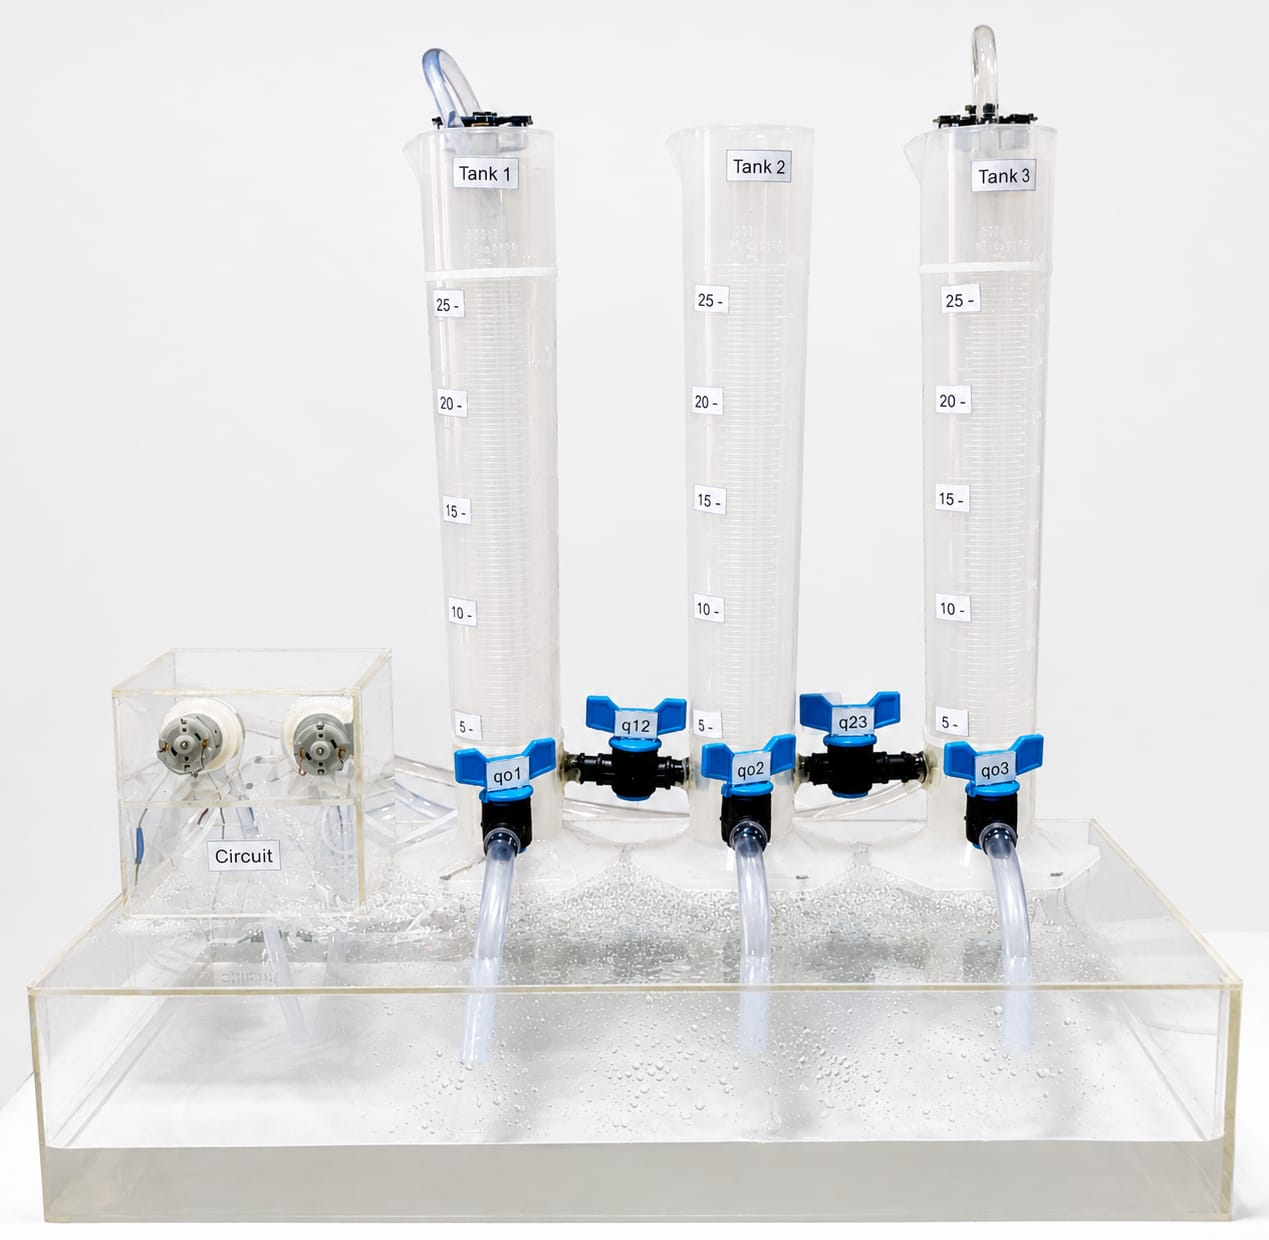
\includegraphics[width=\textwidth]{img/sistema.png}
    \caption{Planta física. Un vídeo demostrativo del funcionamiento de la planta
    está disponible en \url{https://www.youtube.com/watch?v=iw3A_h24A2c}.}
    \label{fig:sistema}
\end{figure}

La dinámica del sistema se obtiene por conservación de masa aplicada a cada depósito:

\begin{equation}
\frac{d}{dt}\begin{pmatrix}h_1\\h_2\\h_3\end{pmatrix}
= \frac{1}{A_{\mathrm{tank}}}
\begin{pmatrix}
q_{i1} - q_{12} - q_{o1}\\
q_{12} - q_{23} - q_{o2}\\
q_{i3} + q_{23} - q_{o3}
\end{pmatrix},
\label{eq:dinamica}
\end{equation}

donde $q_{oi}$ es el flujo de descarga del tanque $i$ y $q_{12}$, $q_{23}$ son los
flujos de acoplamiento. Los flujos de descarga se modelan por la expresión de
Torricelli $q_{oi} = \alpha_{oi}A_{oi}\sqrt{2g\,h_i}$, con $\alpha_{oi}$ el
coeficiente de descarga y $A_{oi}$ el área del orificio de salida. Los flujos de
acoplamiento admiten flujo bidireccional e incorporan una transición suave entre
regímenes laminar y turbulento mediante

\begin{equation}
q_{12}(h_1,h_2) = \alpha_{12}(h_1,h_2)\,A_{12}\sqrt{2g\,|h_1-h_2|}\,\operatorname{sgn}(h_1-h_2),
\end{equation}

donde el coeficiente dinámico $\alpha_{12}$ satura suavemente hacia el valor
turbulento $\alpha_{120}$ según

\begin{equation}
\alpha_{12}(h_1,h_2) = \alpha_{120}\tanh\!\left(\frac{2\,\lambda_{12}}{\lambda_{c12}}\right), \quad
\lambda_{12} = D_{12}\frac{\rho}{\eta}\sqrt{2g\,|h_1-h_2|},
\end{equation}

y de manera análoga para el acoplamiento entre los tanques 2 y 3, con coeficiente
turbulento $\alpha_{230}$, número de flujo crítico $\lambda_{c23}$ y diámetro
hidráulico $D_{23}$:

\begin{equation}
q_{23}(h_2,h_3) = \alpha_{23}(h_2,h_3)\,A_{23}\sqrt{2g\,|h_2-h_3|}\,\operatorname{sgn}(h_2-h_3),
\qquad
\alpha_{23} = \alpha_{230}\tanh\!\left(\frac{2\,\lambda_{23}}{\lambda_{c23}}\right).
\end{equation}

En notación compacta, el sistema se escribe en espacio de estados como

\begin{equation}
\dot{x}(t) = f\bigl(x(t),\,u(t)\bigr), \qquad y(t) = C\,x(t),
\label{eq:ss}
\end{equation}

donde $x = [h_1\;h_2\;h_3]^\top$, $u = [u_1\;u_3]^\top$, y la matriz de salida

\begin{equation}
C = \begin{bmatrix}1&0&0\\0&0&1\end{bmatrix}
\end{equation}

refleja el escenario de medición parcial en el que solo $h_1$ y $h_3$ son accesibles,
mientras que $h_2$ debe ser estimado. Los parámetros físicos de la planta, calibrados
experimentalmente mediante el procedimiento descrito en la
Sección~\ref{sec:metodologia}, se resumen en la Tabla~\ref{tab:parametros}.

\begin{table}[ht]
\centering
\caption{Parámetros físicos calibrados del sistema de tres tanques.}
\label{tab:parametros}
\begin{tabular}{llll}
\toprule
\textbf{Variable} & \textbf{Valor} & \textbf{Unidad} & \textbf{Descripción} \\
\midrule
$A_{\mathrm{tank}}$ & $3.02\times10^{-3}$ & m$^2$ & Área transversal de cada tanque \\
$\rho$       & 997     & kg/m$^3$  & Densidad del agua \\
$\eta$       & $8.9\times10^{-4}$ & Pa\,s & Viscosidad dinámica \\
$g$          & 9.81    & m/s$^2$   & Aceleración gravitacional \\
$\alpha_{o1,o2,o3}$ & 0.0271 & ---  & Coef.\ de descarga (calibrado, vaciado libre) \\
$D_{o1,o2,o3}$ & 10 & mm & Diámetro efectivo, orificios de salida (idéntico en los tres tanques) \\
$A_{o1,o2,o3}$ & $7.85\times10^{-5}$ & m$^2$ & Área efectiva, orificios de salida ($A_{oi}=\pi D_{oi}^2/4$) \\
$\alpha_{120}$ & 0.3038 & ---      & Coef.\ turbulento, acoplamiento 1--2 \\
$D_{12}$     & 10      & mm        & Diámetro hidráulico, acoplamiento 1--2 \\
$A_{12}$     & $7.85\times10^{-5}$ & m$^2$ & Área efectiva, acoplamiento 1--2 \\
$\lambda_{c12}$ & 24000 & ---      & Núm.\ de flujo crítico, acopl.\ 1--2 \\
$\alpha_{230}$ & 0.1344 & ---      & Coef.\ turbulento, acoplamiento 2--3 \\
$D_{23}$     & 10      & mm        & Diámetro hidráulico, acoplamiento 2--3 \\
$A_{23}$     & $7.85\times10^{-5}$ & m$^2$ & Área efectiva, acoplamiento 2--3 \\
$\lambda_{c23}$ & 29600 & ---      & Núm.\ de flujo crítico, acopl.\ 2--3 \\
$T_s$        & 2       & s         & Tiempo de muestreo \\
$q_{i1}^{\max}$ & $2.69\times10^{-5}$ & m$^3$/s & Flujo máximo de la bomba 1 \\
$q_{i3}^{\max}$ & $2.41\times10^{-5}$ & m$^3$/s & Flujo máximo de la bomba 2 \\
\bottomrule
\end{tabular}
\end{table}

Para fines de identificación, control y análisis de linealización, resulta necesario
caracterizar los puntos de equilibrio $(x_S, u_S)$ del sistema, es decir, las
ternas $(h_{1,S}, h_{2,S}, h_{3,S}, u_{1,S}, u_{3,S})$ que satisfacen
$f(x_S,u_S)=0$ para cada nivel de referencia $h_2^{\mathrm{ref}}$ de interés. Estos
puntos se obtienen resolviendo numéricamente el sistema de ecuaciones algebraicas no
lineales de la ecuación~\eqref{eq:dinamica} igualada a cero, mediante un algoritmo de
mínimos cuadrados no lineales con una penalización adicional que favorece soluciones
con $u_{3,S}\approx0$ cuando estas son factibles, dado que la bomba~3 no es
estrictamente necesaria para sostener los niveles de equilibrio en el rango de
operación considerado. Los puntos de equilibrio obtenidos con los parámetros
calibrados de la Tabla~\ref{tab:parametros} se presentan en la
Tabla~\ref{tab:puntos_operacion}.

\begin{table}[ht]
\centering
\caption{Puntos de operación calculados con los parámetros calibrados de la
Tabla~\ref{tab:parametros}, para distintas referencias de nivel en el tanque 2.}
\label{tab:puntos_operacion}
\begin{tabular}{ccccc}
\toprule
$h_2^{\mathrm{ref}}$ [m] & $h_{1,S}$ [m] & $h_{3,S}$ [m] & $u_{1,S}$ & $u_{3,S}$ \\
\midrule
0.10 & 0.1139 & 0.0818 & 0.3283 & 0.0012 \\
0.15 & 0.1675 & 0.1269 & 0.4029 & 0.0012 \\
0.20 & 0.2207 & 0.1727 & 0.4659 & 0.0012 \\
\bottomrule
\end{tabular}
\end{table}

Estos tres puntos de equilibrio coinciden con los tres niveles de la secuencia de
referencia escalonada utilizada en la validación experimental
($0.10 \rightarrow 0.20 \rightarrow 0.15$\,m, Sección~\ref{sec:resultados}), y son los
mismos empleados para inicializar el modelo de predicción (\textit{warm-start}) del
KoopmanMPC y del NMPC en cada cambio de referencia. Para $h_2^{\mathrm{ref}}=0.25$\,m
el algoritmo de búsqueda no logra converger a una solución físicamente admisible
dentro del rango operativo de la planta ($h_i \le 0.27$\,m considerando el margen de
saturación del integrador RK4), por lo que este nivel queda fuera del rango de
referencias evaluado experimentalmente.


%% ================================================================
\subsection{Linealización del Sistema No Lineal}
\label{sec:linealizacion}
%% ================================================================

Para contextualizar las limitaciones de los enfoques de control basados en
linealización local, mencionados en la Sección~\ref{sec:marco} como una de las
motivaciones del enfoque Koopman, y para disponer de una referencia cuantitativa
frente a la cual contrastar la representación global del modelo EDMD
(Sección~\ref{sec:koopman_edmd}), se presenta a continuación la linealización del
sistema no lineal~\eqref{eq:dinamica} alrededor de cada uno de los puntos de
equilibrio de la Tabla~\ref{tab:puntos_operacion}.

\subsubsection*{Jacobiano del sistema}

Dado el sistema no lineal $\dot{x} = f(x,u)$, su linealización de primer orden
alrededor de un punto de equilibrio $(x_S, u_S)$ tal que $f(x_S,u_S)=0$ está dada por

\begin{equation}
\Delta\dot{x} \approx A_{\mathrm{lin}}\,\Delta x + B_{\mathrm{lin}}\,\Delta u,
\qquad
A_{\mathrm{lin}} = \left.\frac{\partial f}{\partial x}\right|_{(x_S,u_S)}, \quad
B_{\mathrm{lin}} = \left.\frac{\partial f}{\partial u}\right|_{(x_S,u_S)},
\label{eq:jacobiano}
\end{equation}

donde $\Delta x = x - x_S$ y $\Delta u = u - u_S$ representan las desviaciones
respecto al equilibrio. La estructura de $A_{\mathrm{lin}}$ está determinada por las
derivadas parciales de los términos de Torricelli y de acoplamiento de la
ecuación~\eqref{eq:dinamica}. En particular, dado que
$\partial\sqrt{h}/\partial h = 1/(2\sqrt{h})$, la sensibilidad de los flujos de
descarga y de acoplamiento frente a variaciones del nivel crece de forma inversamente
proporcional a $\sqrt{h_S}$: a niveles de equilibrio bajos, las entradas
correspondientes del Jacobiano son mayores en valor absoluto, produciendo una
dinámica linealizada más rápida (polos más alejados del origen en el plano continuo)
que a niveles altos. Este efecto es la manifestación matemática directa de la
no linealidad de Torricelli, y constituye la razón por la cual ningún modelo
linealizado en un único punto de operación puede representar fielmente la dinámica
del sistema en todo su rango de trabajo.

\subsubsection*{Resultados de la linealización numérica}

El Jacobiano $A_{\mathrm{lin}}$ se calculó numéricamente por diferencias finitas
centrales alrededor de cada uno de los tres puntos de equilibrio de la
Tabla~\ref{tab:puntos_operacion}, utilizando los parámetros calibrados de la
Tabla~\ref{tab:parametros}. Para $h_2^{\mathrm{ref}}=0.10$\,m, el Jacobiano resultante
es

\begin{equation}
A_{\mathrm{lin}}^{(0.10)} =
\begin{bmatrix}
-0.1292 &  0.1246 &  0 \\
 0.1246 & -0.1751 &  0.0456 \\
 0 &  0.0456 & -0.0511
\end{bmatrix}\;\mathrm{s}^{-1},
\end{equation}

con autovalores continuos $\{-0.2841,\,-0.0662,\,-0.0050\}\,\mathrm{s}^{-1}$. El
autovalor de menor magnitud, $-0.0050\,\mathrm{s}^{-1}$, corresponde al modo más
lento del sistema y define la constante de tiempo dominante
$\tau_{\mathrm{dom}} = 1/0.0050 \approx 200$\,s. Este modo lento está asociado
físicamente al transporte de masa entre los tanques~2 y~3 a través del acoplamiento
de baja área efectiva, y es el responsable de la dinámica de respuesta lenta del
nivel $h_2$ observada experimentalmente. La Tabla~\ref{tab:linealizacion} resume
los autovalores continuos, la constante de tiempo dominante y los autovalores
discretos (obtenidos mediante $A_d=e^{A_{\mathrm{lin}}T_s}$ con $T_s=2$\,s) para
los tres puntos de operación considerados.

\begin{table}[ht]
\centering
\caption{Autovalores del sistema linealizado y constante de tiempo dominante en
cada punto de operación. $|\lambda_d|_{\max}$ es el módulo del autovalor discreto
dominante para $T_s=2$\,s.}
\label{tab:linealizacion}
\begin{tabular}{ccccc}
\toprule
$h_2^{\mathrm{ref}}$ [m] & Autovalores continuos [s$^{-1}$] & $\tau_{\mathrm{dom}}$ [s] & Autovalores discretos & $|\lambda_d|_{\max}$ \\
\midrule
0.10 & $-0.2841,\,-0.0662,\,-0.0050$ & 199.9 & $0.567,\,0.876,\,0.990$ & 0.990 \\
0.15 & $-0.2736,\,-0.0632,\,-0.0041$ & 245.5 & $0.579,\,0.881,\,0.992$ & 0.992 \\
0.20 & $-0.2651,\,-0.0610,\,-0.0035$ & 283.9 & $0.588,\,0.885,\,0.993$ & 0.993 \\
\bottomrule
\end{tabular}
\end{table}

\subsubsection*{Interpretación}

Tres observaciones se desprenden de la Tabla~\ref{tab:linealizacion}. En primer
lugar, los tres puntos de equilibrio son asintóticamente estables en lazo abierto,
ya que todos los autovalores continuos tienen parte real negativa (equivalentemente,
todos los autovalores discretos satisfacen $|\lambda_d|<1$); esto es consistente con
la naturaleza disipativa de un sistema hidráulico gravitacional sin retroalimentación
activa. En segundo lugar, la constante de tiempo dominante $\tau_{\mathrm{dom}}$
\emph{aumenta} de forma monótona con el nivel de operación, pasando de
$\approx200$\,s en $h_2^{\mathrm{ref}}=0.10$\,m a $\approx284$\,s en
$h_2^{\mathrm{ref}}=0.20$\,m, un incremento relativo del $42\%$. Esto significa que
una única linealización, calculada en cualquiera de estos puntos, subestimaría o
sobreestimaría sistemáticamente la velocidad de respuesta del sistema al desplazarse
hacia los otros niveles de operación, degradando el desempeño de cualquier
controlador o observador diseñado bajo el supuesto de invarianza del modelo
linealizado, tal como reporta la literatura para este tipo de plantas
\cite{tuwien2025}.

En tercer lugar, y de particular relevancia para esta investigación, el autovalor
discreto dominante $|\lambda_d|_{\max}$ se encuentra en todos los casos en el rango
$[0.990,\;0.993]$ para $T_s=2$\,s (Tabla~\ref{tab:linealizacion}), lo que corresponde a una dinámica \emph{marginalmente lenta}
en el sentido de que el modo dominante decae solo un $1\%$ por paso de muestreo. Esta
observación, obtenida aquí mediante la linealización clásica del modelo no lineal, es
consistente con el valor del radio espectral $\rho(\mathbf{A})=0.99990$ identificado
posteriormente para el modelo EDMD en el espacio de Koopman
(Sección~\ref{sec:metodologia}), y anticipa la limitación estructural del observador
de Luenberger que se caracteriza experimentalmente en la
Sección~\ref{sec:discusion}: con una dinámica dominante tan cercana al límite de
estabilidad marginal, la ganancia óptima del observador, obtenida mediante la
DARE, tiende a valores muy pequeños, ya que el propio modelo predice que el estado
no medido evoluciona casi sin amortiguamiento entre correcciones sucesivas.

Conviene notar que la linealización aquí presentada se basa en un único punto de
equilibrio por nivel de referencia y, por tanto, hereda las limitaciones señaladas:
es válida solo en un entorno reducido de dicho punto. El modelo EDMD adoptado en este
trabajo (Sección~\ref{sec:koopman_edmd}) busca precisamente superar esta limitación
mediante una representación lineal \emph{global}, identificada a partir de datos que
cubren la totalidad del rango de operación, sin sacrificar la linealidad del modelo
resultante.

%% ================================================================
\subsection{El Operador de Koopman y EDMD}
\label{sec:koopman_edmd}
%% ================================================================

Dado el sistema dinámico discreto $x_{k+1} = F(x_k, u_k)$, el operador de Koopman
$\mathcal{K}$ es un operador lineal infinito-dimensional que actúa sobre funciones
del estado denominadas \emph{observables}. Para una observable
$\varphi: \mathcal{X} \to \mathbb{R}$, el operador se define como:
\begin{equation}
\mathcal{K}\,\varphi(x) = \varphi(F(x,u)).
\end{equation}

La propiedad fundamental es que $\mathcal{K}$ es \emph{lineal en el espacio de
funciones}, aun cuando $F$ sea altamente no lineal~\cite{koopman1931,mezic2005}. Esta
propiedad contrasta con la linealización clásica discutida en la
Sección~\ref{sec:linealizacion}: mientras que el Jacobiano $A_{\mathrm{lin}}$ es una
aproximación local válida únicamente en un entorno del punto de equilibrio, el
operador de Koopman es \emph{exactamente} lineal, aunque de dimensión
infinita, para cualquier estado del sistema. La linealidad del operador permite
representar la evolución de cualquier observable como la acción de un operador
lineal, abriendo la puerta al uso de herramientas clásicas de control y
estimación~\cite{brunton2016,mauroy2020} sin las limitaciones de validez local que
exhibe la linealización punto a punto.

Si existe un subespacio finito de observables $\Phi(x) = [\phi_1(x),\ldots,\phi_N(x)]^\top$
invariante bajo $\mathcal{K}$, la evolución del sistema en el espacio elevado satisface
exactamente:
\begin{equation}
\Phi(x_{k+1}) = K\,\Phi(x_k) + B_\Phi\,u_k,
\label{eq:koopman_lineal}
\end{equation}

donde $K \in \mathbb{R}^{N\times N}$ y $B_\Phi \in \mathbb{R}^{N\times n_u}$ son
matrices constantes, es decir, \emph{independientes del punto de operación}, a
diferencia de $A_{\mathrm{lin}}$ y $B_{\mathrm{lin}}$ en la
ecuación~\eqref{eq:jacobiano}. En la práctica, la existencia de tal subespacio finito
no está garantizada para sistemas generales, pero puede construirse una aproximación
de alta calidad mediante el algoritmo EDMD~\cite{williams2015}. Dada una colección de
pares de datos $\{(x_j, x_j', u_j)\}_{j=1}^M$ con $x_j' = F(x_j, u_j)$, el EDMD resuelve
el problema de mínimos cuadrados:
\begin{equation}
K,\,B_\Phi = \arg\min \sum_{j=1}^{M} \bigl\|\Phi(x_j') - K\,\Phi(x_j) - B_\Phi\,u_j\bigr\|^2 + \lambda\|K\|_F^2,
\label{eq:edmd}
\end{equation}

donde $\lambda > 0$ es un parámetro de regularización de Tikhonov que mejora la
estabilidad numérica frente a problemas mal condicionados. La solución se obtiene
analíticamente mediante descomposición en valores singulares (SVD)~\cite{schmid2010}.
La calidad de la aproximación depende críticamente de la elección del diccionario
$\Phi$, siendo este uno de los principales retos metodológicos del enfoque
Koopman~\cite{garciarev2025}.

\paragraph{Elección del diccionario de observables.}
La selección de las funciones base $\phi_i$ debe balancear la expresividad del
diccionario con la estabilidad numérica del ajuste. Para sistemas con no
linealidades de tipo Torricelli, la literatura recomienda incluir términos raíz
cuadrada del estado, productos de pares de estados y los estados lineales
directamente medibles~\cite{korda2018, aponte2024}. Diccionarios más ricos
(polinomios de grado superior, funciones de base radial) pueden capturar dinámicas
más complejas, pero incrementan el riesgo de sobreajuste y
colinealidad~\cite{garciarev2025}. En el presente trabajo se adopta un diccionario de
8 observables informado por la física del sistema:
\begin{equation}
\Psi(\mathbf{x}) = \left[ \sqrt{h_1},\; \sqrt{h_2},\; \sqrt{h_3},\; h_1h_2,\; h_2h_3,\; h_1h_3,\; h_1,\; h_3 \right]^\top \in \mathbb{R}^8,
\label{eq:psi_dict}
\end{equation}

cuya justificación detallada, incluyendo el análisis de colinealidad que motivó la
exclusión de $h_2$ como término lineal, se desarrolla en la
Sección~\ref{sec:metodologia}. Los términos $\sqrt{h_i}$ encapsulan directamente la
no linealidad de Torricelli identificada en la
ecuación~\eqref{eq:dinamica}, mientras que los términos bilineales $h_ih_j$ capturan
la dependencia de los flujos de acoplamiento respecto al producto de niveles
adyacentes, además se incluyen los estados $h_1$  y $h_3$ que son estados medidos directamente del sistema.

\paragraph{Formalización mediante el teorema de Koopman.}
Bajo condiciones generales, el operador de Koopman posee un espectro compuesto por
autovalores y autofunciones que capturan la estructura geométrica de las órbitas del
sistema no lineal~\cite{mezic2005}. Brunton et al.~\cite{brunton2016} demostraron que
si se puede identificar un subespacio invariante finito de Koopman que contenga los
estados del sistema, entonces es posible transformar el control óptimo no lineal en
un problema LQR estándar. El EDMD actúa como una aproximación de la proyección $L^2$
del operador infinito-dimensional sobre el subespacio generado por
$\Phi$~\cite{williams2015}.

Una vez identificado el par $(K, B_\Phi)$, denotado $(\mathbf{A}, \mathbf{B})$ en el
resto de este documento, el modelo lineal~\eqref{eq:koopman_lineal} puede
utilizarse directamente para el diseño de controladores y observadores con
herramientas estándar del álgebra lineal, sin requerir linealizaciones locales
recalculadas en cada punto de operación~\cite{korda2018}. Esta es la propiedad
central que distingue al enfoque Koopman de la linealización clásica de la
Sección~\ref{sec:linealizacion}: un único par $(\mathbf{A},\mathbf{B})$, identificado
una sola vez a partir de datos que cubren todo el rango de operación, sustituye a la
familia de Jacobianos $\{A_{\mathrm{lin}}^{(h_2^{\mathrm{ref}})}\}$ que dependerían
del punto de equilibrio.


%% ================================================================
\subsection{Control Predictivo de Modelos (MPC) y su Formulación NMPC}
\label{sec:mpc_nmpc}
%% ================================================================

El control predictivo de modelos es una estrategia de control en lazo cerrado
que, en cada instante de muestreo, resuelve un problema de optimización sobre un
horizonte de predicción finito $N$~\cite{rawlings2009}. Para un sistema no lineal de
la forma~\eqref{eq:ss}, el NMPC minimiza la función de costo:

\begin{equation}
J_N = \sum_{n=1}^{N}\|\tilde{y}_n - y^{\mathrm{ref}}\|_q^2
+ \sum_{n=0}^{N-1}\!\Bigl(\|\tilde{u}_n\|_{R_1}^2 + \|\tilde{u}_n - \tilde{u}_{n-1}\|_{R_2}^2\Bigr),
\label{eq:nmpc_cost}
\end{equation}

sujeto a la dinámica del sistema $\tilde{x}_{n+1} = F(\tilde{x}_n, \tilde{u}_n)$ y las
restricciones de caja $x_{\min} \leq \tilde{x}_n \leq x_{\max}$,
$u_{\min} \leq \tilde{u}_n \leq u_{\max}$. El primer término penaliza el error de
seguimiento de la referencia de salida, mientras que el segundo suaviza las
variaciones de la señal de control y limita el esfuerzo actuador.

La resolución del NMPC requiere resolver~\eqref{eq:nmpc_cost} en cada paso de
muestreo mediante un solver de optimización no lineal. En este trabajo se emplea
IPOPT (Interior Point OPTimizer)~\cite{wachter2006} a través de la interfaz
CasADi~\cite{andersson2019}, con una estrategia de inicialización caliente
desplazada (\textit{shifted warm-start}) para reducir el tiempo de convergencia entre
pasos consecutivos. La integración del modelo de predicción se realiza mediante el
método de Runge-Kutta de cuarto orden (RK4) con paso $T_s = 2$\,s.

La principal ventaja del NMPC sobre los controladores lineales, incluyendo los
basados en la linealización de la Sección~\ref{sec:linealizacion}, es su capacidad
para manejar la no linealidad completa del sistema sin recurrir a linealización
local, lo que resulta en un seguimiento de referencia más preciso cuando el sistema
opera lejos del punto de equilibrio~\cite{rawlings2009, danai2022}. Sin embargo, esta
precisión tiene un costo computacional significativo: la resolución iterativa de un
programa no lineal en cada paso de muestreo puede ser prohibitiva para plataformas
embebidas con recursos limitados, motivando el desarrollo de alternativas como el
KoopmanMPC que conservan la precisión a menor costo.

\paragraph{Formulación del KoopmanMPC.}
El KoopmanMPC sustituye el modelo de predicción no lineal de~\eqref{eq:nmpc_cost} por
el modelo lineal en el espacio elevado~\eqref{eq:koopman_lineal}. En consecuencia, el
problema de optimización se convierte en un programa cuadrático (QP)
convexo~\cite{korda2018}:

\begin{equation}
\min_{\{\tilde{u}_n\}} \sum_{n=1}^{N} \|\tilde{z}_n - z^{\mathrm{ref}}\|_Q^2 + \sum_{n=0}^{N-1} \left( \|\tilde{u}_n\|_{R_1}^2 + \|\tilde{u}_n - \tilde{u}_{n-1}\|_{R_2}^2 \right),
\label{eq:koopman_mpc}
\end{equation}

sujeto a $\tilde{z}_{n+1} = \mathbf{A}\tilde{z}_n + \mathbf{B}\tilde{u}_n$,
$\tilde{z}_0 = \hat{z}_k$ (el estado elevado estimado), restricciones sobre $h_i$ y
$u_n$ transformadas al espacio de observables, y donde
$z^{\mathrm{ref}} = \Psi(x^{\mathrm{ref}})$ es la referencia en el espacio elevado. La
convexidad del problema~\eqref{eq:koopman_mpc} permite emplear solvers QP
especializados (en este trabajo, \texttt{sqpmethod} con factorización \texttt{qrqp}
de CasADi), que convergen de forma más eficiente y predecible que los solvers
NLP~\cite{korda2018, narasingam2019}, eliminando además la dependencia de un punto de
linealización que caracteriza a los controladores lineales clásicos.


%% ================================================================
\subsection{Observador de Luenberger}
\label{sec:luenberger}
%% ================================================================

Para sistemas lineales de la forma $x_{k+1} = Ax_k + Bu_k$, $y_k = Cx_k$, el
observador de Luenberger proporciona un estimado $\hat{x}_k$ mediante la corrección:

\begin{equation}
\hat{x}_{k+1} = A\hat{x}_k + Bu_k + L\bigl(y_k - C\hat{x}_k\bigr),
\label{eq:luenberger}
\end{equation}

donde $L \in \mathbb{R}^{n\times p}$ es la ganancia del observador. La dinámica del
error de estimación $e_k = x_k - \hat{x}_k$ satisface $e_{k+1} = (A - LC)\,e_k$, de
modo que el error converge asintóticamente a cero si y solo si todos los valores
propios de $(A - LC)$ se encuentran dentro del círculo unitario~\cite{rawlings2009}.

La clave de la propuesta de este trabajo es que, gracias al modelo lineal de
Koopman~\eqref{eq:koopman_lineal}, el diseño de Luenberger puede aplicarse
\emph{directamente} sobre la dinámica no lineal del sistema de tanques, trabajando en
el espacio de observables elevado, en lugar de requerir una linealización local como
la presentada en la Sección~\ref{sec:linealizacion}. Surana y
Banaszuk~\cite{surana2016} formalizaron esta idea para sistemas de control afín,
demostrando que las condiciones de observabilidad y la convergencia del error pueden
analizarse íntegramente en las coordenadas de Koopman. El procedimiento de diseño
adoptado en este trabajo utiliza la ecuación algebraica de Riccati discreta (DARE)
para obtener la ganancia óptima $L$, un enfoque numéricamente robusto respecto a
alternativas basadas en programación semidefinida~\cite{ye2025}:

\begin{equation}
L = \mathbf{A} X C^\top (C X C^\top + R)^{-1},
\label{eq:dare_gain_marco}
\end{equation}

donde $X$ es la solución única y definida positiva de la DARE:

\begin{equation}
\mathbf{A}^\top X \mathbf{A} - X - \mathbf{A}^\top X C^\top (C X C^\top + R)^{-1} C X \mathbf{A} + Q = 0.
\end{equation}

La calibración de $Q$ a partir de la covarianza empírica de los residuos de la
identificación EDMD, en lugar de una matriz identidad escalada, es una contribución
metodológica de este trabajo que se justifica y desarrolla en la
Sección~\ref{sec:metodologia}. Como se anticipó en la
Sección~\ref{sec:linealizacion}, el hecho de que el modo dominante del sistema, tanto
en su linealización clásica como en su representación EDMD, se encuentre muy cercano
al límite de estabilidad marginal ($|\lambda_d|_{\max}\approx0.99$--$0.9999$) tiene
implicaciones directas sobre la ganancia $L$ que produce la DARE, las cuales se
analizan en profundidad en la Sección~\ref{sec:discusion}.


%% ================================================================
\subsection{Filtro de Kalman Extendido (EKF)}
\label{sec:ekf_marco}
%% ================================================================

El EKF es la extensión más utilizada del filtro de Kalman óptimo para sistemas no
lineales. Propaga la estimación del estado y su covarianza mediante una
linealización local en cada paso de tiempo, es decir, recalculando en cada instante
un Jacobiano análogo al de la ecuación~\eqref{eq:jacobiano}, pero evaluado en el
estado estimado actual en lugar de en un punto de equilibrio fijo. La etapa de
predicción calcula:

\begin{equation}
\hat{x}_{k|k-1} = f(\hat{x}_{k-1|k-1},\, u_{k-1}), \qquad
P_{k|k-1} = F_k\,P_{k-1|k-1}\,F_k^\top + Q,
\label{eq:ekf_pred}
\end{equation}

donde $F_k = \partial f/\partial x\big|_{\hat{x}_{k-1|k-1}}$ es el Jacobiano de la
dinámica evaluado en el estimado actual y $Q$ es la covarianza del ruido de proceso.
La etapa de corrección actualiza el estimado con la medición disponible:

\begin{equation}
K_k = P_{k|k-1}H_k^\top\bigl(H_kP_{k|k-1}H_k^\top + R\bigr)^{-1}, \qquad
\hat{x}_{k|k} = \hat{x}_{k|k-1} + K_k\bigl(y_k - h(\hat{x}_{k|k-1})\bigr).
\label{eq:ekf_corr}
\end{equation}

La ganancia $K_k$ minimiza la traza de la covarianza del error bajo el supuesto de
que la linealización es una buena aproximación local, supuesto que puede violarse
significativamente en sistemas con no linealidades severas~\cite{surana2016}. Su
costo computacional, que requiere recalcular el Jacobiano $F_k$ en cada paso mediante
múltiples evaluaciones del modelo no lineal, constituye, como se muestra en la
Sección~\ref{sec:resultados}, el cuello de botella dominante del esquema EKF+MPC
sobre la planta física. El trabajo de Guo et al.~\cite{kiloekf2026} demostró que
reemplazar solo el modelo de medición del EKF por una representación elevada de
Koopman es suficiente para superar al EKF clásico, sugiriendo que el espacio de
observables es especialmente valioso en la etapa de corrección.


%% ================================================================
\subsection{Estimación por Horizonte Deslizante (MHE)}
\label{sec:mhe_marco}
%% ================================================================

El MHE es un enfoque de estimación basado en
optimización que generaliza el filtro de Kalman a sistemas no lineales con
restricciones~\cite{rawlings2009}. En cada instante de muestreo, el MHE resuelve un
problema de optimización sobre los últimos $N$ instantes, incorporando
explícitamente las restricciones físicas del estado:

\begin{equation}
J_N(k,\,(\tilde{x}_j)) = \|\tilde{x}_0 - \bar{x}_{k-N}\|_S^2
+ \sum_{j=0}^{N-1}\!\Bigl(\|\tilde{x}_{j+1} - F(\tilde{x}_j,u_{k-N+j})\|_Q^2
+ \|y_{k-N+j} - C\tilde{x}_j\|_R^2\Bigr),
\label{eq:mhe_cost}
\end{equation}

donde $\bar{x}_{k-N}$ es la estimación a priori del estado al inicio del horizonte,
$S$, $Q$ y $R$ son matrices de ponderación definidas positivas, y las variables de
decisión $\tilde{x}_j$ están sujetas a las restricciones
$x_{\min} \leq \tilde{x}_j \leq x_{\max}$. El primer término es el término de arribo
que penaliza la desviación respecto a la información a priori, mientras que el
segundo pondera las perturbaciones de proceso y el error de ajuste a las mediciones
disponibles.

El MHE es equivalente al filtro de Kalman cuando el sistema es lineal y los ruidos
son gaussianos, pero ofrece la ventaja adicional de manejar restricciones de forma
natural~\cite{rawlings2009}. Su principal limitación es el costo computacional
creciente con el horizonte $N$ y la no linealidad del modelo de proceso, lo que
dificulta su uso en plataformas con recursos limitados. Sin embargo, a diferencia del
observador de Luenberger de la Sección~\ref{sec:luenberger}, un estimador recursivo
de un solo paso, el MHE incorpora explícitamente una ventana de memoria de $N$
pasos, lo que le permite acumular evidencia sobre el estado no medido a lo largo del
tiempo y compensar, al menos parcialmente, los errores sistemáticos de modelo. Esta
diferencia estructural entre ambos estimadores es central para la interpretación de
los resultados experimentales presentados en la
Sección~\ref{sec:resultados} y discutidos en la
Sección~\ref{sec:discusion}. Netto y Mili~\cite{netto2020} demostraron que el
operador de Koopman puede integrarse con estimadores basados en optimización para
mejorar la precisión en presencia de no linealidades, mientras que Yin et
al.~\cite{yin2023} propusieron un MHE basado en datos con modelo de Koopman que
reduce el costo computacional respecto al MHE con modelo no lineal. La
implementación de MHE desarrollada en este trabajo sirve como línea base de
desempeño frente a la cual se compara el esquema Koopman completo.















\section{Metodología}
\label{sec:metodologia}

La investigación se desarrolló en seis etapas secuenciales que abarcan 
desde la construcción y calibración de la planta física hasta la 
validación experimental del esquema Koopman completo, incluyendo el 
diseño del observador, el controlador y el proceso iterativo de mejora 
que condujo a la versión final (v4). Cada etapa se describe a 
continuación con el nivel de detalle suficiente para garantizar la 
reproducibilidad de los resultados.

%% ================================================================
\subsection{Etapa 1: Revisión de la literatura y definición de brechas}
%% ================================================================

Se realizó una revisión sistemática del estado del arte en teoría del 
operador de Koopman, el método EDMD y su aplicación al control 
predictivo y a la estimación de estados, con especial atención a los 
trabajos fundacionales de Williams et al.~\cite{williams2015} sobre 
EDMD, de Korda y Mezić~\cite{korda2018} sobre control predictivo basado 
en Koopman, y de Surana y Banaszuk~\cite{surana2016} y Netto y 
Mili~\cite{netto2020} sobre observadores lineales en el espacio de 
Koopman. La revisión abarcó también los antecedentes experimentales más 
próximos al presente trabajo: el experimento en cuatro tanques de Aponte 
y Téllez-Castro~\cite{aponte2024}, la validación en simulación del 
KoopmanMPC para tres tanques de Hernández y 
Téllez-Castro~\cite{hernandez2026}, y la comparación experimental entre 
el observador de Koopman y el EKF documentada en el artículo en revisión 
en \textit{Sensors}~\cite{hernandez2025sensors}. Esta revisión permitió 
identificar con precisión las dos brechas que motivan la presente 
investigación: la ausencia de una validación experimental conjunta de 
observador y controlador Koopman en un sistema hidráulico con medición 
parcial operando en lazo cerrado, y la falta de una comparación 
cuantitativa rigurosa de dicho esquema frente al par MHE+NMPC sobre una 
planta física real.

%% ================================================================
\subsection{Etapa 2: Construcción y calibración de la planta física}
\label{sec:planta_fisica}
%% ================================================================

\subsubsection{Descripción mecánica e hidráulica}

La planta física consiste en tres tanques cilíndricos idénticos
fabricados a partir de tubo de PVC transparente de diámetro interior
nominal de $6.2$~cm, con una altura útil de $34$~cm y tapas herméticas
en ambos extremos. El área efectiva de sección transversal de cada
tanque, verificada geométricamente, es

\[
A_{\mathrm{tank}}=\pi(0.031)^2=3.02\times10^{-3}\;\mathrm{m}^2.
\]

Los tres tanques se disponen verticalmente sobre una estructura de soporte fabricada en acrílico transparente, diseñada específicamente para mantener los recipientes alineados y a la misma cota para que el flujo de acoplamiento entre tanques adyacentes
dependa exclusivamente de las diferencias de nivel hidrostático.

En la parte inferior de la planta se encuentra un depósito de
recirculación de acrílico, el cual actúa como reservorio hidráulico
común. El agua descargada por los tres tanques retorna por gravedad a
este depósito, desde donde es nuevamente impulsada hacia la planta,
permitiendo la operación continua en lazo cerrado sin necesidad de
alimentación externa de agua.

Los tanques 1 y 2, así como los tanques 2 y 3, se encuentran
interconectados mediante válvula de aguja que permite regular la apertura efectiva del drenaje identificadas como $q_{12}$ y $q_{23}$. Durante todos los experimentos
reportados en este trabajo, ambas válvulas se mantuvieron completamente
abiertas, de modo que la resistencia hidráulica asociada al flujo de
acoplamiento queda representada únicamente por los coeficientes
$\alpha_{120}$ y $\alpha_{230}$ del modelo dinámico descrito en la
ecuación~\eqref{eq:dinamica}.

Cada tanque dispone además de una salida inferior equipada con una
válvula de regulación identificada como $q_{o1}$, $q_{o2}$ y $q_{o3}$,
respectivamente. Estas válvulas permiten ajustar el área hidráulica
efectiva de drenaje y, para todos los experimentos realizados, se
mantuvieron en una posición fija y reproducible previamente determinada
durante el procedimiento de calibración experimental, definiendo así el
coeficiente de descarga $\alpha_o$ empleado en el modelo.

La recirculación del agua se realiza mediante dos bombas de diafragma
R385 alimentadas a $12$~V~DC, encargadas de suministrar caudal a los
tanques 1 y 3. Las bombas fueron seleccionadas por su bajo costo, su
robustez frente a operación prolongada bajo modulación PWM y su
comportamiento aproximadamente lineal en el rango de operación empleado.
El caudal máximo de cada bomba fue determinado experimentalmente como
parte del procedimiento de identificación de la planta.

En el costado izquierdo de la estructura se instaló un módulo de dos
niveles fabricado en acrílico. En el compartimento superior se alojan
las dos bombas de impulsión, mientras que en el compartimento inferior
se encuentra la electrónica de control, acondicionamiento de señales y
potencia utilizada para la instrumentación y accionamiento de la planta.

\subsubsection{Arquitectura electrónica de control}

El sistema de control embebido está construido alrededor de un 
microcontrolador ESP32 de 30 pines (núcleo dual Xtensa LX6 a 240~MHz, 
520~kB SRAM), elegido por su capacidad de procesamiento, su módulo 
Wi-Fi/Bluetooth integrado (no utilizado en este trabajo, pero disponible 
para extensiones futuras) y su compatibilidad con el entorno de 
programación Arduino, que facilita la lectura de los sensores ultrasónicos 
y la generación de señales PWM. El ESP32 cumple tres funciones 
simultáneas: adquirir las mediciones de los sensores ultrasónicos en los 
tanques~1,~2 y~3, generar las señales PWM de control hacia las bombas, y 
mantener la comunicación serie bidireccional con la computadora central 
que ejecuta los algoritmos de observación y control.

La medición del nivel en los tanques~1,~2 y~3 se realiza con sensores 
ultrasónicos HC-SR04, montados en la tapa superior de cada tanque con el 
haz acústico orientado verticalmente hacia la superficie libre del agua. 
El HC-SR04 opera a 5~V con un rango de medición de $2$ a $400$~cm y una 
resolución teórica de aproximadamente $3$~mm, determinada por la 
resolución temporal del temporizador interno del ESP32 ($1~\mu$s $\approx 
0.17$~mm por conversión de tiempo de vuelo). En condiciones estáticas, el 
ruido de medición observado fue de $\sigma \approx 2$~mm, consistente con 
las especificaciones del fabricante. El tanque~2 dispone de sensor, para hacer una comparación cuantitativa entre la estimación del observador y el valor real del nivel. Un filtro de rechazo de atípicos implementado en software 
descarta lecturas que difieran más de $5$~cm de la lectura inmediatamente 
anterior, eliminando los ecos espurios ocasionales que los HC-SR04 
producen cuando la superficie del agua está perturbada. Este filtro se 
aplicó de manera idéntica en todos los experimentos y para ambos métodos 
comparados.

El control de las bombas se implementa mediante un circuito de 
conmutación de potencia basado en el transistor MOSFET de canal N 
IRLZ44N, uno por cada bomba. El IRLZ44N fue seleccionado por su 
resistencia de encendido $R_{\mathrm{DS(on)}} \approx 22$~m$\Omega$ y 
por su tensión de umbral de compuerta $V_{GS(\mathrm{th})} \leq 2$~V, 
compatible con los niveles lógicos de 3.3~V del ESP32. El pin PWM del 
ESP32 se conecta a la compuerta del MOSFET a través de una resistencia 
serie de $100~\Omega$ que limita la corriente de carga de la capacidad de 
compuerta y reduce las oscilaciones de alta frecuencia en la conmutación. 
Una resistencia de $10~\mathrm{k}\Omega$ entre compuerta y fuente 
garantiza que el MOSFET permanece en corte durante el encendido y 
reinicio del microcontrolador, previniendo activaciones espurias de las 
bombas. La bobina inductiva de la bomba DC puede generar picos de tensión 
inversa (\textit{back-EMF}) al cortar la corriente; estos se suprimen 
mediante un diodo de rueda libre 1N4007 conectado en antiparalelo con los 
terminales de la bomba. Adicionalmente, un condensador electrolítico de 
$100~\mu$F se instala en paralelo con la alimentación de las bomba para 
desacoplar las perturbaciones transitorias de la fuente de alimentación de 
12~V. Las masas del ESP32 y del circuito de potencia son comunes, 
referenciadas al negativo de la fuente de 12~V. La frecuencia de la señal 
PWM se fijó en $1$~kHz, valor suficientemente alto para que la inercia 
mecánica y el caudal de la bomba promedien la señal efectivamente, 
evitando el fenómeno de caudal pulsante que se produce a frecuencias 
inferiores a $100$~Hz.


\begin{figure}[H]
    \centering
    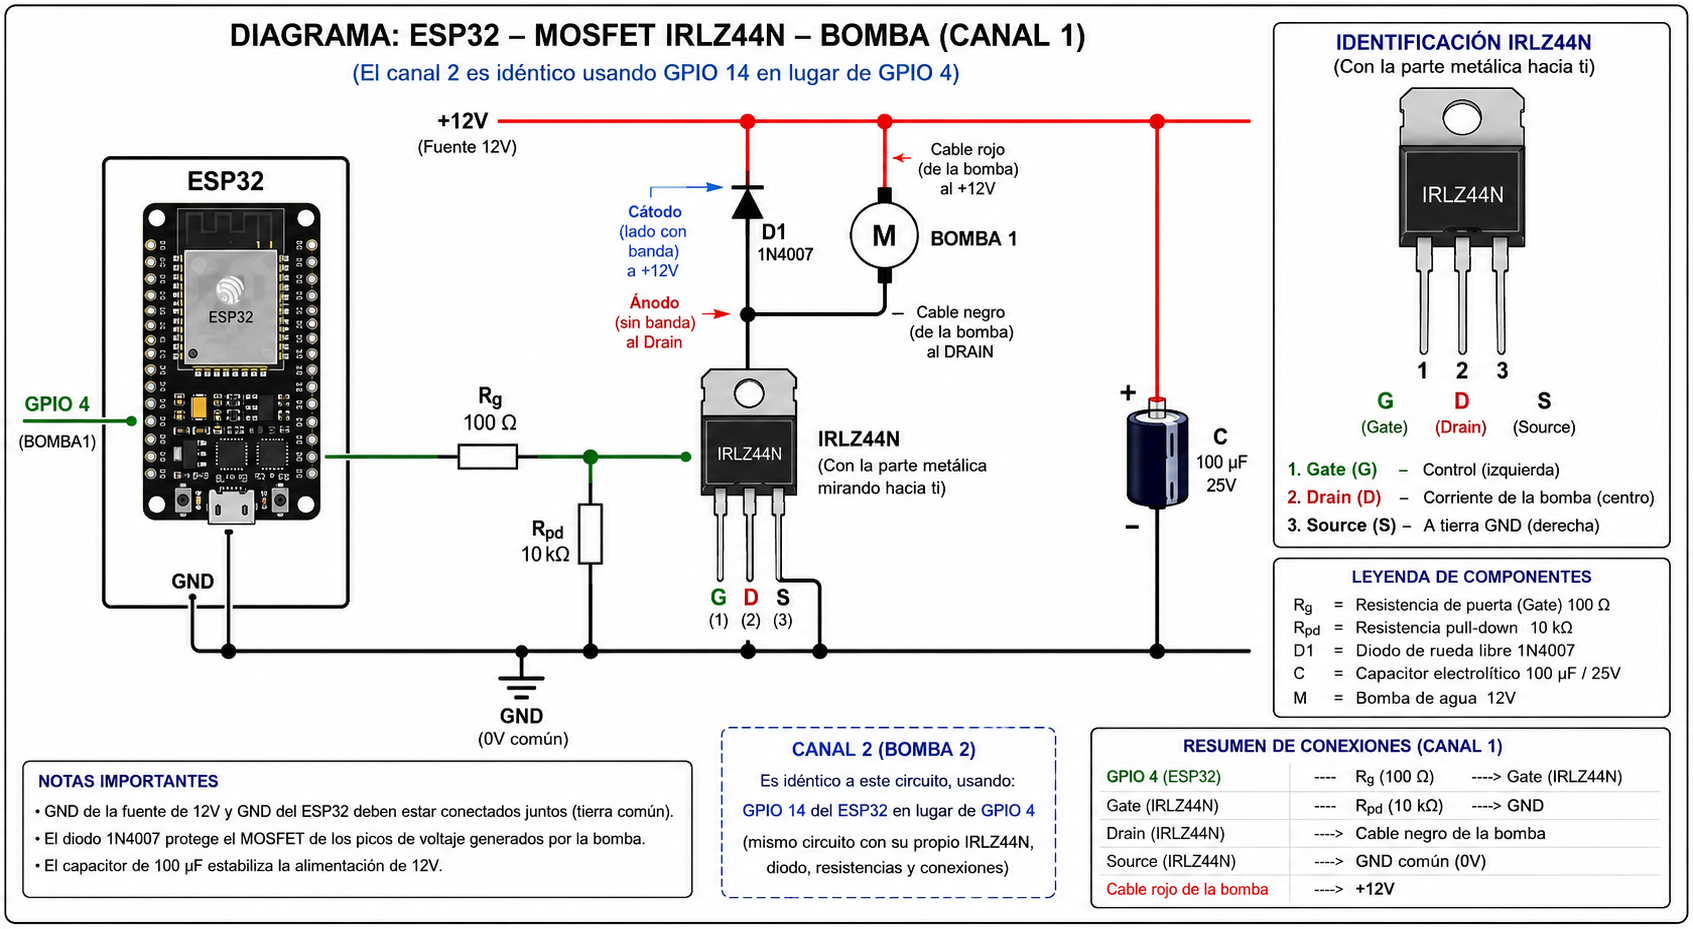
\includegraphics[width=\textwidth]{img/diagrama_bombas.png}
    \caption{Arquitectura electrónica de control.}
    \label{fig:electronica_control}
\end{figure}


La comunicación entre el ESP32 y la computadora central se realiza a 
través del puerto serie USB a $115200$~baudios. En cada ciclo de muestreo 
de $T_s = 2$~s, el ESP32 transmite una trama ASCII con el formato 
\texttt{h1\_m,h2\_m,h3\_m$\backslash$n}, donde \texttt{h1\_m} y 
\texttt{h3\_m} son los niveles medidos en metros con cuatro cifras 
decimales. El nivel del tanque~2 se transmite pero no influye en el lazo cerrado del esquema de control y observación; el campo central de la trama se reserva con valor cero 
para mantener la compatibilidad del parser. La computadora central 
responde con una trama \texttt{u1,u3$\backslash$n} que contiene los 
ciclos de trabajo normalizados $u_1, u_3 \in [0,1]$ con cuatro cifras 
decimales. El ESP32 aplica estos valores inmediatamente a los registros 
PWM que controlan los MOSFETs, completando el lazo de control. La latencia 
total de comunicación, medida experimentalmente, fue inferior a $15$~ms en 
el $99$\% de los ciclos, valor despreciable frente al periodo de muestreo 
de $2000$~ms.

\subsubsection{Procedimiento de calibración}
\label{sec:calibracion}

La calibración de los parámetros físicos de la planta se realizó mediante 
tres experimentos independientes, descritos a continuación en orden de 
ejecución.

\paragraph{Calibración del caudal máximo de las bombas.}
El caudal máximo de cada bomba se determinó conectando la salida de la 
bomba directamente a un recipiente graduado, aplicando el ciclo de trabajo 
máximo ($u = 1.0$, es decir, señal PWM al 100\%) durante $30$~s y 
midiendo el volumen recolectado. El ensayo se repitió tres veces por 
bomba; los valores medios obtenidos fueron $q_{i1}^{\max} = 2.69 \times 
10^{-5}$~m$^3$/s para la bomba~1 y $q_{i3}^{\max} = 2.41 \times 
10^{-5}$~m$^3$/s para la bomba~3. La diferencia de aproximadamente el 
10\% entre ambas bombas, aunque nominalmente idénticas, es habitual en 
componentes de bajo costo y refleja tolerancias de fabricación en los 
diafragmas y las válvulas de retención internas. Esta asimetría quedó 
reflejada en el parámetro de penalización del controlador $R_1(2,2) = 
1.0$ versus $R_1(1,1) = 0.1$, que penaliza diez veces más el uso de la 
bomba~3 dado su menor caudal máximo.

\paragraph{Calibración del coeficiente de descarga de los orificios de 
salida.}
El coeficiente de descarga $\alpha_o$ se determinó a partir de un ensayo 
de vaciado libre. Con las bombas apagadas y el tanque inicialmente lleno 
hasta $h = 0.15$~m, se registró el tiempo necesario para que el nivel 
descendiera hasta $h = 0.05$~m. La medición, repetida tres veces y 
promediada, arrojó un tiempo de vaciado de $\Delta t = 105$~s. El modelo 
de Torricelli para el vaciado libre de un tanque cilíndrico por un 
orificio de sección $A_o$ es:

\begin{equation}
A_{\mathrm{tank}}\,\frac{dh}{dt} = -\alpha_o A_o \sqrt{2g\,h},
\label{eq:vaciado}
\end{equation}

cuya integración analítica entre los niveles $h_i = 0.15$~m y $h_f = 
0.05$~m conduce a:

\begin{equation}
\alpha_o\,A_o = \frac{A_{\mathrm{tank}}\,2\!\left(\sqrt{h_i} - 
\sqrt{h_f}\right)}{\sqrt{2g}\,\Delta t}.
\label{eq:calibracion_ao}
\end{equation}

Sustituyendo los valores $A_{\mathrm{tank}} = 3.02 \times 10^{-3}$~m$^2$, 
$h_i = 0.15$~m, $h_f = 0.05$~m, $g = 9.81$~m/s$^2$ y $\Delta t = 
105$~s:

\begin{align}
\alpha_o\,A_o
  &= \frac{3.02\times10^{-3} \times 2\!\left(\sqrt{0.15}-\sqrt{0.05}\right)}
          {\sqrt{2 \times 9.81} \times 105} \notag \\
  &= \frac{3.02\times10^{-3} \times 2(0.3873 - 0.2236)}{4.429 \times 105}
   = \frac{9.890\times10^{-4}}{464.9}
   \approx 2.13\times10^{-6}~\mathrm{m}^{3}/(\mathrm{s}\cdot\mathrm{m}^{0.5}).
\end{align}

Dado que el diámetro del orificio de salida es $D_o = 10$~mm, el área 
nominal del orificio es $A_o = \pi D_o^2 / 4 = \pi(0.010)^2/4 = 7.85 
\times 10^{-5}$~m$^2$, y por tanto:

\begin{equation}
\alpha_o = \frac{2.13\times10^{-6}}{7.85\times10^{-5}} \approx 0.0271.
\label{eq:alphao_resultado}
\end{equation}

Este valor es significativamente inferior al coeficiente de descarga 
teórico típico para orificios de borde vivo ($\alpha_o \approx 0.61$), lo 
cual era esperable dado que las válvulas de aguja de la planta no están 
completamente abiertas: la apertura parcial de la válvula introduce una 
restricción adicional que reduce el caudal efectivo e impone un 
$\alpha_o$ efectivo mucho menor. El coeficiente $\alpha_o = 0.0271$ se 
aplicó de manera uniforme a los tres orificios de salida, dado que las 
tres válvulas de aguja se ajustaron a la misma posición de apertura y los 
ensayos de vaciado individual mostraron tiempos consistentes entre los 
tres tanques, con una desviación inferior al 3\%.

\paragraph{Identificación de los coeficientes de acoplamiento.}
Los coeficientes de acoplamiento turbulento $\alpha_{120}$ y $\alpha_{230}$ 
se tomaron de la literatura para sistemas de geometría análoga 
\cite{johansson2000, tuwien2025}, dado que las válvulas de bola que 
regulan el acoplamiento se operaron completamente abiertas durante todos 
los experimentos y la sensibilidad del modelo a pequeñas variaciones de 
estos coeficientes, en el rango de operación considerado, es menor que la 
sensibilidad al coeficiente de descarga $\alpha_o$. La validación del 
modelo calibrado se realizó comparando las trayectorias predichas por la 
integración RK4 del sistema~\eqref{eq:dinamica} con mediciones 
experimentales de respuesta escalón: el error de predicción a un paso 
fue inferior a $0.5$~mm para los niveles $h_1$ y $h_3$ en el rango 
$[0.05, 0.22]$~m, confirmando que el conjunto de parámetros de la 
Tabla~\ref{tab:parametros} representa fielmente la dinámica de la planta 
construida.

%% ================================================================
\subsection{Etapa 3: Identificación del modelo en el espacio de Koopman 
mediante EDMD}
\label{sec:edmd_ident}
%% ================================================================

\subsubsection{Selección del diccionario de observables}

La elección del diccionario $\Psi$ es el paso metodológico más crítico 
del enfoque EDMD, pues determina simultáneamente la expresividad del 
modelo lineal elevado y su condicionamiento numérico. Para el sistema de 
tres tanques, la estructura de la ecuación~\eqref{eq:dinamica} sugiere 
de manera natural la inclusión de términos $\sqrt{h_i}$, que encapsulan 
directamente la no linealidad de Torricelli, y de productos $h_i h_j$, 
que capturan la dependencia bilineal de los flujos de acoplamiento 
respecto al producto de niveles adyacentes. El análisis de colinealidad 
del conjunto de datos de entrenamiento mostró que incluir $h_2$ como 
término lineal independiente introduce una redundancia numérica severa 
con $(\sqrt{h_2})^2$, elevando el número de condición de la matriz de 
datos a valores superiores a $10^{12}$, lo que degrada la calidad de la 
regresión. Por este motivo, y dado que $h_2$ no es directamente medible 
y por tanto no puede usarse como observable de medición en el observador, 
se optó por omitir $h_2$ como término lineal y conservar únicamente $h_1$ 
y $h_3$, que sí son medibles. El diccionario resultante de ocho 
observables es:

\begin{equation}
\Psi(\mathbf{x}) = \left[ \sqrt{h_1},\; \sqrt{h_2},\; \sqrt{h_3},\; 
h_1 h_2,\; h_2 h_3,\; h_1 h_3,\; h_1,\; h_3 \right]^\top \in 
\mathbb{R}^8.
\label{eq:diccionario}
\end{equation}

\subsubsection{Generación de datos de entrenamiento}

Los datos de entrenamiento se generaron mediante integración numérica del 
modelo no lineal calibrado de la ecuación~\eqref{eq:dinamica} con paso 
$T_s = 2$~s, empleando un controlador proporcional de bajo desempeño que 
excita el sistema alrededor de distintos puntos de operación sin forzar 
la convergencia rápida hacia el equilibrio, con el fin de maximizar la 
diversidad de las trayectorias en el espacio de estados. El conjunto de 
entrenamiento se organizó en tres bloques de excitación complementarios. 
El primero comprende perturbaciones pequeñas, entre el $\pm 5\%$ y el 
$\pm 20\%$ del nivel nominal, alrededor de seis niveles de referencia 
distribuidos uniformemente entre $0.10$~m y $0.22$~m, cada uno con 
múltiples condiciones iniciales y perturbaciones aleatorias adicionales 
en la señal de control. El segundo bloque incluye perturbaciones grandes, 
de hasta el $\pm 40\%$ del nivel nominal, que cubren regímenes de 
operación alejados del punto de equilibrio donde la no linealidad de 
Torricelli es más pronunciada. El tercer bloque reproduce directamente 
los tránsitos del escenario experimental: $0.10 \rightarrow 0.20 
\rightarrow 0.15$~m, asegurando que el modelo EDMD ha sido entrenado con 
datos representativos de las condiciones que encontrará durante la 
validación. En total, el conjunto de entrenamiento comprende $8\,220$ 
pares $(z_k, u_k, z_{k+1})$, distribuidos de forma equilibrada entre los 
tres bloques de excitación.

\subsubsection{Regresión EDMD y estabilización espectral}

El problema de regresión EDMD se resuelve según la 
ecuación~\eqref{eq:edmd}, con regularización de Tikhonov 
$\lambda = 10^{-4}$, mediante la solución analítica por descomposición en 
valores singulares (SVD). El parámetro de regularización $\lambda = 
10^{-4}$ fue seleccionado mediante validación cruzada: valores más 
pequeños producen sobreajuste en las trayectorias de perturbación grande, 
mientras que valores superiores a $10^{-3}$ degradan la fidelidad del 
modelo en el régimen de perturbaciones pequeñas. Tras la regresión, se 
aplica una estabilización espectral que escala los autovalores de 
$\mathbf{A}$ cuyo módulo supera $1 - \delta$ hacia el valor $1 - \delta$, 
con $\delta = 10^{-4}$, garantizando que todos los autovalores de 
$\mathbf{A}$ satisfacen $|\lambda_i| \leq 1 - 10^{-4}$. Esta 
estabilización es esencial para el diseño del observador, dado que la 
DARE requiere que la matriz $\mathbf{A}$ no tenga autovalores fuera del 
disco unitario. El modelo resultante presenta un radio espectral 
$\rho(\mathbf{A}) = 0.9999$, consistente con las constantes de tiempo 
dominantes de $100$--$130$~s identificadas en la 
Tabla~\ref{tab:linealizacion}. El RMSE de predicción a un paso sobre un 
conjunto de validación independiente de $1\,500$ muestras no incluidas en 
el entrenamiento fue de $6.40 \times 10^{-5}$~m, equivalente a $0.064$~mm, 
confirmando una fidelidad de representación muy superior al nivel de ruido
de los sensores HC-SR04 ($\sigma \approx 2$~mm).

La Tabla~\ref{tab:edmd_props} resume las propiedades cuantitativas del
modelo EDMD identificado.

\begin{table}[H]
\centering
\caption{Propiedades del modelo EDMD identificado para el sistema de
tres tanques. Las muestras de entrenamiento corresponden a trayectorias
de bucle abierto con entradas PRBS; las de validación son trayectorias
independientes no utilizadas en el ajuste.}
\label{tab:edmd_props}
\begin{tabular}{lc}
\toprule
\textbf{Propiedad} & \textbf{Valor} \\
\midrule
Dimensión del diccionario $n_z$ & 8 \\
Muestras de entrenamiento & 8\,220 \\
Muestras de validación & 1\,500 \\
Regularización Tikhonov $\lambda$ & $10^{-4}$ \\
Umbral de estabilización $\delta$ & $10^{-4}$ \\
RMSE un paso (entrenamiento) & $9.74 \times 10^{-5}$~m \\
RMSE un paso (validación) & $6.40 \times 10^{-5}$~m \\
Radio espectral $\rho(\mathbf{A})$ & $0.9999$ \\
Rango de $|\lambda_i(\mathbf{A})|$ & $[0.0344,\;0.9999]$ \\
\bottomrule
\end{tabular}
\end{table}

El procedimiento EDMD produce las matrices $\mathbf{A} \in \mathbb{R}^{8\times8}$
y $\mathbf{B} \in \mathbb{R}^{8\times2}$ (6 cifras significativas), donde las
filas corresponden a los ocho observables
$[\sqrt{h_1},\sqrt{h_2},\sqrt{h_3},\;h_1h_2,\;h_2h_3,\;h_1h_3,\;h_1,\;h_3]^\top$
y las columnas de $\mathbf{B}$ a las entradas de las bombas $[u_1,\,u_3]^\top$:

\begin{equation}
\resizebox{\textwidth}{!}{$
\mathbf{A} =
\begin{bmatrix}
+0.7941 & +0.1507 & +0.0724 & +0.0216 & +0.0302 & +0.0344 & +0.0143 & -0.0942 \\
+0.1946 & +0.7226 & +0.0680 & +0.0548 & +0.0739 & -0.1497 & +0.0084 & +0.0127 \\
+0.0365 & +0.0833 & +0.8535 & +0.0173 & -0.0707 & -0.0142 & -0.0340 & +0.0932 \\
-0.0516 & +0.0113 & +0.0399 & +0.5721 & +0.3169 & +0.1792 & +0.1078 & -0.1236 \\
+0.0516 & +0.0042 & -0.0619 & +0.3049 & +0.3937 & +0.2134 & -0.1147 & +0.1401 \\
+0.0352 & -0.0175 & -0.0259 & +0.1833 & +0.1875 & +0.5980 & -0.0418 & +0.0639 \\
-0.0316 & +0.0987 & -0.0783 & +0.2436 & -0.0136 & -0.2643 & +0.8455 & +0.1724 \\
-0.0984 & +0.0471 & +0.0608 & -0.0872 & +0.1991 & -0.0421 & +0.1493 & +0.8004
\end{bmatrix}$},
\label{eq:A_matrix}
\end{equation}

\begin{equation}
\mathbf{B} =
\begin{bmatrix}
+1.938\times10^{-2} & -4.529\times10^{-4} \\
+2.296\times10^{-3} & +7.197\times10^{-4} \\
+6.218\times10^{-5} & +2.112\times10^{-2} \\
+2.855\times10^{-3} & +1.682\times10^{-4} \\
+2.549\times10^{-4} & +2.571\times10^{-3} \\
+2.193\times10^{-3} & +2.824\times10^{-3} \\
+1.591\times10^{-2} & -1.468\times10^{-4} \\
+6.298\times10^{-5} & +1.518\times10^{-2}
\end{bmatrix}.
\label{eq:B_matrix}
\end{equation}

La estructura de $\mathbf{A}$ es físicamente coherente: los
elementos diagonales ($0.572$--$0.999$) reflejan las dinámicas de
drenaje propias de cada tanque, mientras que los términos
fuera de la diagonal capturan el acoplamiento inter-tanque.
Todos los autovalores de $\mathbf{A}$ se encuentran estrictamente
dentro del disco unitario
($|\lambda|_{\max}=0.9999$, $|\lambda|_{\min}=0.0344$),
confirmando que el modelo lineal identificado es asintóticamente
estable en lazo abierto.
Las columnas de $\mathbf{B}$ muestran que la Bomba~1 ($u_1$)
excita principalmente los observables $\sqrt{h_1}$ y $h_1$
(filas 1 y 7), mientras que la Bomba~2 ($u_3$) excita
principalmente $\sqrt{h_3}$ y $h_3$ (filas 3 y 8), consistente
con la topología física del sistema.

%% ================================================================
\subsection{Etapa 4: Diseño del observador y del controlador}
\label{sec:diseno}
%% ================================================================

\subsubsection{Observador de Luenberger en el espacio de Koopman}

El diseño del observador parte de la representación lineal en el espacio 
elevado obtenida en la etapa anterior: $z_{k+1} = \mathbf{A} z_k + 
\mathbf{B} u_k + \varepsilon_k$, con $z_k = \Psi(x_k) \in \mathbb{R}^8$. 
La matriz de medición $C \in \mathbb{R}^{4 \times 8}$ selecciona las 
cuatro filas del vector de observables que corresponden a componentes 
directamente calculables a partir de las mediciones de los sensores 
HC-SR04: las filas 1, 3, 7 y 8 de $\Psi$, correspondientes a $\sqrt{h_1}$, 
$\sqrt{h_3}$, $h_1$ y $h_3$ respectivamente. Esta elección incluye tanto 
las formas lineales como las raíces cuadradas de los niveles medibles, lo 
que enriquece la información disponible para el observador respecto a 
utilizar únicamente los niveles lineales. La observabilidad del par 
$(\mathbf{A}, C)$ fue verificada numéricamente: el rango de la matriz de 
observabilidad discreta es $8$, igual a la dimensión del espacio elevado, 
confirmando que el estado $z_k$ es completamente observable a partir de 
la secuencia de mediciones disponibles.

La ganancia del observador $L \in \mathbb{R}^{8 \times 4}$ se obtiene 
resolviendo la ecuación algebraica de Riccati discreta (DARE), formulada 
en la forma dual al problema LQR de la ecuación~\eqref{eq:dare_gain_marco}. 
La elección de la matriz de ponderación $Q$ en la DARE tiene un impacto 
significativo sobre las propiedades del observador: un valor de $Q$ grande 
produce ganancias mayores y una convergencia más rápida, pero a costa de 
mayor amplificación del ruido de medición; un valor pequeño produce 
ganancias casi nulas y un estimador que opera principalmente como predictor 
abierto. Para determinar el valor óptimo de $Q$, se realizó un barrido 
sistemático sobre $Q = q I$ con $q \in \{0.01, 0.05, 0.1, 0.5, 1.0, 
5.0, 10.0\}$, evaluando en cada caso el polo dominante del observador 
$|\lambda|_{\max}(\mathbf{A} - LC)$ y la magnitud máxima de la ganancia 
$|L|_{\max}$. El valor $q = 0.1$, denominado ``Experimento A'' en la
nomenclatura de resultados, fue el que proporcionó el mejor equilibrio
entre velocidad de convergencia del error de estimación y sensibilidad al 
ruido de medición, con un polo dominante $|\lambda|_{\max}(\mathbf{A} -
LC) = 0.9402$ y una magnitud máxima de ganancia $|L|_{\max} = 0.558$.
Esta configuración fue utilizada en la totalidad de las corridas
experimentales del esquema Koopman v4 reportadas en este trabajo.

Cabe precisar que este resultado de la DARE corresponde al diseño
realizado directamente sobre la planta física, con la matriz $R$
ajustada a partir del ruido de medición real observado en los
sensores HC-SR04 ($\sigma \approx 2$~mm). En las pruebas de
estimación pura en simulación (Sección~\ref{sec:est_pura_sim}),
el mismo multiplicador nominal $q = 0.1$ se evaluó con $R$ ajustada
al ruido inyectado en el entorno de simulación ($\sigma = 1$~mm),
lo que produce una ganancia $L$ de distinta magnitud
($|L|_{\max} = 0.225$, polo dominante $= 0.950$) bajo el mismo
multiplicador $q$. Ambos resultados son, por tanto, diseños de
la DARE distintos, no inconsistentes, calibrados para
condiciones de ruido diferentes.

\subsubsection{Controlador KoopmanMPC con estado integrador}
\label{sec:koopmanmpc_v4}

El controlador KoopmanMPC se formula como el problema de optimización 
cuadrática de la ecuación~\eqref{eq:koopman_mpc}, con horizonte de 
predicción $N = 20$ y pesos de sintonía idénticos a los del NMPC de 
referencia: $q = 500$, $R_1 = \operatorname{diag}(0.1,\, 1.0)$ y $R_2 = 
\operatorname{diag}(0.1,\, 0.1)$. Esta identidad de parámetros entre 
ambos controladores es una condición metodológica indispensable para que 
la comparación experimental sea justa: cualquier diferencia de desempeño 
observada entre el esquema Koopman y el benchmark MHE+NMPC puede 
atribuirse exclusivamente a la estrategia de estimación y al modelo de 
predicción, no a diferencias en la agresividad del controlador. El peso 
terminal $w_N = 10$ se introduce en el último paso del horizonte para 
mejorar la estabilidad en lazo cerrado. El peso asimétrico $R_1(2,2) = 
1.0$ versus $R_1(1,1) = 0.1$ refleja el menor caudal máximo de la 
bomba~3 respecto a la bomba~1, penalizando más su uso para evitar que el 
controlador solicite flujos que la bomba no puede entregar.

Las primeras pruebas experimentales del esquema Koopman sin integrador 
revelaron la presencia de un sesgo negativo sistemático en estado 
estacionario, con valores de hasta $-0.288$~cm en la estimación de $h_2$, 
cuyo origen se analiza en detalle en la Sección~\ref{sec:discusion}. Para 
mitigar este sesgo sin alterar la naturaleza convexa del problema de 
optimización, se aumentó el vector de estado del MPC con una variable 
integradora escalar $z_{\mathrm{int}}$, definida por la dinámica discreta:

\begin{equation}
z_{\mathrm{int},k+1} = z_{\mathrm{int},k} + 
\bigl(h_2^{\mathrm{ref}} - \hat{h}_2^k\bigr)\,T_s,
\label{eq:integrador}
\end{equation}

donde $\hat{h}_2^k = (\hat{z}_{k,2})^2$ es la estimación del nivel del 
tanque~2 en el instante $k$, obtenida elevando al cuadrado el segundo 
componente del vector de estado de Koopman estimado. El estado aumentado 
del MPC es $\tilde{z} = [\Psi(\hat{x})^\top,\, z_{\mathrm{int}}]^\top 
\in \mathbb{R}^9$. La variable $z_{\mathrm{int}}$ se incluye en la 
función de costo del MPC con peso $k_i = 50$, lo que penaliza la 
acumulación de error de seguimiento y fuerza al controlador a corregir 
el sesgo de forma gradual en lugar de tolerarlo.

Con el fin de evitar la acumulación espuria del integrador durante los
transitorios de referencia, donde el error es de varios centímetros y
la integración sin restricción produciría una sobrecorrección severa al
alcanzar el nuevo nivel de referencia, se implementaron dos mecanismos
de gestión del integrador. El primero es una banda muerta (\textit{deadband}) 
de $3$~cm: la integración según la ecuación~\eqref{eq:integrador} solo se 
ejecuta cuando el error de seguimiento satisface $|h_2^{\mathrm{ref}} - 
\hat{h}_2^k| < 0.03$~m; fuera de este rango, $z_{\mathrm{int}}$ permanece 
congelado en su valor actual. Esta condición garantiza que el integrador 
actúe exclusivamente en el entorno del estado estacionario, donde su 
función de eliminación del sesgo es necesaria, y no durante los 
transitorios donde su acumulación sería perjudicial. El segundo mecanismo 
es una saturación de la variable integradora en el rango $\pm 0.03$~m$\cdot$s 
(\textit{anti-windup}), que limita la autoridad máxima del integrador 
incluso en presencia de errores persistentes, previniendo que una 
perturbación prolongada desestabilice el lazo de control. Adicionalmente, 
la variable $z_{\mathrm{int}}$ se reinicia a cero en el instante de cada 
cambio de referencia, evitando que el valor acumulado en el nivel anterior 
produzca una sobrecompensación inmediata en el nivel nuevo. Este reinicio
se aplica directamente a la variable de estado, no solo al punto de
inicio caliente (\textit{warm-start}) del optimizador, lo que
constituye una diferencia fundamental respecto a las versiones
anteriores del esquema (v1 a v3) que se documenta en la 
Tabla~\ref{tab:versiones_koopman}.

El problema de optimización aumentado se resuelve mediante el solver
\texttt{sqpmethod} de CasADi~\cite{andersson2019} con factorización
interna \texttt{qrqp}, inicializado mediante una estrategia de
\textit{warm-start} desplazado: al cambiar la referencia, el optimizador
se inicializa con el punto de equilibrio nominal correspondiente al nuevo
nivel de referencia, calculado resolviendo numéricamente el sistema
$f(x_S, u_S) = 0$ para el nuevo $h_2^{\mathrm{ref}}$; entre cambios de
referencia, se usa la solución óptima desplazada del paso anterior.

Adicionalmente, el esquema Koopman incorpora un prefiltro de
referencia en rampa que suaviza los cambios escalonados de
$h_2^{\mathrm{ref}}$ antes de ingresarlos como referencia al
KoopmanMPC, con el fin de evitar el sobreimpulso transitorio que
un escalón completo produce en el controlador con estado integrador
(véase la versión v1 sin esta suavización en la
Tabla~\ref{tab:versiones_koopman}). Esta rampa se aplicó de forma
asimétrica entre los dos esquemas comparados: el MHE+NMPC opera
sin suavización de referencia, recibiendo el escalón completo en
cada cambio. Esta decisión, evaluada experimentalmente en la
Sección~\ref{sec:lc_sim}, se justifica porque la incorporación de
la misma rampa al MHE+NMPC degrada su desempeño tanto en
simulación como en la planta física, de modo que cada esquema se
reporta en su configuración de mejor desempeño individual. Esta
asimetría afecta exclusivamente la comparación transitoria de la
Sección~\ref{sec:lc_sim} (simulación) y no contamina la
comparación experimental principal de la
Sección~\ref{sec:resultados_exp}, donde ambos esquemas reciben el
mismo escalón completo en la planta física.

%% ================================================================
\subsection{Etapa 5: Implementación de los esquemas de referencia}
\label{sec:benchmarks}
%% ================================================================

Para disponer de una línea base de comparación cuantitativa, se 
implementaron sobre el mismo modelo no lineal calibrado dos esquemas de 
referencia adicionales, con idénticos parámetros de horizonte y pesos de 
control. El primero y principal es el par MHE+NMPC, que representa el 
estándar del arte en control predictivo no lineal con estimación de 
estados bajo restricciones. El NMPC se formuló mediante la 
ecuación~\eqref{eq:nmpc_cost}, con el modelo de predicción integrado 
mediante RK4 con paso $T_s = 2$~s y resuelto en cada paso de muestreo 
con el solver IPOPT~\cite{wachter2006} a través de la interfaz 
CasADi~\cite{andersson2019}, utilizando una estrategia de 
\textit{warm-start} desplazado análoga a la del KoopmanMPC para reducir 
el tiempo de convergencia. El MHE se implementó sobre una ventana deslizante 
de $N_{\mathrm{MHE}} = 20$ pasos, minimizando la función de costo de la 
ecuación~\eqref{eq:mhe_cost} con el mismo solver IPOPT; las matrices de 
ponderación $Q_{\mathrm{MHE}}$, $R_{\mathrm{MHE}}$ y $S_{\mathrm{MHE}}$ 
se sintonizaron mediante el mismo procedimiento de barrido sistemático 
empleado para la ganancia del observador de Koopman, con el criterio de 
minimizar el RMSE de estimación de $h_2$ en un conjunto de validación 
en simulación.

El segundo esquema de referencia es el par EKF+KoopmanMPC, en el que un 
Filtro Extendido de Kalman sobre el modelo no lineal físico estima el 
vector de estado $\hat{x}_{k|k} \in \mathbb{R}^3$, que se eleva 
posteriormente al espacio de Koopman mediante la función $\Psi(\hat{x}_{k|k})$ 
antes de ser entregado al mismo KoopmanMPC. Este esquema fue objeto de una 
comparación experimental detallada en el artículo en revisión en 
\textit{Sensors}~\cite{hernandez2025sensors} y sirve aquí como referencia 
secundaria que permite aislar el efecto de la estrategia de estimación: 
dado que el controlador es idéntico en ambos casos, cualquier diferencia 
de desempeño entre EKF+KoopmanMPC y Koopman v4 se debe exclusivamente al 
observador.

%% ================================================================
\subsection{Etapa 6: Validación experimental y análisis de repetibilidad}
\label{sec:validacion}
%% ================================================================
La validación experimental se llevó a cabo sobre la planta física 
descrita en la Etapa 2, operando en lazo cerrado con comunicación serie 
entre el ESP32 y la computadora central. Se definió un escenario común de 
referencia escalonada para el nivel estimado del tanque~2, compuesto por 
tres segmentos: $h_2^{\mathrm{ref}} = 0.10$~m durante los primeros 
$264$~s, $h_2^{\mathrm{ref}} = 0.20$~m entre $264$~s y $528$~s, y 
$h_2^{\mathrm{ref}} = 0.15$~m entre $528$~s y $800$~s. Este escenario 
fue elegido por tres razones: cubre tanto transiciones ascendentes 
(+10~cm) como descendentes ($-$5~cm), los tres niveles de referencia 
coinciden con los puntos de equilibrio calculados en la 
Tabla~\ref{tab:puntos_operacion}, y el rango $[0.10, 0.20]$~m representa 
la zona de operación central de la planta donde el modelo EDMD fue 
entrenado con mayor densidad de muestras.
Para cada uno de los dos esquemas evaluados en la comparación principal,
Koopman v4 y MHE+NMPC, se ejecutaron cinco corridas experimentales
independientes bajo condiciones idénticas, para un total de diez 
experimentos de $800$~s de duración cada uno. Antes de cada corrida, los 
tres tanques se preacondicionaron llevando el nivel de $h_1$ y $h_3$ a 
valores cercanos al primer escalón de referencia ($h \approx 0.10$~m), y 
se verificó la estabilidad de las lecturas de los sensores ultrasónicos 
durante cinco ciclos consecutivos antes de activar el lazo de control. 
Los parámetros del observador y del controlador se mantuvieron fijos 
durante todas las corridas, sin resintonización entre experimentos.
Las métricas de desempeño se calcularon sobre el régimen permanente de 
cada corrida, definido como el conjunto de muestras con $t > 400$~s y 
excluyendo adicionalmente ventanas de $60$~s posteriores a cada cambio 
de referencia, para descartar el transitorio de asentamiento. Las 
métricas principales son el RMSE de seguimiento en estado estacionario 
$\mathrm{RMSE}_{\mathrm{SS}}$, el error absoluto medio (MAE), el sesgo 
(bias) y la desviación estándar del error en régimen permanente, todas 
ellas calculadas sobre el nivel estimado $\hat{h}_2$ respecto a la 
referencia $h_2^{\mathrm{ref}}$. La robustez de los resultados se evaluó 
mediante la dispersión de estas métricas entre las cinco corridas de cada 
método, cuantificada por la desviación estándar y el rango 
mínimo-máximo. Los tiempos de cómputo por paso se registraron con 
resolución de $1$~ms mediante el módulo \texttt{time} de Python, 
reportando la media y el percentil~99. Todo el código desarrollado, el
observador de Koopman, el KoopmanMPC v4, el MHE y el NMPC de
referencia, se gestionó en un repositorio público de GitHub
(\url{https://github.com/StevenHernandez88/koopman-three-tank-control}),
garantizando la trazabilidad de cada experimento y la reproducibilidad
de los resultados.

Es importante distinguir dos ventanas de régimen permanente
empleadas en este trabajo. La \emph{ventana global}, utilizada
para las métricas consolidadas de la Sección~\ref{sec:metricas_globales}
(Tabla~\ref{tab:cmp_exp}) y la comparación de estimación de $h_2$
(Tabla~\ref{tab:cmp_est_h2}), se define uniformemente como
$t > 400$~s excluyendo los $60$~s posteriores a cada cambio de
referencia, independientemente del segmento. La \emph{ventana
local por segmento}, utilizada para el desglose de la
Sección~\ref{sec:segmentos} (Tablas~\ref{tab:seg_rmse}
y~\ref{tab:seg_bias}), excluye en cambio los primeros $60$~s de
\emph{cada} segmento individual, lo que permite incluir el
Segmento~1 ($[0, 264]$~s), completamente anterior a $t = 400$~s
y por tanto ausente de la ventana global, en el análisis por
tramos. Ambas ventanas son métricas complementarias que responden
preguntas distintas (desempeño consolidado del experimento completo
versus desempeño específico de cada tramo de referencia), y no
deben interpretarse como un mismo valor desagregado de forma
inconsistente.

%% ================================================================
\section{Presupuesto}
\label{sec:presupuesto}
%% ================================================================

El anteproyecto original circunscribía la validación al entorno de simulación, por lo
que la totalidad de los recursos considerados en su presupuesto eran de acceso
abierto o de licencia institucional, sin costo directo. La construcción de la planta
física de laboratorio, que amplió el alcance del proyecto según se describe en la
Sección~\ref{sec:planta_fisica}, introdujo un rubro de componentes físicos que no
estaba contemplado originalmente. La Tabla~\ref{tab:presupuesto_software} resume los
recursos computacionales y de software empleados, y la Tabla~\ref{tab:presupuesto_planta}
detalla el costo de los componentes físicos adquiridos para la construcción de la
planta.

\begin{table}[H]
\centering
\caption{Recursos computacionales y de software.}
\label{tab:presupuesto_software}
\begin{tabular}{p{3.2cm}p{7cm}p{1.6cm}p{2.8cm}}
\toprule
\textbf{Rubro} & \textbf{Descripción y justificación} & \textbf{Valor (COP)} & \textbf{Fuente de financiación} \\
\midrule
Software científico (Python, NumPy, SciPy, CVXPY, Matplotlib) &
Herramientas de código abierto (licencia BSD/MIT), empleadas para la identificación
EDMD, el diseño del observador y del controlador, y las simulaciones comparativas. &
\$0 & Acceso abierto (\textit{open source}) \\
MATLAB/Simulink y CasADi + IPOPT &
MATLAB disponible mediante licencia estudiantil institucional de la Universidad
Distrital. CasADi e IPOPT son de acceso abierto. Empleados para los métodos de
referencia NMPC y MHE. &
\$0 & Licencia institucional UD / acceso abierto \\
Equipo de cómputo personal &
Computador personal del estudiante, con capacidad suficiente para las simulaciones y
para la comunicación en tiempo real con la planta física. No se requirió adquisición
de hardware de cómputo adicional. &
\$0 & Patrimonio personal del estudiante \\
Acceso a bases de datos científicas &
IEEE Xplore, Springer y Scopus mediante suscripción institucional de la UD,
complementado con arXiv y Google Scholar (acceso abierto). &
\$0 & Suscripción institucional UD / acceso abierto \\
Repositorio de código (GitHub) &
Repositorio público en GitHub para la gestión del código fuente, el control de
versiones y la reproducibilidad de los experimentos:
\url{https://github.com/StevenHernandez88/koopman-three-tank-control}. Gratuito
para proyectos de código abierto. &
\$0 & Acceso abierto (GitHub Free) \\
\bottomrule
\end{tabular}
\end{table}

\begin{table}[H]
\centering
\caption{Costo de los componentes físicos de la planta de laboratorio, adquiridos con
patrimonio personal del estudiante.}
\label{tab:presupuesto_planta}
\begin{tabular}{lr}
\toprule
\textbf{Componente} & \textbf{Valor (COP)} \\
\midrule
MOSFET & 16\,000 \\
Tanques & 84\,000 \\
Sensores ultrasónicos & 25\,000 \\
ESP32 & 32\,000 \\
Manguera & 5\,000 \\
Herramienta (broca) & 28\,000 \\
Bicomponente & 16\,000 \\
Base & 85\,000 \\
ESP32 (segunda unidad) & 15\,000 \\
Superpegante & 7\,000 \\
Transistores TIP41 & 6\,000 \\
Transistores 2N3904, resistencias, diodos & 7\,500 \\
Fuente 12\,V & 15\,000 \\
Bombas de agua & 28\,000 \\
Soportes de sensores & 12\,000 \\
Termoencogible & 3\,000 \\
Amarres & 1\,500 \\
Acrílico (bomba y circuito) & 25\,000 \\
Protoboard & 12\,000 \\
\midrule
\textbf{Total planta física} & \textbf{423\,000} \\
\bottomrule
\end{tabular}
\end{table}

El costo total del proyecto asciende, por tanto, a \$423.000 COP, correspondientes en
su totalidad a los componentes físicos de la planta y financiados con patrimonio
personal del estudiante; los recursos de software y de cómputo siguen sin representar
costo directo alguno. Esta cifra es consistente con la mencionada en la
Sección~\ref{sec:limitaciones} al discutir la accesibilidad económica de la
metodología.
























\section{Resultados}
\label{sec:resultados}

En esta sección se presentan los resultados de simulación y 
experimentales obtenidos para los esquemas de control y estimación 
evaluados. El escenario común de validación consiste en una 
trayectoria de referencia escalonada para el nivel del tanque~2 
con transiciones $0.10 \rightarrow 0.20 \rightarrow 0.15$~m, 
tiempo total $T = 800$~s, periodo de muestreo $T_s = 2$~s y ruido 
de medición intrínseco $\sigma \approx 2$~mm en los sensores 
HC-SR04. Todas las implementaciones se realizaron en Python con 
la plataforma CasADi~\cite{andersson2019}.

A lo largo de la sección se emplean las siguientes métricas de 
desempeño. El \textbf{RMSE de seguimiento en estado estacionario} 
($\mathrm{RMSE}_{\mathrm{SS}}$) se define como la raíz del error 
cuadrático medio de $\hat{h}_2 - h_2^{\mathrm{ref}}$ sobre el 
conjunto de muestras con $t > 400$~s, excluyendo ventanas de 
$60$~s inmediatamente posteriores a cada cambio de referencia 
para descartar el transitorio de asentamiento. El \textbf{RMSE 
transitorio} ($\mathrm{RMSE}_{\mathrm{tr}}$) se calcula sobre 
todas las muestras con $t > 400$~s sin excluir las ventanas de 
asentamiento, capturando el error durante los transitorios de 
referencia. El \textbf{error absoluto medio} (MAE) y el 
\textbf{sesgo} (bias) en régimen permanente complementan la 
caracterización escalar del desempeño; el sesgo es 
particularmente informativo porque cuantifica el error 
sistemático en estado estacionario, independientemente de su 
varianza. La \textbf{desviación estándar del error} 
($\sigma_{\mathrm{err}}$) cuantifica las fluctuaciones del 
error alrededor de su valor medio. Los \textbf{tiempos de 
cómputo} se reportan como la media y el percentil~99 (p99) 
del tiempo por paso, medidos con resolución de $1$~ms.

La presentación sigue una estructura progresiva: primero se
evalúan los componentes de forma aislada en simulación,
control puro con estado completo disponible y estimación
pura en lazo abierto, luego se integran en lazo cerrado
en simulación, y finalmente se presentan los resultados 
experimentales sobre la planta física.

%% ================================================================
\subsection{Resultados de Simulación}
\label{sec:resultados_sim}
%% ================================================================

Los resultados de esta subsección se obtuvieron ejecutando los 
algoritmos sobre el modelo no lineal calibrado de la 
ecuación~\eqref{eq:dinamica}, integrado con RK4 y paso 
$T_s = 2$~s, con ruido de medición gaussiano de desviación 
estándar $\sigma = 1$~mm añadido a las salidas $h_1$ y $h_3$
en cada paso de tiempo. El propósito es doble: verificar el
desempeño de cada componente en condiciones ideales, donde
el modelo de predicción y la planta son idénticos, y
establecer una cota superior de desempeño que sirva de
referencia para interpretar la degradación introducida por las 
discrepancias modelo--planta en los experimentos físicos.

\subsubsection{Control puro: NMPC frente a KoopmanMPC}
\label{sec:ctrl_puro_sim}

Con el fin de aislar el efecto del modelo de predicción 
independientemente de la estrategia de estimación, se asumió 
acceso completo al vector de estado $x_k = [h_1, h_2, 
h_3]^\top$ en cada instante de muestreo. El NMPC se implementó 
con horizonte $N = 20$, pesos $q = 500$, 
$R_1 = \operatorname{diag}(0.1, 1.0)$, 
$R_2 = \operatorname{diag}(0.1, 0.1)$ y peso terminal 
$w_N = 10$, resuelto con IPOPT/CasADi. El KoopmanMPC empleó 
los mismos parámetros, operando sobre el modelo EDMD de ocho 
observables%
\footnote{Este valor difiere del RMSE de $6.40\times10^{-5}$~m
reportado en la Tabla~\ref{tab:edmd_props}
(Sección~\ref{sec:edmd_ident}), que corresponde al conjunto de
validación general de $1\,500$ muestras aleatorias. El valor aquí
reportado se evalúa específicamente sobre la trayectoria de
validación cerrada $0.10\rightarrow0.20\rightarrow0.15$~m
utilizada en este experimento de control puro, cuyas excursiones
de mayor amplitud producen un error de predicción ligeramente
superior.}
con RMSE de predicción a un paso de
$8.62 \times 10^{-5}$~m sobre el conjunto de validación,
resuelto como programa cuadrático convexo con
\texttt{sqpmethod}/\texttt{qrqp} de CasADi.

\begin{figure}[H]
    \centering
    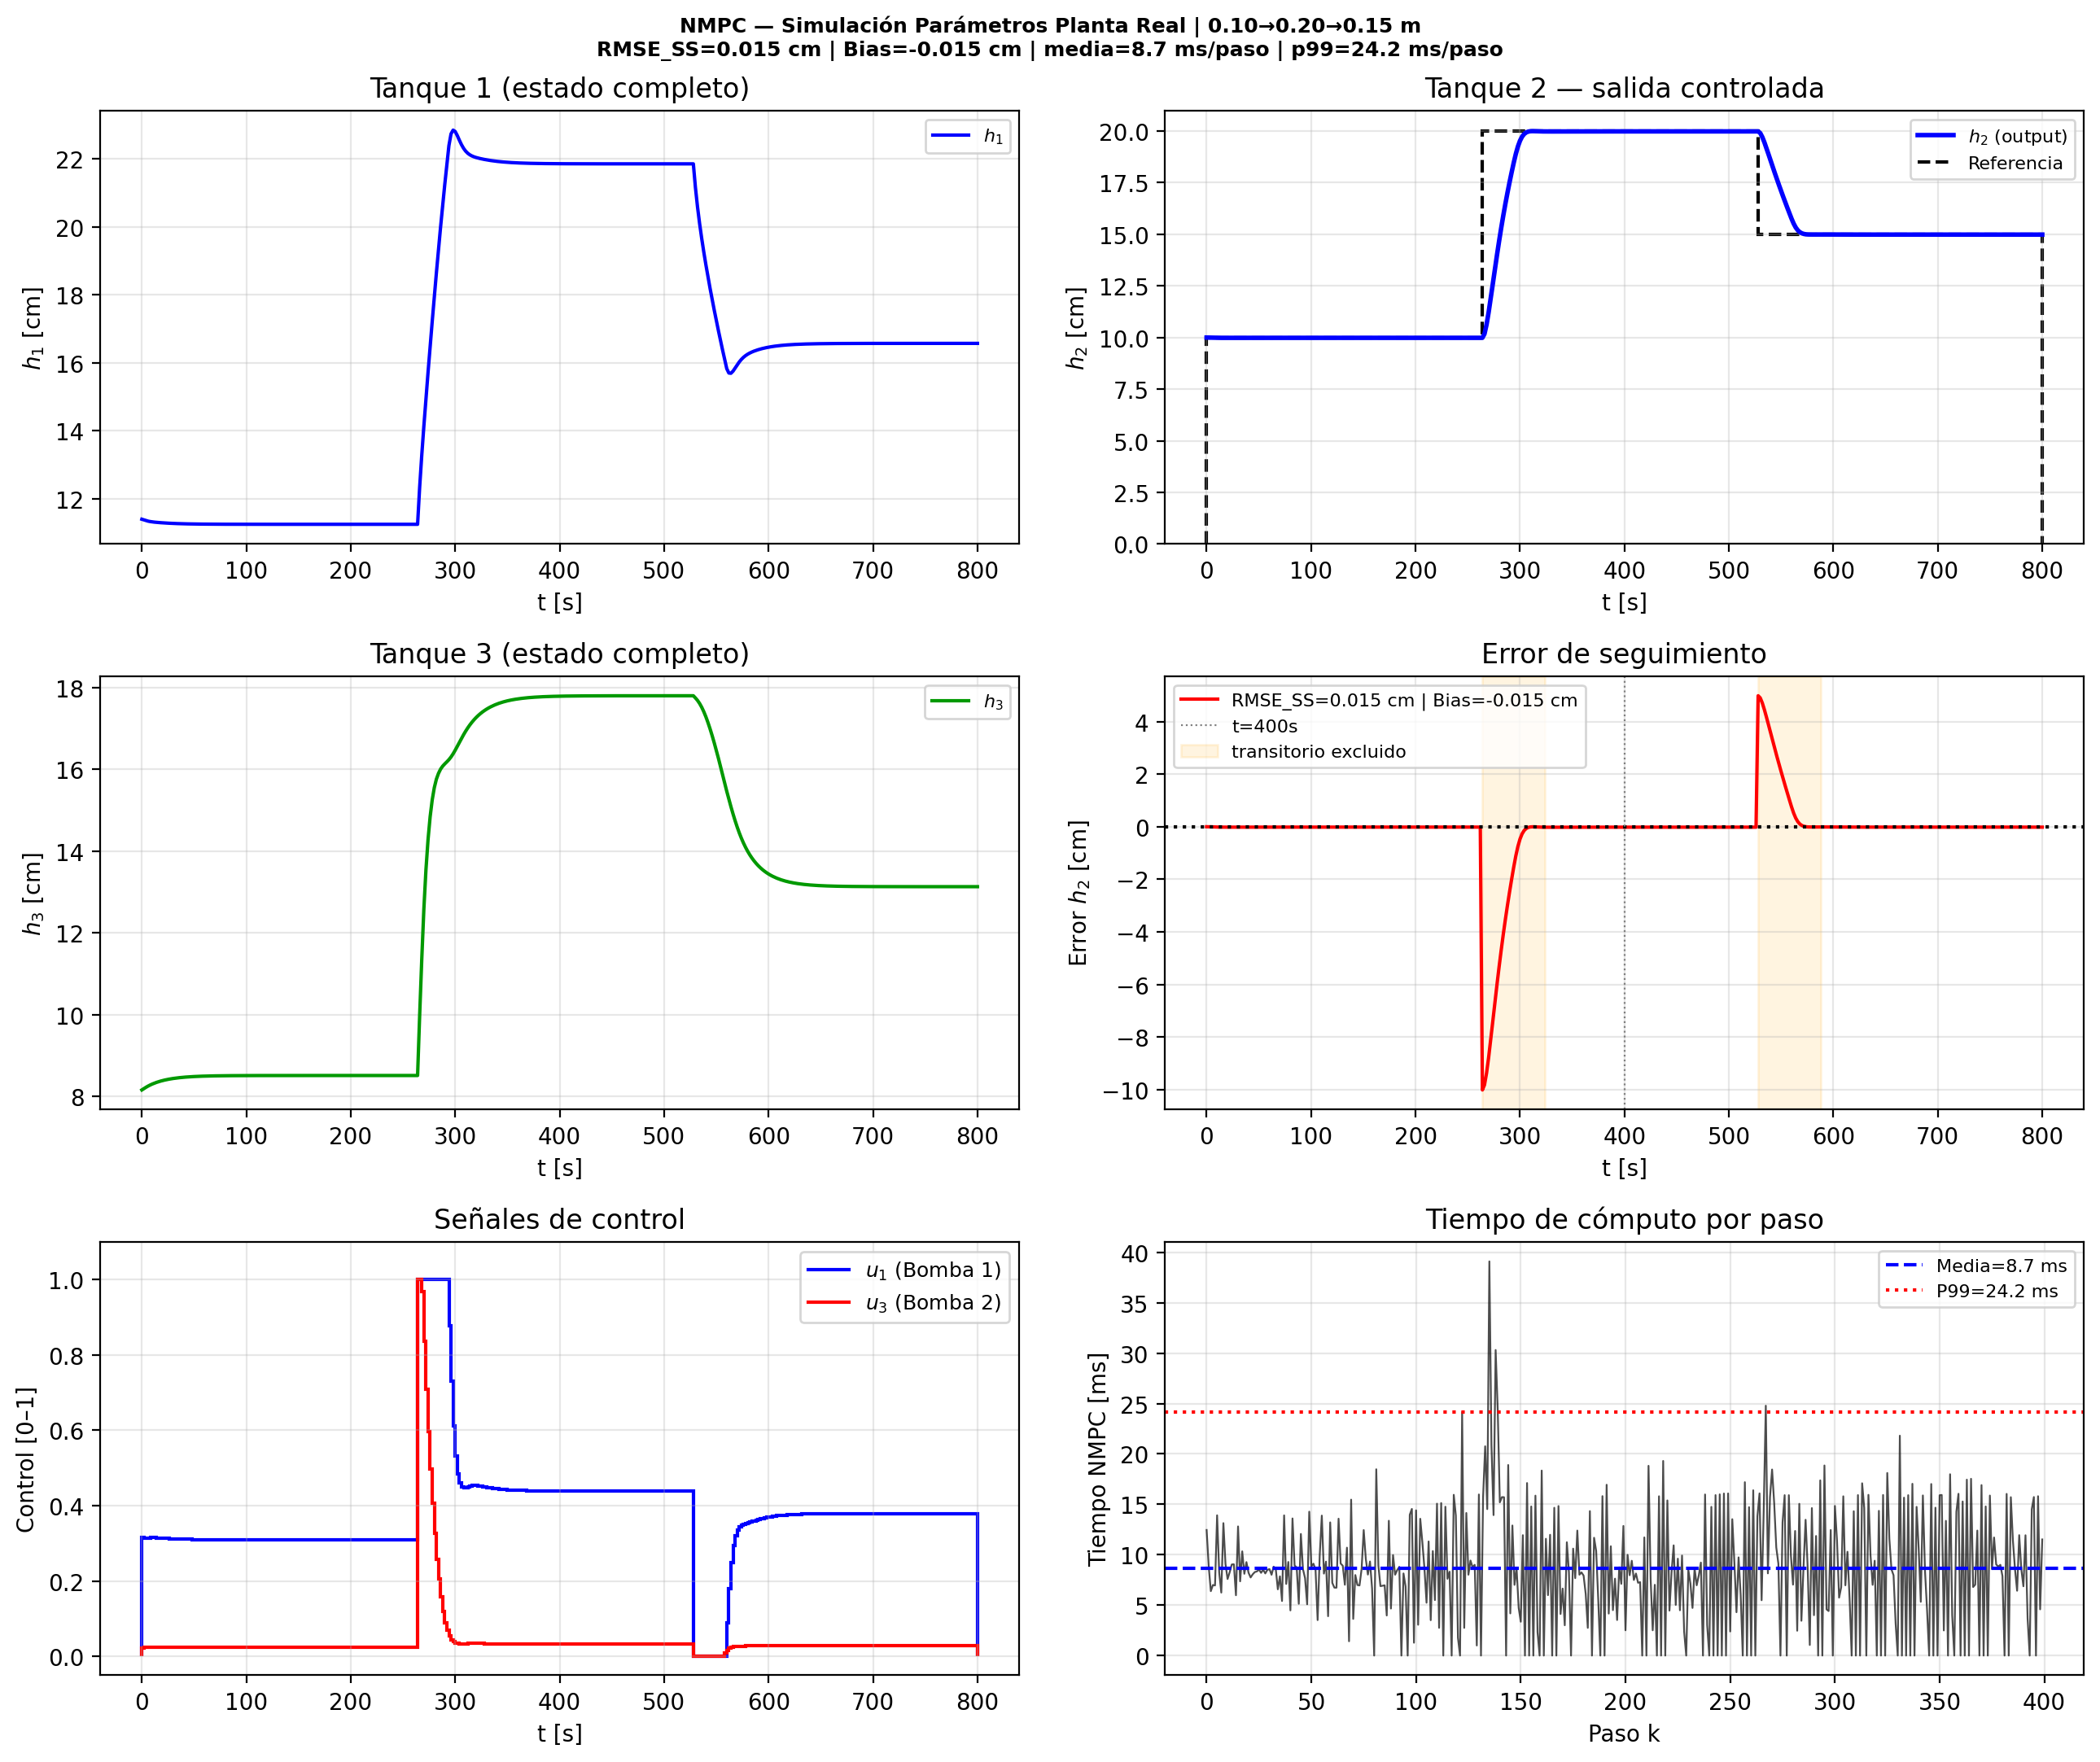
\includegraphics[width=\textwidth]{img/nmpc_planta_real.png}
    \caption{Trayectoria de seguimiento del NMPC en simulación 
    con estado completo disponible. 
    $\mathrm{RMSE}_{\mathrm{SS}} = 0.015$~cm,
    tiempo medio $= 8.7$~ms/paso.}
    \label{fig:nmpc_sim}
\end{figure}

\begin{figure}[H]
    \centering
    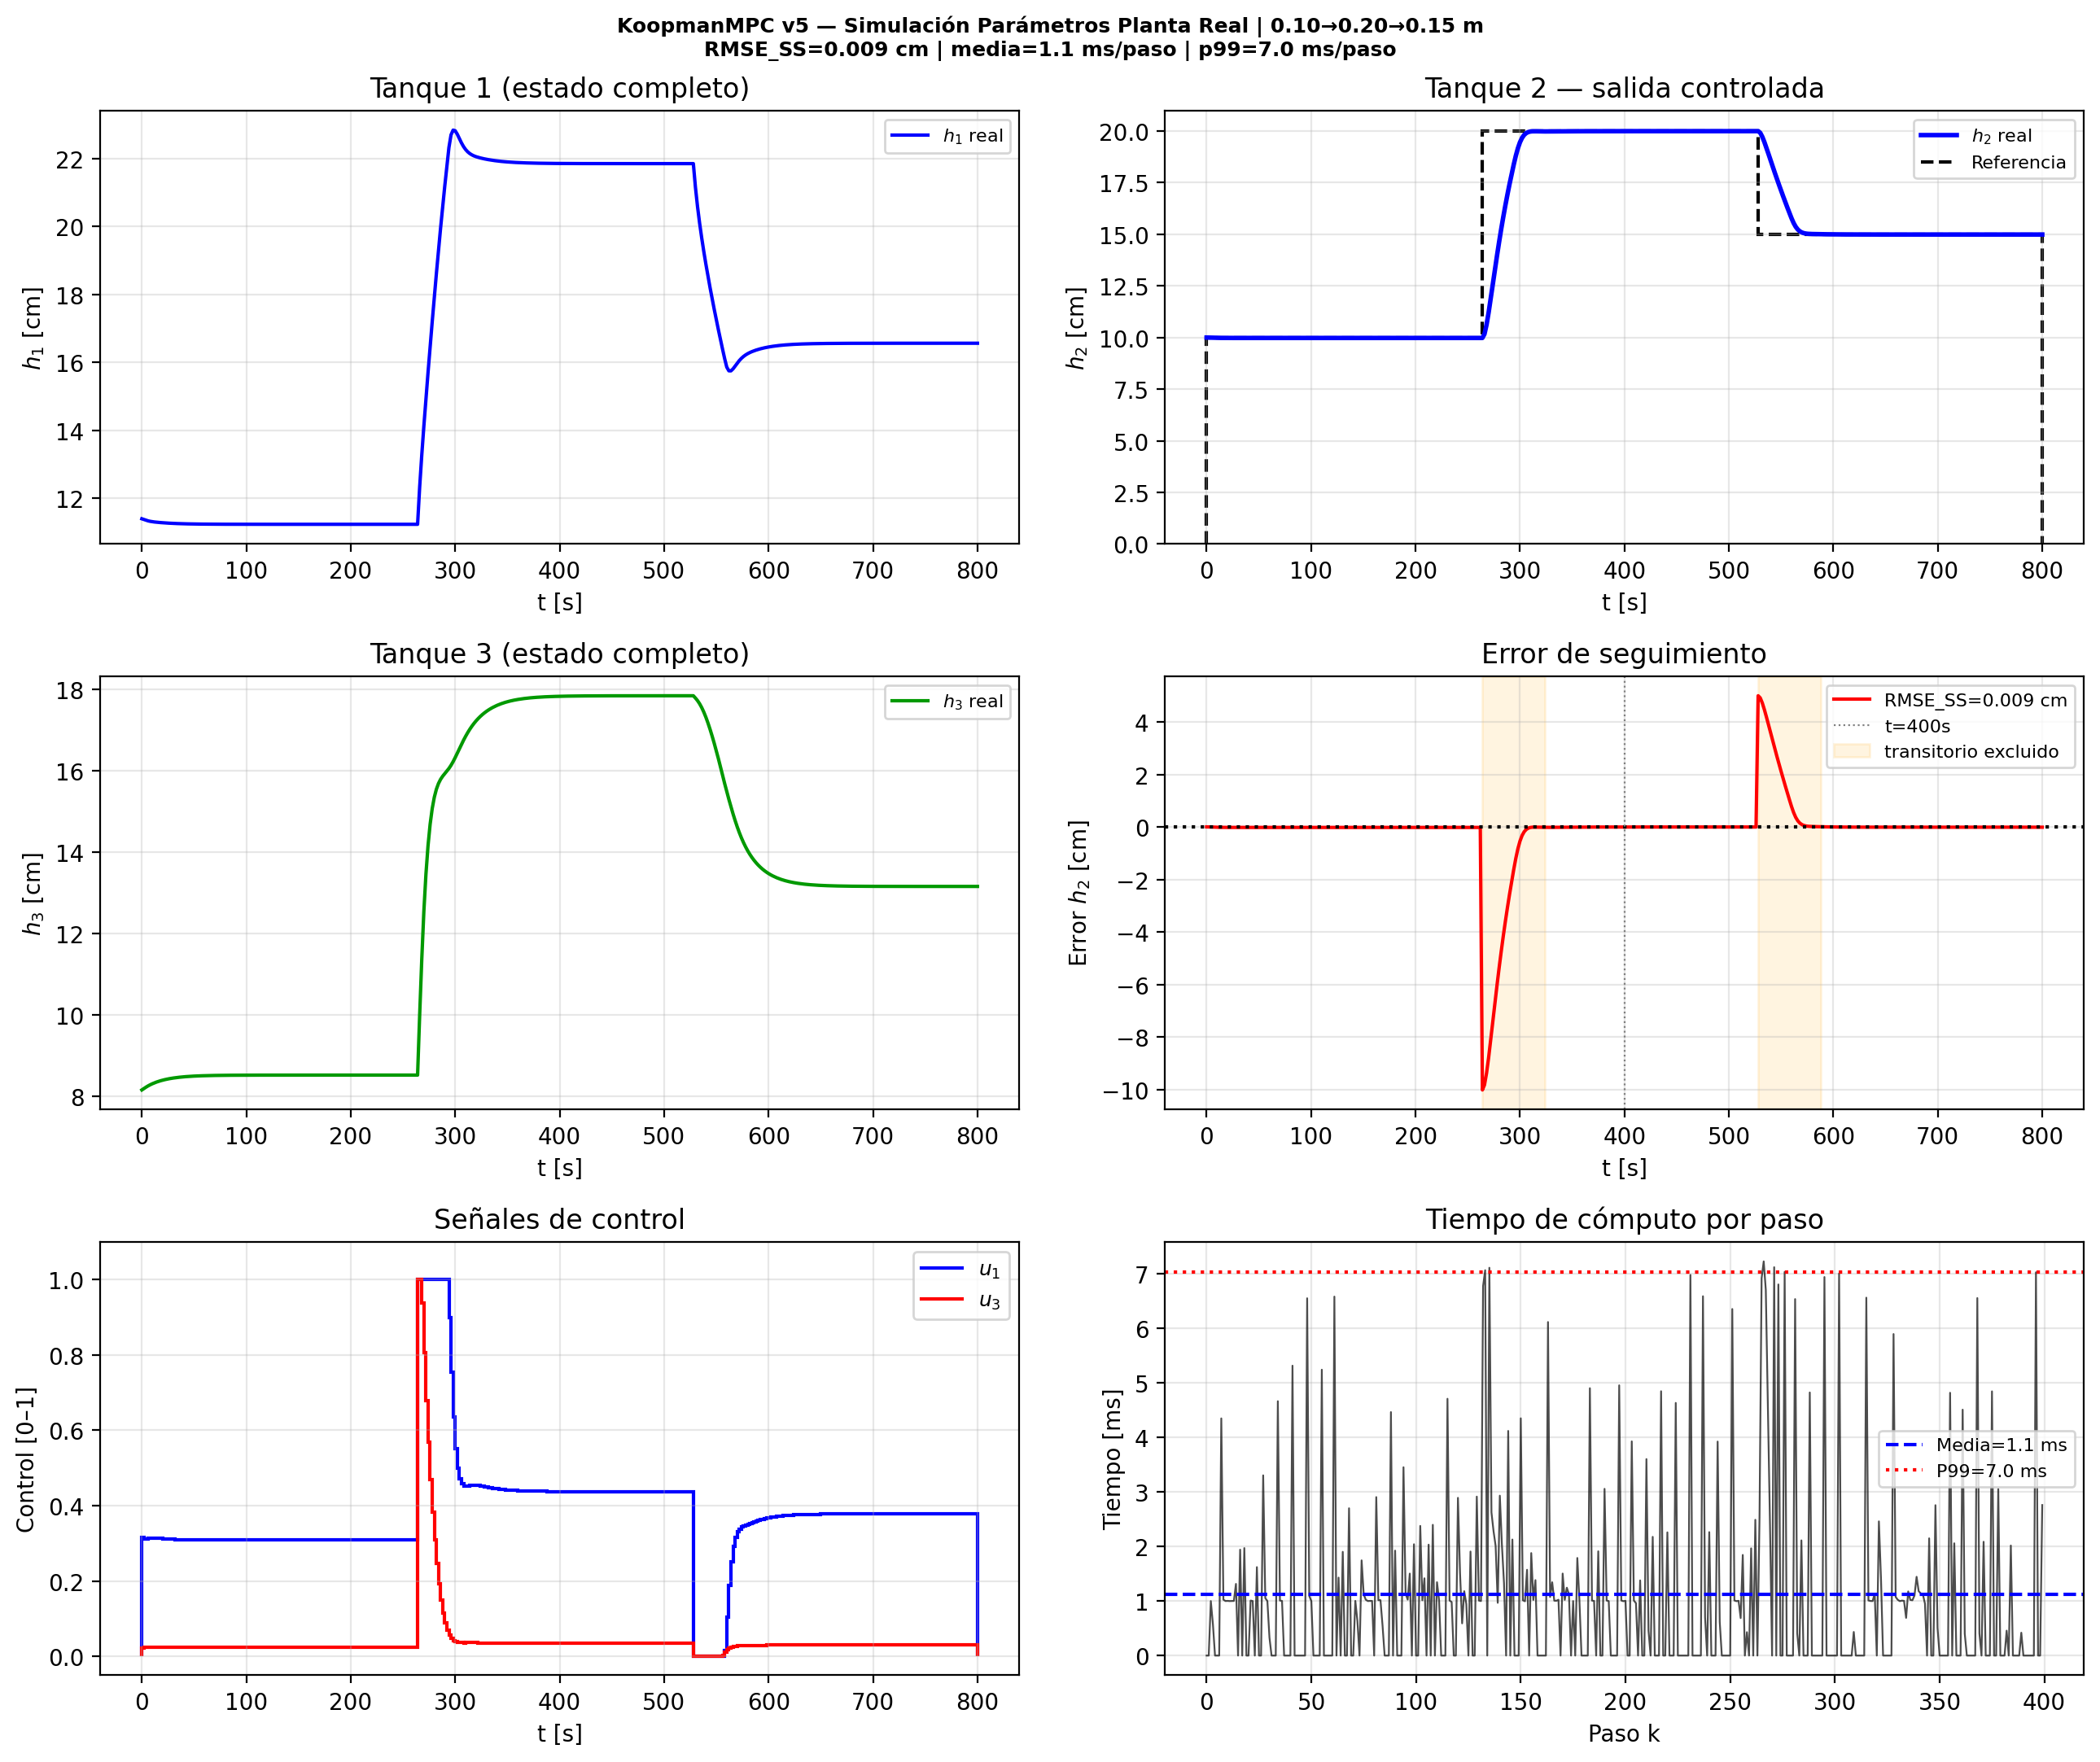
\includegraphics[width=\textwidth]{img/koopman_mpc_v5_planta_real.png}
    \caption{Trayectoria de seguimiento del KoopmanMPC en 
    simulación con estado completo disponible. 
    $\mathrm{RMSE}_{\mathrm{SS}} = 0.009$~cm, 
    tiempo medio $= 1.1$~ms/paso.}
    \label{fig:koopman_mpc_sim}
\end{figure}

\begin{table}[H]
\centering
\caption{Comparación en control puro (simulación, estado 
completo disponible, $N = 20$, $q = 500$, $\sigma = 1$~mm).}
\label{tab:cmp_ctrl_sim}
\begin{tabular}{lccc}
\toprule
\textbf{Métrica} & \textbf{NMPC} & \textbf{KoopmanMPC} & 
\textbf{Diferencia} \\
\midrule
$\mathrm{RMSE}_{\mathrm{SS}}$ [cm] & 0.015 & 0.009 & 
$-40\%$ (Koopman mejor) \\
Tiempo medio por paso [ms] & 8.7 & 1.1 &
$7.9\times$ más rápido \\
Tiempo p99 por paso [ms]   & 20.5 & 4.5 &
$4.6\times$ más rápido \\
\bottomrule
\end{tabular}
\end{table}

Las Figuras~\ref{fig:nmpc_sim} y~\ref{fig:koopman_mpc_sim} 
muestran las trayectorias de nivel estimado y referencia para 
ambos controladores; visualmente son prácticamente 
indistinguibles en la escala de la gráfica, lo que refleja 
que ambos logran un seguimiento sub-milimétrico en simulación. 
La Tabla~\ref{tab:cmp_ctrl_sim} cuantifica la comparación: el 
$\mathrm{RMSE}_{\mathrm{SS}}$ del KoopmanMPC es $0.009$~cm 
frente a $0.015$~cm del NMPC, una mejora del $40\%$. La 
ventaja más relevante desde el punto de vista práctico es la 
computacional: el KoopmanMPC es $7.9$ veces más rápido en
tiempo medio por paso ($1.1$~ms frente a $8.7$~ms) y $4.6$
veces más rápido en el percentil~99 ($4.5$~ms frente a
$20.5$~ms). Esta aceleración se explica por la reducción del 
problema de optimización de un programa no lineal (NLP), que 
IPOPT resuelve iterativamente mediante métodos de punto 
interior, a un programa cuadrático convexo (QP), que 
\texttt{sqpmethod} resuelve en muchas menos iteraciones con 
convergencia garantizada. El resultado valida la premisa 
central de Korda y Mezić~\cite{korda2018}: el modelo lineal 
en el espacio de Koopman permite recuperar la precisión de un 
controlador no lineal a una fracción de su costo computacional.

\subsubsection{Estimación pura: MHE frente al observador 
de Koopman}
\label{sec:est_pura_sim}

La comparación en estimación se realizó en lazo abierto: 
ambos estimadores recibieron como entrada la secuencia de 
señales de control del escenario de validación y las 
mediciones ruidosas de $h_1$ y $h_3$ generadas por el modelo 
calibrado. El MHE se configuró con horizonte 
$N_{\mathrm{MHE}} = 20$ pasos. El observador de Koopman 
utilizó la ganancia $L$ obtenida de la DARE con $Q = 0.1\,I$, 
que produce $|L|_{\max} = 0.225$ y polo dominante 
$|\lambda|_{\max}(\mathbf{A} - LC) = 0.950$.

\begin{figure}[H]
    \centering
    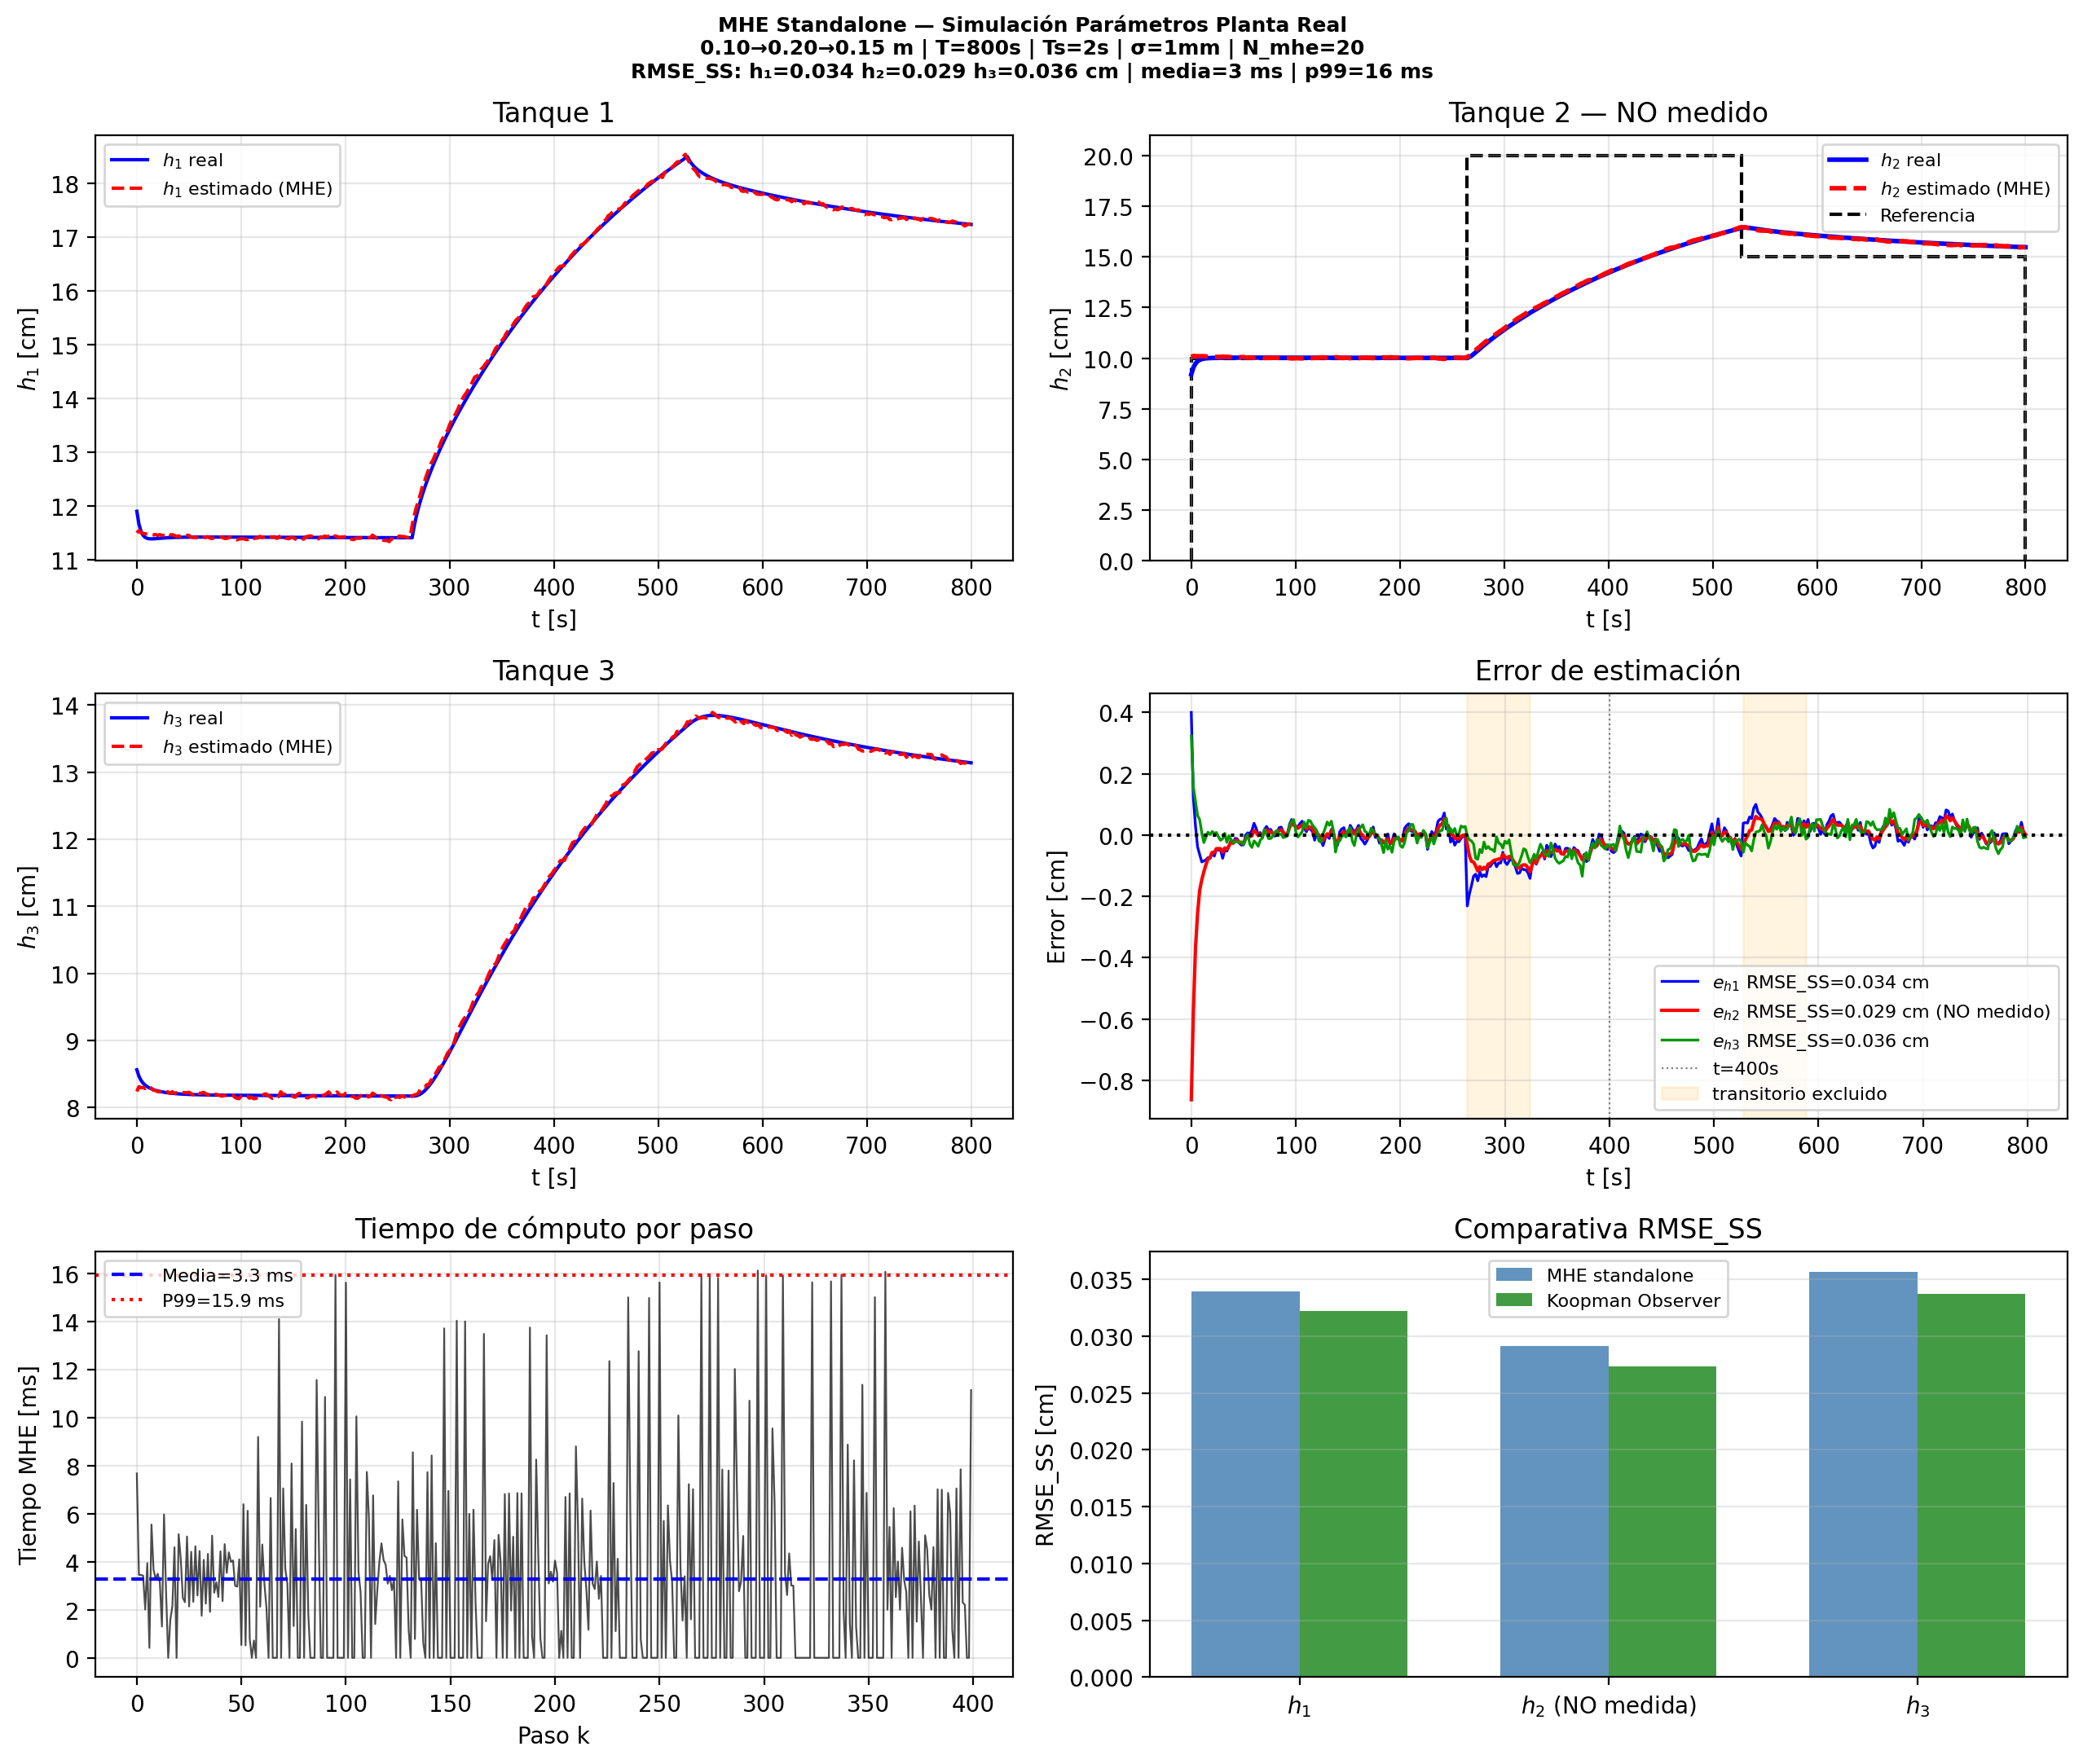
\includegraphics[width=\textwidth]{img/mhe_standalone_planta_real.png}
    \caption{Estimación en lazo abierto con MHE 
    ($N_{\mathrm{MHE}} = 20$, $\sigma = 1$~mm). 
    $\mathrm{RMSE}_{h_2} = 0.029$~cm.}
    \label{fig:mhe_sim}
\end{figure}

\begin{figure}[H]
    \centering
    \includegraphics[width=\textwidth]{img/koopman_observador_planta_real.png}
    \caption{Estimación en lazo abierto con el observador 
    de Koopman ($Q = 0.1\,I$, $|L|_{\max} = 0.225$, 
    $|\lambda|_{\max} = 0.950$). 
    $\mathrm{RMSE}_{h_2} = 0.026$~cm.}
    \label{fig:koop_obs_sim}
\end{figure}

\begin{table}[H]
\centering
\caption{Comparación en estimación pura (simulación, lazo 
abierto, $\sigma = 1$~mm en $h_1$ y $h_3$). Los valores de 
$h_1$ y $h_3$ corresponden al error de estimación respecto 
al estado real generado por el modelo; $h_2$ es la variable 
no medida de interés.}
\label{tab:cmp_est_sim}
\begin{tabular}{lccc}
\toprule
\textbf{RMSE [cm]} & \textbf{MHE} & 
\textbf{Observador Koopman} & \textbf{Diferencia} \\
\midrule
$h_1$ (medido)    & 0.034 & 0.032 & $-6\%$ (Koopman mejor) \\
$h_2$ (no medido) & 0.029 & 0.027 & $-7\%$ (Koopman mejor) \\
$h_3$ (medido)    & 0.036 & 0.034 & $-6\%$ (Koopman mejor) \\
\bottomrule
\end{tabular}
\end{table}

La Tabla~\ref{tab:cmp_est_sim} muestra que el observador de 
Koopman supera ligeramente al MHE en las tres variables de 
estado. El RMSE de $h_2$, la variable no medida de mayor 
interés, es $0.027$~cm para el observador de Koopman frente 
a $0.029$~cm para el MHE, una mejora del $7\%$. Este 
resultado tiene una interpretación precisa: cuando el modelo 
de predicción es exactamente la planta, el observador de 
Luenberger en el espacio de Koopman propaga la información 
de los estados medidos hacia el no medido a través de las 
correlaciones capturadas en la matriz $\mathbf{A}$, con una 
eficiencia comparable a la del MHE y un costo computacional 
despreciable frente a la optimización sobre ventana que este 
último requiere. La equivalencia en simulación establece que 
cualquier degradación que se observe en los experimentos 
sobre la planta física debe atribuirse a las discrepancias 
entre el modelo EDMD y la planta real, no a una inferioridad 
inherente del observador lineal.

\subsubsection{Lazo cerrado en simulación: MHE+NMPC frente 
al esquema Koopman}
\label{sec:lc_sim}

Una vez validados los componentes de forma aislada, se evaluó 
el desempeño de los dos esquemas completos en lazo cerrado 
sobre el modelo calibrado. El esquema Koopman integra el 
observador de Luenberger con la ganancia del Experimento A, 
el KoopmanMPC con $N = 20$ y pesos idénticos al NMPC, el 
estado integrador con peso $k_i = 50$, la \textit{deadband} 
de $3$~cm y la saturación \textit{anti-windup} en 
$\pm 0.03$~m$\cdot$s. El benchmark MHE+NMPC integra el MHE 
con $N_{\mathrm{MHE}} = 20$ y el NMPC con los mismos 
parámetros. Ambos esquemas se inicializan en el punto de 
equilibrio correspondiente a $h_2^{\mathrm{ref}} = 0.10$~m.

\begin{figure}[H]
    \centering
    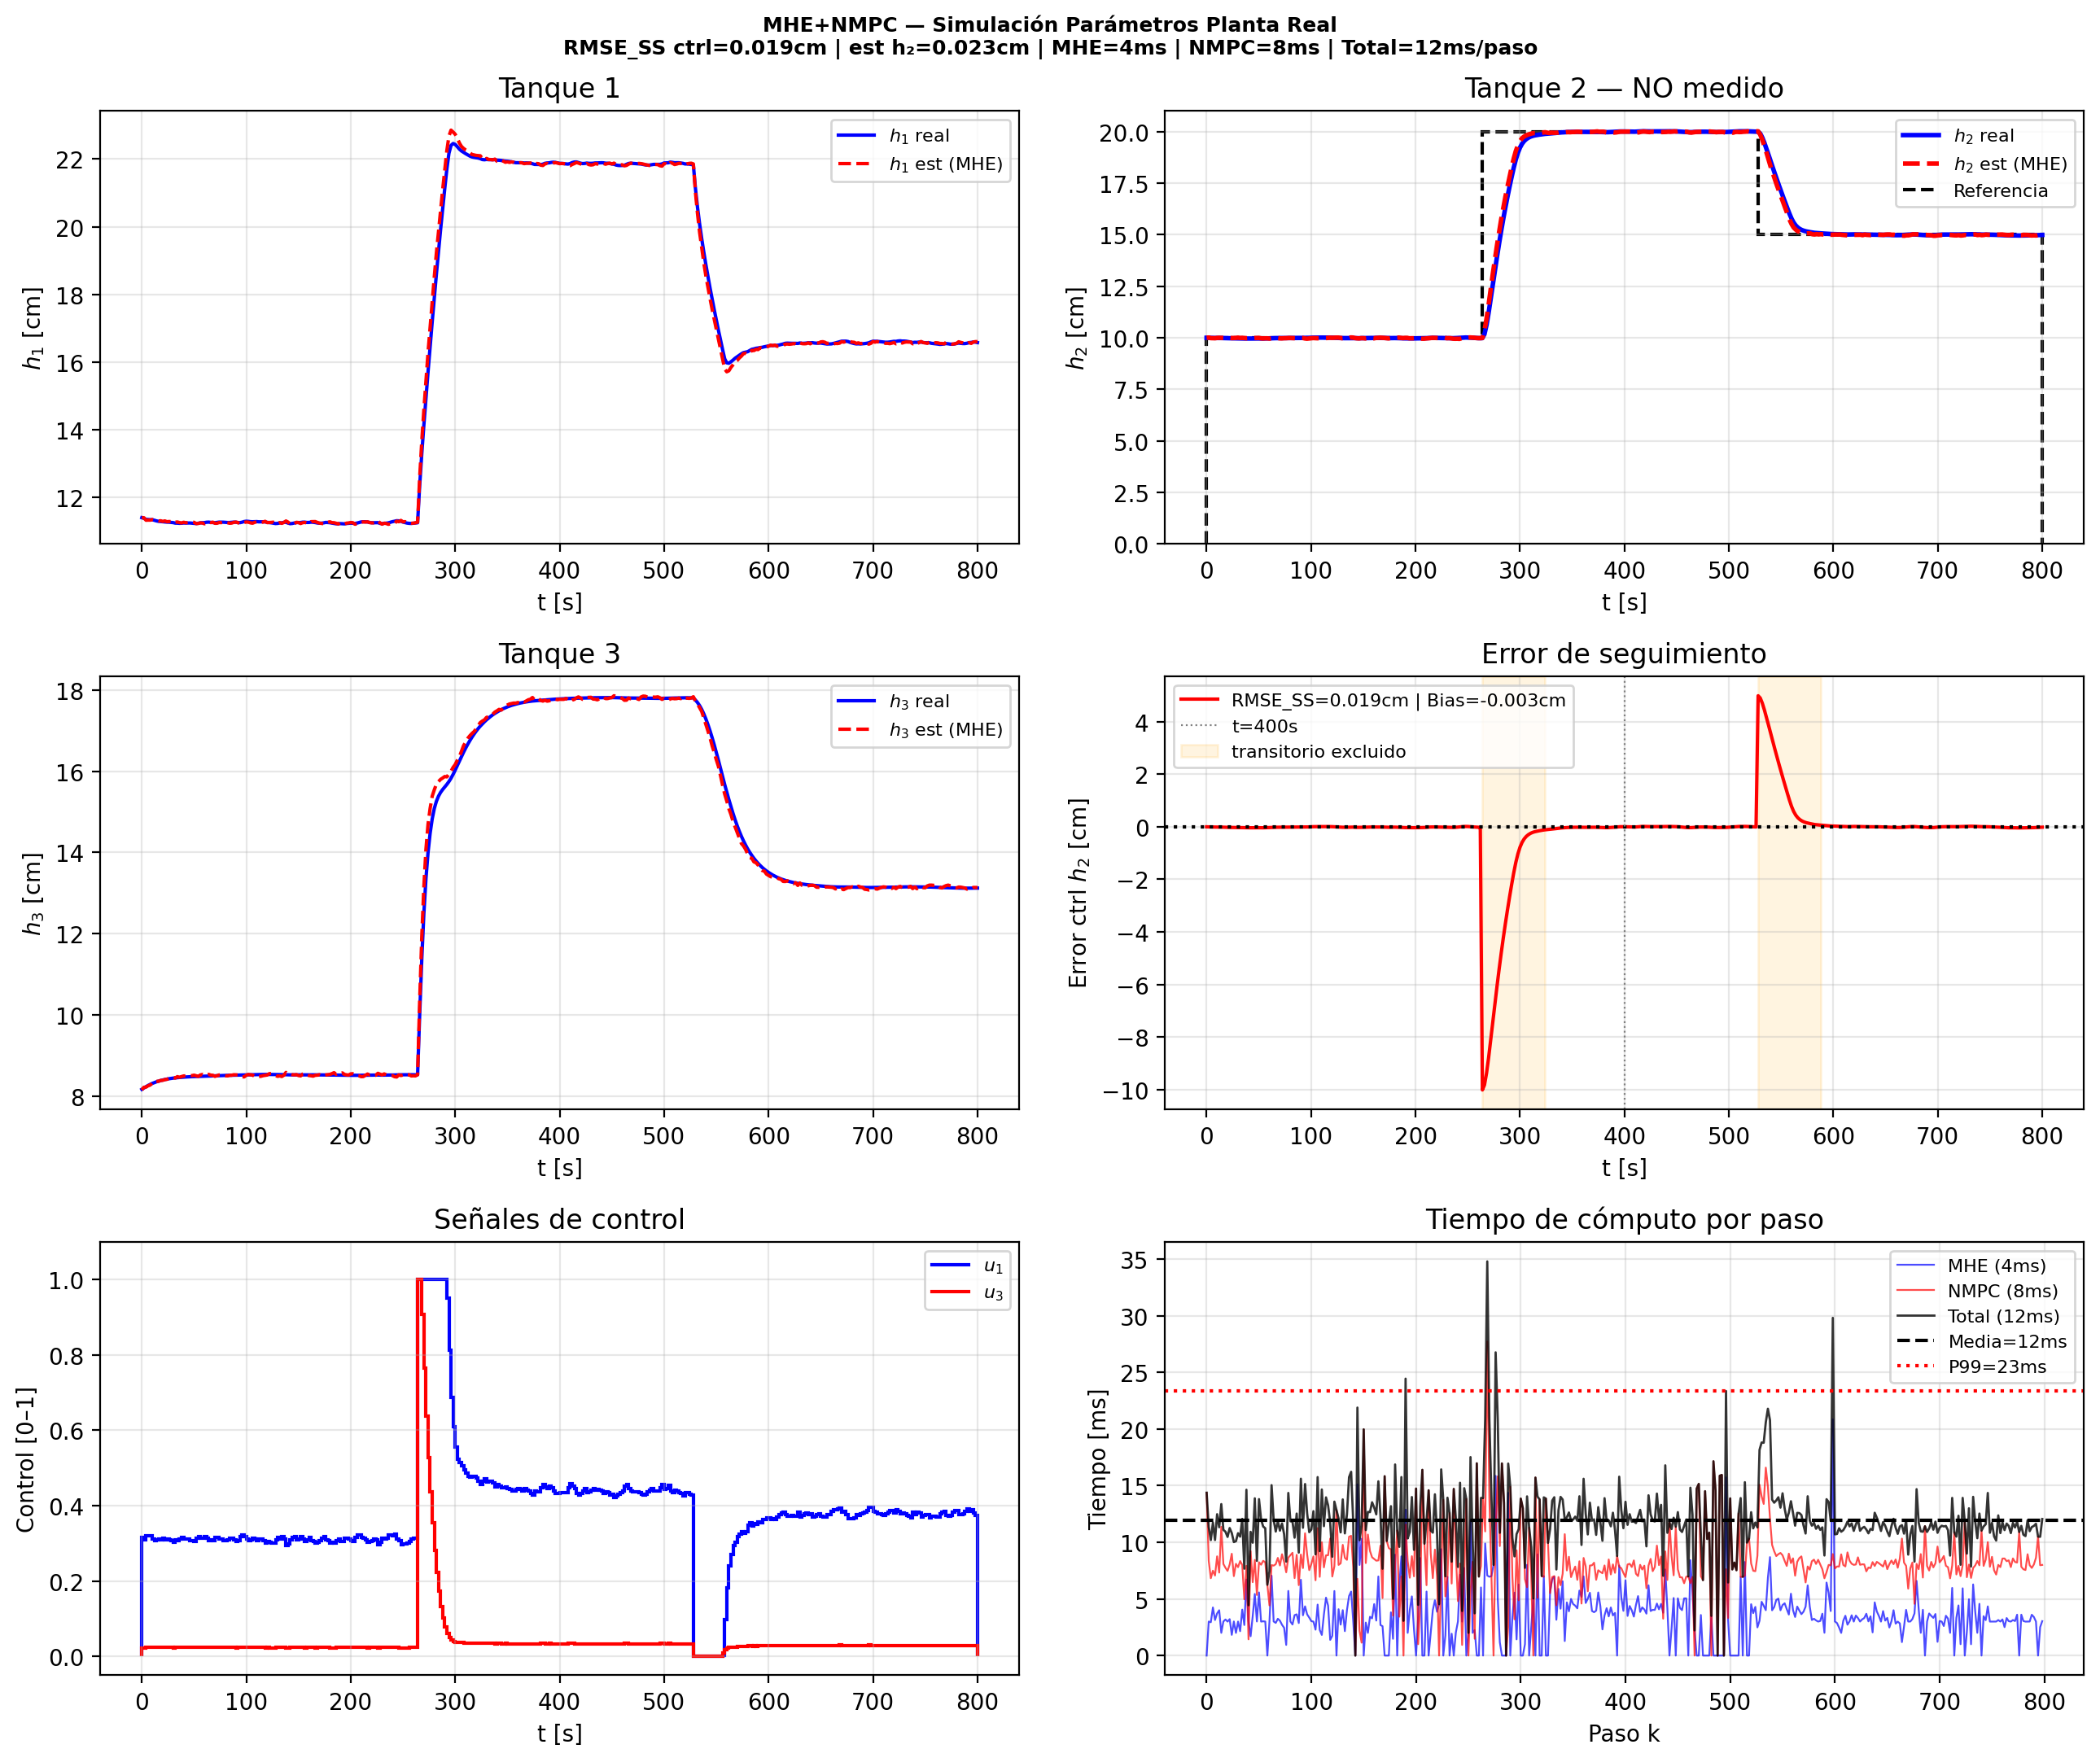
\includegraphics[width=\textwidth]{img/mhe_nmpc_closed_loop_planta_real.png}
    \caption{Lazo cerrado MHE+NMPC en simulación
    ($\sigma = 1$~mm). $\mathrm{RMSE}_{\mathrm{SS}} = 0.019$~cm,
    sesgo $= -0.003$~cm, tiempo medio $= 13$~ms/paso. El transitorio
    al cambio de referencia~0.10$\to$0.20~m sin suavización
    produce un subimpulso de $\approx -10$~cm que se excluye de
    la métrica $\mathrm{RMSE}_{\mathrm{SS}}$.}
    \label{fig:mhe_nmpc_sim}
\end{figure}

\begin{figure}[H]
    \centering
    \includegraphics[width=\textwidth]{img/koopman_v4_sim_planta_real.png}
    \caption{Lazo cerrado esquema Koopman en simulación 
    ($\sigma = 1$~mm, $k_i = 50$, \textit{deadband} $= 3$~cm). 
    $\mathrm{RMSE}_{\mathrm{SS}} = 0.026$~cm,
    sesgo $\approx 0$~cm, tiempo medio $= 8.4$~ms/paso.}
    \label{fig:koop_lc_sim}
\end{figure}
\begin{table}[H]
\centering
\caption{Comparación en lazo cerrado (simulación,
$T_s = 2$~s, $\sigma = 1$~mm, $N = 20$, $q = 500$).}
\label{tab:cmp_cl_sim}
\resizebox{\textwidth}{!}{%
\begin{tabular}{lccc}
\toprule
\textbf{Métrica} & \textbf{MHE+NMPC} & \textbf{Koopman} &
\textbf{Diferencia} \\
\midrule
$\mathrm{RMSE}_{\mathrm{SS}}$ [cm] & 0.019 & 0.026 &
$+27\%$ (MHE+NMPC mejor) \\
Sesgo en estado estacionario [cm]  & $-0.003$ & $\approx 0$ &
Ambos sin sesgo apreciable \\
Transitorio 0.10$\to$0.20~m       & subimpulso $\approx-10$~cm &
suave (rampa)           & Koopman con suavización \\
Tiempo medio por paso [ms]         & 13 & 8.4 &
$1.5\times$ más rápido \\
Tiempo p99 por paso [ms]           & 22 & 12.2 &
$1.8\times$ más rápido \\
\bottomrule
\end{tabular}}
\end{table}

Las Figuras~\ref{fig:mhe_nmpc_sim} y~\ref{fig:koop_lc_sim}
muestran las trayectorias de seguimiento de $h_2$ para ambos
esquemas. La Tabla~\ref{tab:cmp_cl_sim} cuantifica la
comparación en régimen permanente: el MHE+NMPC alcanza
$\mathrm{RMSE}_{\mathrm{SS}} = 0.019$~cm frente a $0.026$~cm
del esquema Koopman, siendo un $27\%$ mejor en estado
estacionario cuando el modelo coincide exactamente con la planta.
Ambos esquemas presentan sesgo prácticamente nulo.

Sin embargo, los comportamientos transitorios difieren
cualitativamente. El esquema Koopman incorpora un prefiltro
de referencia en rampa, una técnica estándar de conformación
de trayectoria en control predictivo, que suaviza los escalones
y elimina el sobreimpulso transitorio observado en versiones
previas del esquema al recibir un escalón completo de $10$~cm.
Para evaluar si esta misma estrategia de suavización podría
beneficiar también al benchmark, el prefiltro de rampa se probó
adicionalmente sobre el MHE+NMPC en un experimento independiente
sobre la planta física (no en el modelo de simulación de esta
subsección). Partiendo del desempeño experimental de referencia
reportado en la Sección~\ref{sec:resultados_exp}
($\mathrm{RMSE}_{\mathrm{SS}} = 0.354$~cm, sesgo $= -0.317$~cm,
Tabla~\ref{tab:cmp_exp}), la incorporación de la rampa degradó el
desempeño del benchmark ($\mathrm{RMSE}_{\mathrm{SS}}$ pasó a
$0.479$~cm, sesgo a $-0.443$~cm). En consecuencia, el benchmark se
mantiene sin prefiltro tanto en simulación como en planta física,
configuración en la que logra su desempeño óptimo en ambos
entornos. Esta asimetría no invalida la comparación:
independientemente de que el MHE+NMPC opere con o sin prefiltro
de rampa, el esquema Koopman lo supera en $\mathrm{RMSE}_{\mathrm{SS}}$.
La ventaja computacional del esquema Koopman es moderada:
$8.4$~ms frente a $13$~ms en tiempo medio ($1.5\times$) y
$12.2$~ms frente a $22$~ms en el percentil~99 ($1.8\times$).

Estos resultados en simulación revelan un patrón que los
experimentos físicos invierten: cuando modelo y planta
coinciden, el MHE+NMPC supera al esquema Koopman en
$\mathrm{RMSE}_{\mathrm{SS}}$; cuando aparecen las
discrepancias modelo--planta inevitables en la planta real,
la situación se revierte. La pregunta central que responden
los experimentos físicos es cuánto degrada cada esquema al
abandonar las condiciones ideales de simulación.
%% ================================================================
\subsection{Resultados Experimentales en Planta Física}
\label{sec:resultados_exp}
%% ================================================================

La validación experimental se llevó a cabo sobre la planta 
física descrita en la Sección~\ref{sec:planta_fisica}, 
siguiendo el protocolo de cinco corridas independientes por 
método establecido en la Sección~\ref{sec:validacion}. Se 
comparan el esquema Koopman y el benchmark MHE+NMPC, ambos 
operando en lazo cerrado sobre la misma planta y bajo la 
misma secuencia de referencias. Todas las métricas se 
calcularon sobre el régimen permanente definido como 
$t > 400$~s excluyendo los $60$~s posteriores a cada cambio 
de referencia, sobre un total de $400$ muestras por corrida.

\subsubsection{Métricas globales de régimen permanente}
\label{sec:metricas_globales}

La Tabla~\ref{tab:cmp_exp} consolida las métricas de las 
diez corridas experimentales, incluyendo el 
$\mathrm{RMSE}_{\mathrm{SS}}$, el RMSE transitorio, el MAE, 
el sesgo, la desviación estándar del error y el error máximo 
instantáneo en régimen permanente.

\begin{table}[H]
\centering
\caption{Resultados experimentales completos: esquema Koopman 
frente a MHE+NMPC sobre la planta física (cinco corridas por 
método, $400$ muestras por corrida). Todas las métricas en cm. 
$\mathrm{RMSE}_{\mathrm{tr}}$: RMSE incluyendo transitorios 
($t > 400$~s sin exclusión de ventanas de asentamiento).}
\label{tab:cmp_exp}
\resizebox{\textwidth}{!}{%
\begin{tabular}{llccccccc}
\toprule
\textbf{Método} & \textbf{Corrida} & 
$\mathbf{RMSE_{SS}}$ & $\mathbf{RMSE_{tr}}$ & 
\textbf{MAE} & \textbf{Bias} & 
$\boldsymbol{\sigma_{\mathrm{err}}}$ & \textbf{Err. máx.} \\
\midrule
Koopman 
  & Run 1 & 0.204 & 2.656 & 0.174 & $-$0.009 & 0.204 & 0.423 \\
  & Run 2 & 0.202 & 2.732 & 0.168 & $-$0.002 & 0.203 & 0.501 \\
  & Run 3 & 0.224 & 2.746 & 0.189 & $-$0.003 & 0.225 & 0.463 \\
  & Run 4 & 0.187 & 2.691 & 0.156 & $-$0.013 & 0.188 & 0.425 \\
  & Run 5 & 0.183 & 2.651 & 0.152 & $-$0.012 & 0.183 & 0.441 \\
\midrule
MHE+NMPC
  & Run 1 & 0.405 & 2.026 & 0.361 & $-$0.361 & 0.183 & 0.981 \\
  & Run 2 & 0.321 & 2.158 & 0.285 & $-$0.285 & 0.148 & 0.637 \\
  & Run 3 & 0.340 & 2.192 & 0.311 & $-$0.311 & 0.136 & 0.664 \\
  & Run 4 & 0.388 & 2.067 & 0.344 & $-$0.344 & 0.180 & 0.853 \\
  & Run 5 & 0.314 & 2.150 & 0.283 & $-$0.283 & 0.136 & 0.716 \\
\midrule
\multicolumn{2}{l}{\textbf{Koopman (media $\pm\sigma$)}} & 
  $\mathbf{0.200\pm0.016}$ & $2.695\pm0.040$ & 
  $0.168\pm0.015$ & $-0.008\pm0.005$ & 
  $0.200\pm0.016$ & $0.451\pm0.034$ \\
\multicolumn{2}{l}{\textbf{MHE+NMPC (media $\pm\sigma$)}} & 
  $0.354\pm0.041$ & $2.119\pm0.067$ & 
  $0.317\pm0.037$ & $-0.317\pm0.037$ & 
  $0.157\pm0.024$ & $0.770\pm0.146$ \\
\bottomrule
\end{tabular}}
\end{table}

Los resultados de la Tabla~\ref{tab:cmp_exp} revelan un 
cuadro de desempeño con ventajas diferenciadas según la fase 
del experimento. En régimen permanente, el esquema Koopman 
supera al MHE+NMPC en todas las métricas de precisión: el 
$\mathrm{RMSE}_{\mathrm{SS}}$ medio es $0.200$~cm frente a 
$0.354$~cm, una reducción del $43.4\%$, con rangos que no 
se solapan ($[0.183, 0.224]$~cm frente a $[0.314, 0.405]$~cm), 
lo que confirma que la diferencia es sistemática y no 
atribuible a variabilidad entre corridas. El sesgo en estado 
estacionario es la métrica más reveladora: el esquema Koopman
mantiene un bias medio de $-0.008$~cm con dispersión de
$\pm 0.005$~cm entre corridas, mientras que el MHE+NMPC
presenta un bias negativo sistemático de $-0.317$~cm con
dispersión de $\pm 0.037$~cm. Esto representa un contraste de
cerca de dos órdenes de magnitud en valor absoluto y de un factor
superior a $7$ en estabilidad entre corridas. La situación se invierte
en el régimen transitorio: el $\mathrm{RMSE}_{\mathrm{tr}}$ 
del MHE+NMPC es $2.119$~cm frente a $2.695$~cm del esquema 
Koopman, una diferencia del $21.4\%$ a favor del benchmark, 
debida a su ventana de memoria de $20$ pasos que le permite 
acumular evidencia sobre $h_2$ antes de que el controlador 
tome decisiones. En cuanto a la dispersión intra-muestra del 
error, $\sigma_{\mathrm{err}}$ es mayor para el esquema
Koopman ($0.200$~cm frente a $0.157$~cm), consecuencia de la
acción correctiva más frecuente del integrador. Sin embargo,
el error máximo instantáneo es sustancialmente menor para
Koopman ($0.451$~cm frente a $0.770$~cm), lo que indica que,
a pesar de su mayor varianza relativa, el esquema Koopman no
produce excursiones grandes del error como las que sí
presenta el MHE+NMPC en algunas corridas (Run~1, error
máximo de $0.981$~cm).

\subsubsection{Comparación directa de estimación de $h_2$}
\label{sec:est_h2_exp}

La planta dispone de un sensor de nivel en el tanque~2 cuyas
mediciones, no utilizadas en el lazo de control, permiten
cuantificar directamente el error de estimación
$h_2^{\mathrm{real}} - \hat{h}_2$ para ambos esquemas.
La Tabla~\ref{tab:cmp_est_h2} presenta esta comparación
sobre las diez corridas experimentales, en régimen permanente
($t > 400$~s, excluyendo ventanas de $60$~s post-cambio).

\begin{table}[H]
\centering
\caption{Comparación directa de estimación de $h_2$ frente
a verdad-terreno (sensor físico en tanque~2). $\mathrm{RMSE}_{\mathrm{est}}$:
error cuadrático medio de $h_2^{\mathrm{real}}-\hat{h}_2$ en
régimen permanente. $\mathrm{Bias}_{\mathrm{est}}$: valor
medio del mismo error (positivo = subestimación de $h_2$).
Todas las métricas en cm.}
\label{tab:cmp_est_h2}
\resizebox{\textwidth}{!}{%
\begin{tabular}{llcc}
\toprule
\textbf{Método} & \textbf{Corrida} &
$\mathbf{RMSE_{est}}$ & $\mathbf{Bias_{est}}$ \\
\midrule
Koopman
  & Run 1 & 0.688 & $+$0.411 \\
  & Run 2 & 0.691 & $+$0.397 \\
  & Run 3 & 0.675 & $+$0.411 \\
  & Run 4 & 0.678 & $+$0.462 \\
  & Run 5 & 0.705 & $+$0.438 \\
\midrule
MHE+NMPC
  & Run 1 & 0.578 & $+$0.234 \\
  & Run 2 & 0.608 & $+$0.255 \\
  & Run 3 & 0.542 & $+$0.183 \\
  & Run 4 & 0.563 & $+$0.194 \\
  & Run 5 & 0.579 & $+$0.202 \\
\midrule
\multicolumn{2}{l}{\textbf{Koopman (media $\pm\sigma$)}} &
  $0.687\pm0.011$ & $+0.424\pm0.023$ \\
\multicolumn{2}{l}{\textbf{MHE+NMPC (media $\pm\sigma$)}} &
  $\mathbf{0.574\pm0.022}$ & $+0.214\pm0.027$ \\
\bottomrule
\end{tabular}}
\end{table}

Los resultados de la Tabla~\ref{tab:cmp_est_h2} revelan que
el MHE+NMPC estima $h_2$ con mayor precisión que el
observador de Koopman: $\mathrm{RMSE}_{\mathrm{est}} =
0.574\pm0.022$~cm frente a $0.687\pm0.011$~cm, una mejora
del $16.5\%$. Ambos estimadores presentan un sesgo positivo
sistemático, es decir, subestiman $h_2$, pero el del MHE+NMPC
($+0.214$~cm) es casi la mitad del del observador de
Koopman ($+0.424$~cm). Esta diferencia es físicamente
coherente con la ventaja estructural del MHE: su ventana de
$N = 20$ pasos de memoria acumula evidencia sobre la
evolución de $h_2$ antes de emitir una estimación, mientras
que el observador de Luenberger corrige en un único paso con
una ganancia pequeña impuesta por la DARE.

La interpretación conjunta con la Tabla~\ref{tab:cmp_exp} es
central para entender los resultados del trabajo: el MHE
estima $h_2$ más precisamente, pero ese beneficio se
transfiere a la acción de control con un sesgo residual de
$-0.317$~cm que el NMPC no puede compensar por sí solo. El
observador de Koopman, aunque menos preciso
($\mathrm{RMSE}_{\mathrm{est}}$ un $16.5\%$ mayor), opera
junto con un integrador que acumula el error de seguimiento
de $\hat{h}_2$ respecto a la referencia y fuerza una
corrección activa, eliminando el sesgo en control hasta
$-0.008$~cm. El esquema Koopman sacrifica precisión de
estimación instantánea para ganar robustez de seguimiento
en régimen permanente mediante la acción integral.

\subsubsection{Esfuerzo de control}
\label{sec:esfuerzo}

\begin{table}[H]
\centering
\caption{Esfuerzo de control comparado (valores medios de 
las cinco corridas experimentales). TV: variación total de 
la señal de control sobre los $400$ pasos del experimento; 
$\bar{u}$: valor medio de la señal de control.}
\label{tab:ctrl_effort}
\begin{tabular}{lcccc}
\toprule
\textbf{Método} & \textbf{TV $u_1$} & \textbf{TV $u_3$} & 
\textbf{$\bar{u}_1$} & \textbf{$\bar{u}_3$} \\
\midrule
Koopman  & 53.31 & 4.51 & 0.364 & 0.032 \\
MHE+NMPC & 14.70 & 2.98 & 0.456 & 0.050 \\
\bottomrule
\end{tabular}
\end{table}

El esfuerzo de control del esquema Koopman es $3.6$ veces 
mayor en variación total de $u_1$ ($53.31$ frente a $14.70$) 
y $1.5$ veces mayor en $u_3$ ($4.51$ frente a $2.98$). Sin 
embargo, los valores medios de control son menores para el 
esquema Koopman ($\bar{u}_1 = 0.364$ frente a $0.456$; 
$\bar{u}_3 = 0.032$ frente a $0.050$), lo que indica que el 
mayor esfuerzo de control no se traduce en mayor consumo 
energético neto sino en una regulación más activa alrededor 
de la referencia, coherente con la acción integradora del 
KoopmanMPC.

\subsubsection{Comparación visual de las trayectorias}
\label{sec:overlay}

\begin{figure}[H]
    \centering
    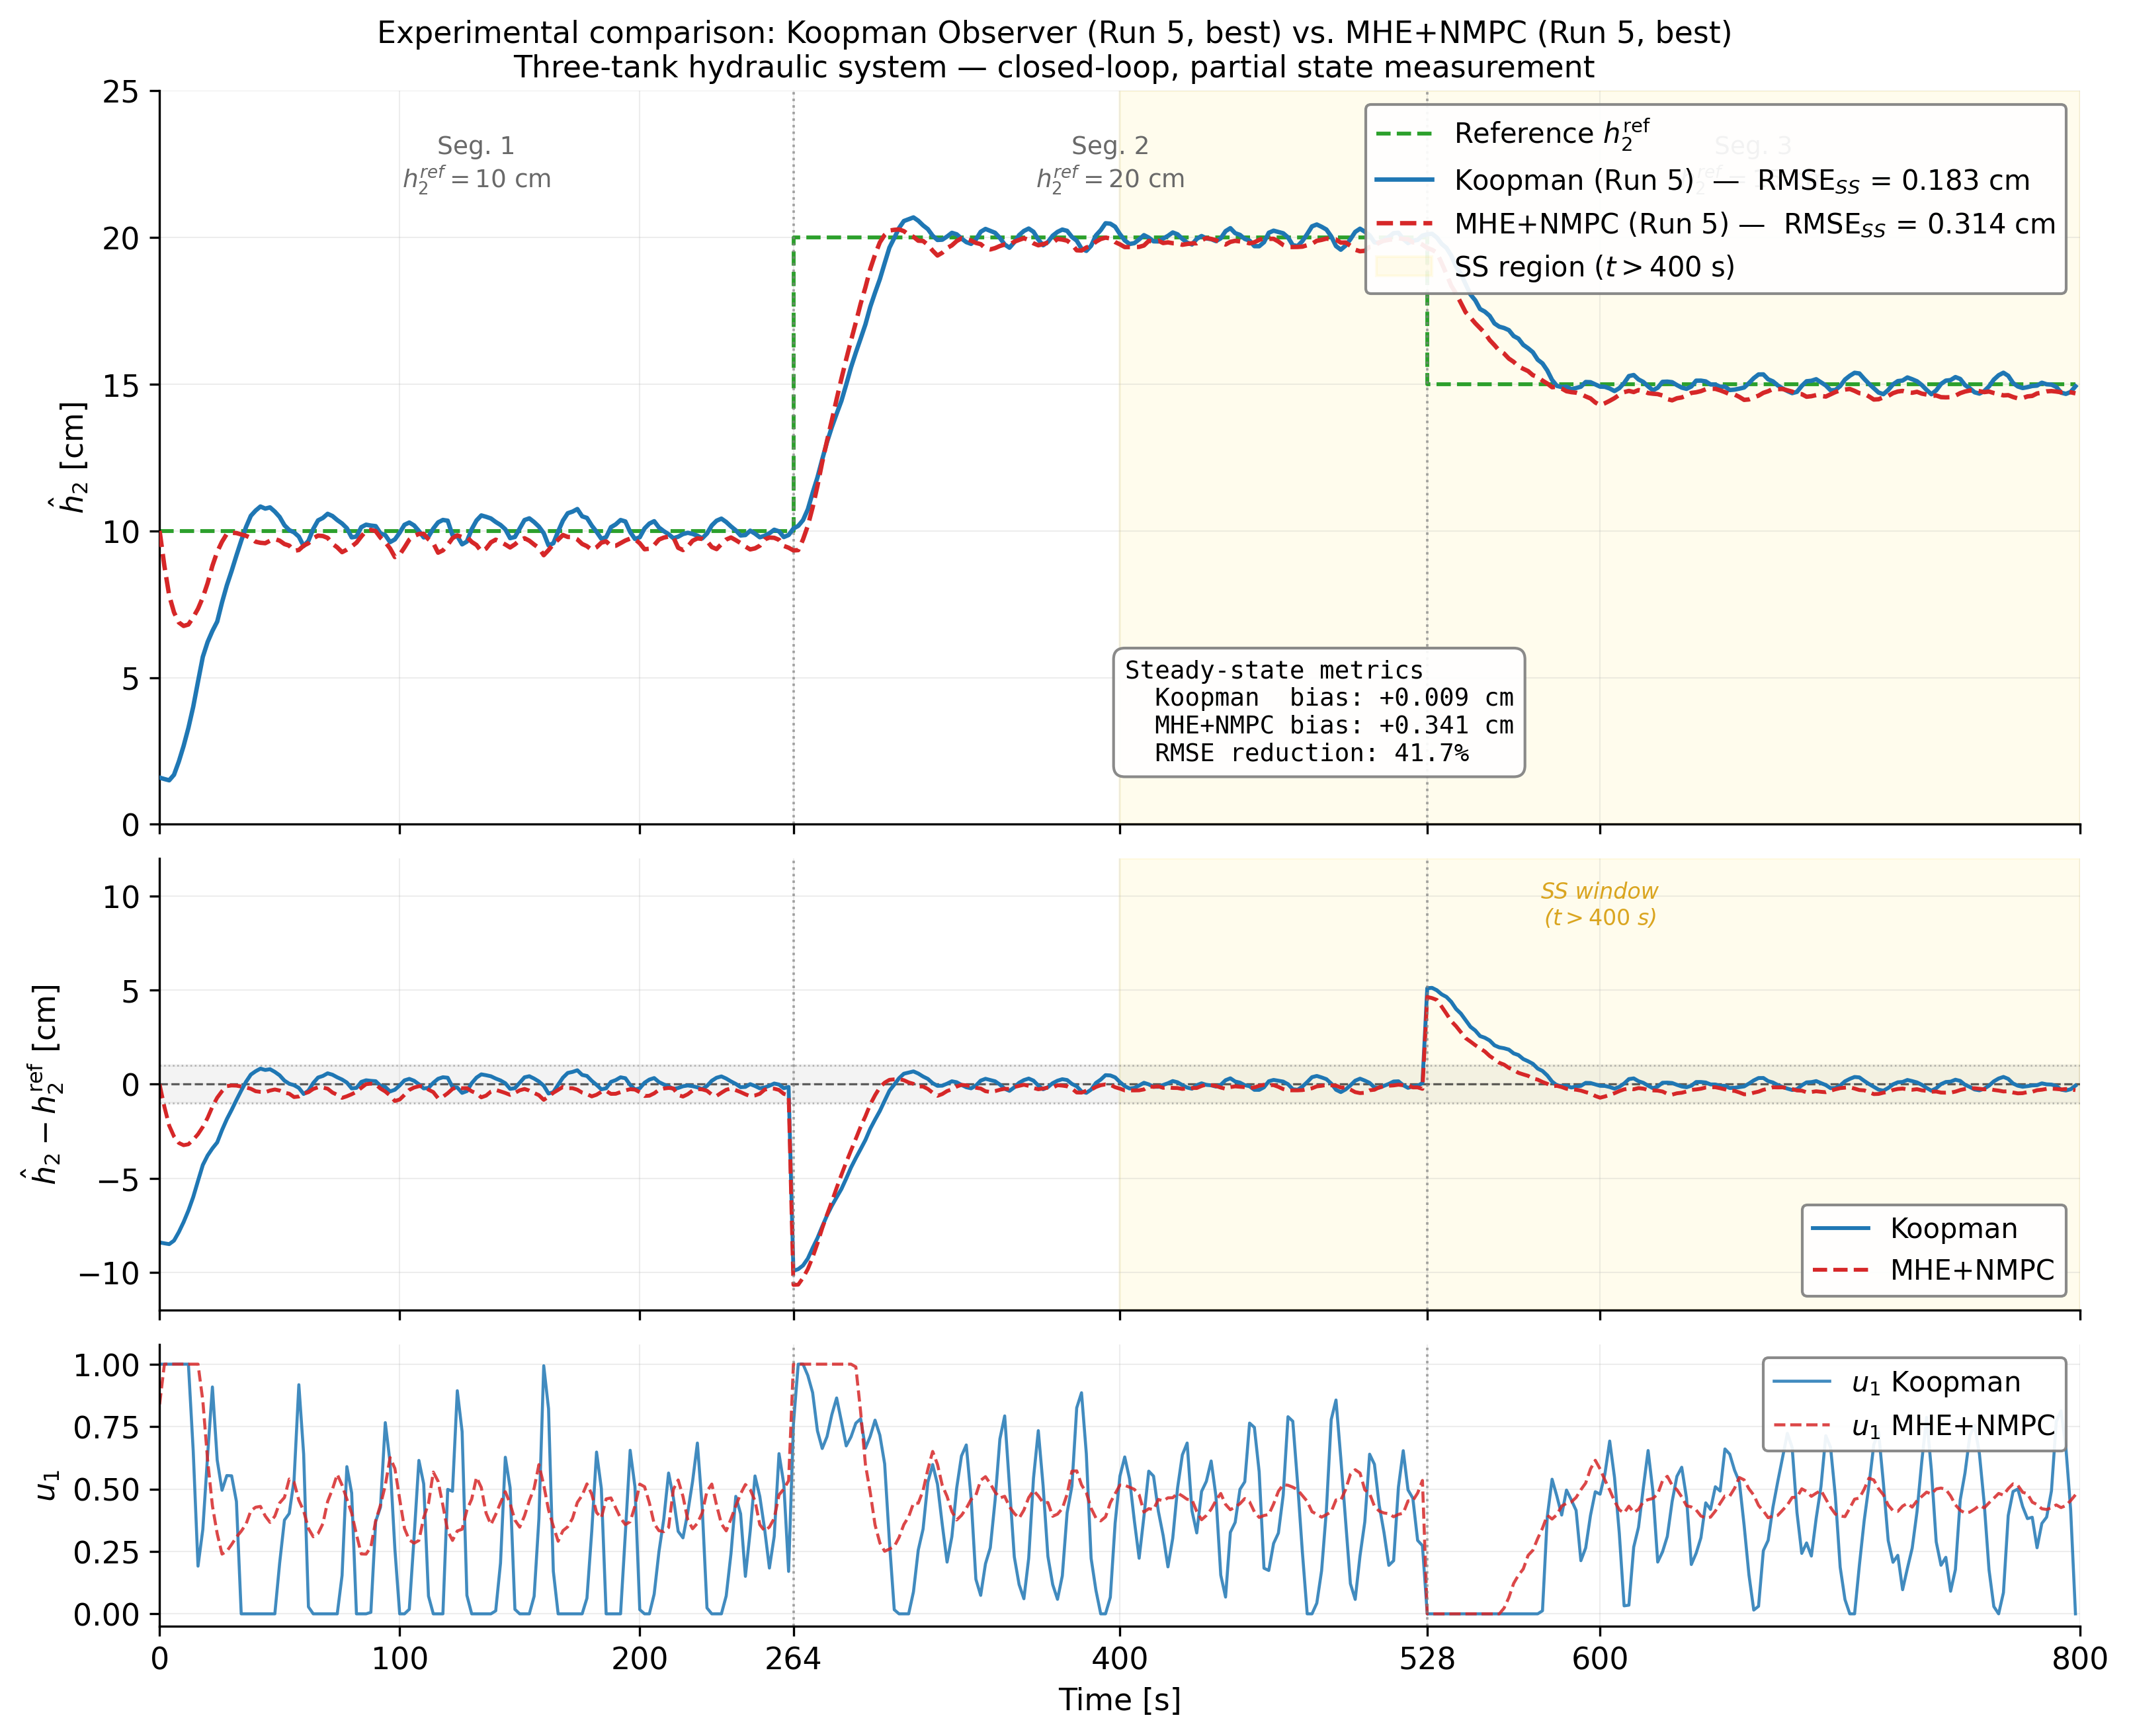
\includegraphics[width=\textwidth]{img/overlay_experimental.png}
    \caption{Comparación experimental entre la mejor corrida 
    del esquema Koopman (Run~5, 
    $\mathrm{RMSE}_{\mathrm{SS}} = 0.183$~cm, línea continua 
    azul) y la mejor corrida del MHE+NMPC (Run~5, 
    $\mathrm{RMSE}_{\mathrm{SS}} = 0.314$~cm, línea 
    discontinua roja). Panel superior: nivel estimado de 
    $h_2$ y referencia escalonada (línea verde discontinua). 
    Panel central: error de seguimiento 
    $\hat{h}_2 - h_2^{\mathrm{ref}}$ en cm. Panel inferior: 
    señal de control $u_1$. Las líneas verticales punteadas 
    marcan los cambios de referencia en $t = 264$~s y 
    $t = 528$~s; la región sombreada en dorado corresponde 
    a la ventana de cómputo del régimen permanente 
    ($t > 400$~s).}
    \label{fig:overlay_exp}
\end{figure}

La Figura~\ref{fig:overlay_exp} superpone la mejor corrida 
de cada método para facilitar la comparación visual directa. 
En el panel superior se observa que el esquema Koopman sigue 
la referencia con mayor proximidad en los tres tramos de 
régimen permanente. El panel central evidencia que el error 
del esquema Koopman oscila simétricamente en torno a cero 
con amplitud inferior a $\pm 0.3$~cm durante el régimen 
permanente, mientras que el error del MHE+NMPC se desplaza 
sistemáticamente hacia valores negativos. En el panel 
inferior, las señales de control son cualitativamente 
similares en magnitud media, pero la mayor variación total 
del esquema Koopman se manifiesta como ajustes más frecuentes 
de $u_1$ alrededor de su valor de régimen permanente.

\subsubsection{Desglose por segmentos de referencia}
\label{sec:segmentos}

Las Tablas~\ref{tab:seg_rmse} y~\ref{tab:seg_bias} desglosan 
el $\mathrm{RMSE}_{\mathrm{SS}}$ y el sesgo por tramo de 
referencia y por corrida, permitiendo determinar si la 
ventaja del esquema Koopman es uniforme en todo el rango 
de operación o se concentra en niveles específicos.

\begin{table}[H]
\centering
\caption{$\mathrm{RMSE}_{\mathrm{SS}}$ por segmento de 
referencia y por corrida (régimen permanente tras excluir 
los primeros $60$~s de cada tramo). Valores en cm.}
\label{tab:seg_rmse}
\footnotesize
\setlength{\tabcolsep}{4pt}
\begin{tabular}{llccc}
\toprule
\textbf{Método} & \textbf{Corrida} & 
\textbf{Seg.~1 ($0.10$~m)} & 
\textbf{Seg.~2 ($0.20$~m)} & 
\textbf{Seg.~3 ($0.15$~m)} \\
\midrule
Koopman 
  & Run 1 & 0.206 & 0.228 & 0.187 \\
  & Run 2 & 0.232 & 0.215 & 0.199 \\
  & Run 3 & 0.240 & 0.220 & 0.215 \\
  & Run 4 & 0.228 & 0.233 & 0.154 \\
  & Run 5 & 0.288 & 0.206 & 0.180 \\
  & \textbf{Media} & \textbf{0.239} & \textbf{0.220} & 
    \textbf{0.187} \\
\midrule
MHE+NMPC
  & Run 1 & 0.514 & 0.304 & 0.444 \\
  & Run 2 & 0.450 & 0.241 & 0.358 \\
  & Run 3 & 0.470 & 0.293 & 0.368 \\
  & Run 4 & 0.447 & 0.292 & 0.432 \\
  & Run 5 & 0.445 & 0.234 & 0.360 \\
  & \textbf{Media} & \textbf{0.465} & \textbf{0.273} & 
    \textbf{0.392} \\
\midrule
\multicolumn{2}{l}{\textbf{Mejora Koopman vs. MHE+NMPC}} & 
  $\mathbf{48.6\%}$ & $\mathbf{19.4\%}$ & $\mathbf{52.3\%}$ \\
\bottomrule
\end{tabular}
\end{table}

\begin{table}[H]
\centering
\caption{Sesgo (bias) en estado estacionario por segmento 
de referencia y por corrida. Valores en cm. Un valor 
negativo indica que la estimación subestima 
sistemáticamente el nivel real.}
\label{tab:seg_bias}
\footnotesize
\setlength{\tabcolsep}{4pt}
\begin{tabular}{llccc}
\toprule
\textbf{Método} & \textbf{Corrida} & 
\textbf{Bias Seg.~1 ($0.10$~m)} & 
\textbf{Bias Seg.~2 ($0.20$~m)} & 
\textbf{Bias Seg.~3 ($0.15$~m)} \\
\midrule
Koopman 
  & Run 1 & 0.016 & $-$0.002 & $-$0.010 \\
  & Run 2 & 0.041 & 0.010 & $-$0.005 \\
  & Run 3 & 0.040 & $-$0.005 & $-$0.004 \\
  & Run 4 & 0.023 & $-$0.006 & $-$0.020 \\
  & Run 5 & 0.065 & 0.008 & $-$0.014 \\
  & \textbf{Media} & \textbf{0.037} & \textbf{0.001} & 
    $-$\textbf{0.011} \\
\midrule
MHE+NMPC
  & Run 1 & $-$0.478 & $-$0.265 & $-$0.406 \\
  & Run 2 & $-$0.416 & $-$0.196 & $-$0.334 \\
  & Run 3 & $-$0.442 & $-$0.244 & $-$0.350 \\
  & Run 4 & $-$0.414 & $-$0.232 & $-$0.403 \\
  & Run 5 & $-$0.404 & $-$0.197 & $-$0.341 \\
  & \textbf{Media} & $-$\textbf{0.431} & $-$\textbf{0.227} & 
    $-$\textbf{0.367} \\
\bottomrule
\end{tabular}
\end{table}

El análisis por segmentos de la Tabla~\ref{tab:seg_rmse} 
revela que la ventaja del esquema Koopman es consistente 
en los tres niveles de referencia pero con una variación 
sistemática y físicamente coherente. En los segmentos
extremos, $0.10$~m y $0.15$~m, la mejora en
$\mathrm{RMSE}_{\mathrm{SS}}$ es del $48.6\%$ y $52.3\%$
respectivamente, mientras que en el segmento central de 
$0.20$~m la mejora se reduce al $19.4\%$. La razón física 
de este patrón reside en la curvatura de la no linealidad 
de Torricelli: a niveles bajos, la derivada 
$d^2\sqrt{h}/dh^2 = -1/(4h^{3/2})$ es más pronunciada, 
lo que hace que las linealizaciones locales en las que se 
apoya el MHE introduzcan un error de modelado mayor que 
el modelo EDMD global entrenado sobre todo el rango de 
operación. La Tabla~\ref{tab:seg_bias} confirma este 
mecanismo: el sesgo del esquema Koopman se mantiene en 
una banda estrecha en torno a cero en los tres segmentos 
(entre $-0.011$ y $0.037$~cm), mientras que el sesgo del 
MHE+NMPC muestra una dependencia fuerte del nivel de 
referencia, pasando de $-0.431$~cm en el segmento de 
$0.10$~m a $-0.227$~cm en el de $0.20$~m, coherente con 
la reducción de la curvatura de $\sqrt{h}$ al aumentar el 
nivel. Cabe notar que, a diferencia del MHE+NMPC, el sesgo 
del esquema Koopman cambia de signo entre segmentos 
(positivo en Seg.~1, prácticamente nulo en Seg.~2, 
ligeramente negativo en Seg.~3); esta oscilación de 
pequeña magnitud alrededor de cero es atribuible a la 
acción del \textit{deadband} del integrador, que tolera un 
remanente de error dentro de su banda de $\pm 3$~cm antes 
de corregirlo por completo, en contraste con el bias 
unidireccional y de mayor magnitud del MHE+NMPC.

\subsubsection{Análisis de repetibilidad}
\label{sec:repetibilidad}

\begin{figure}[H]
    \centering
    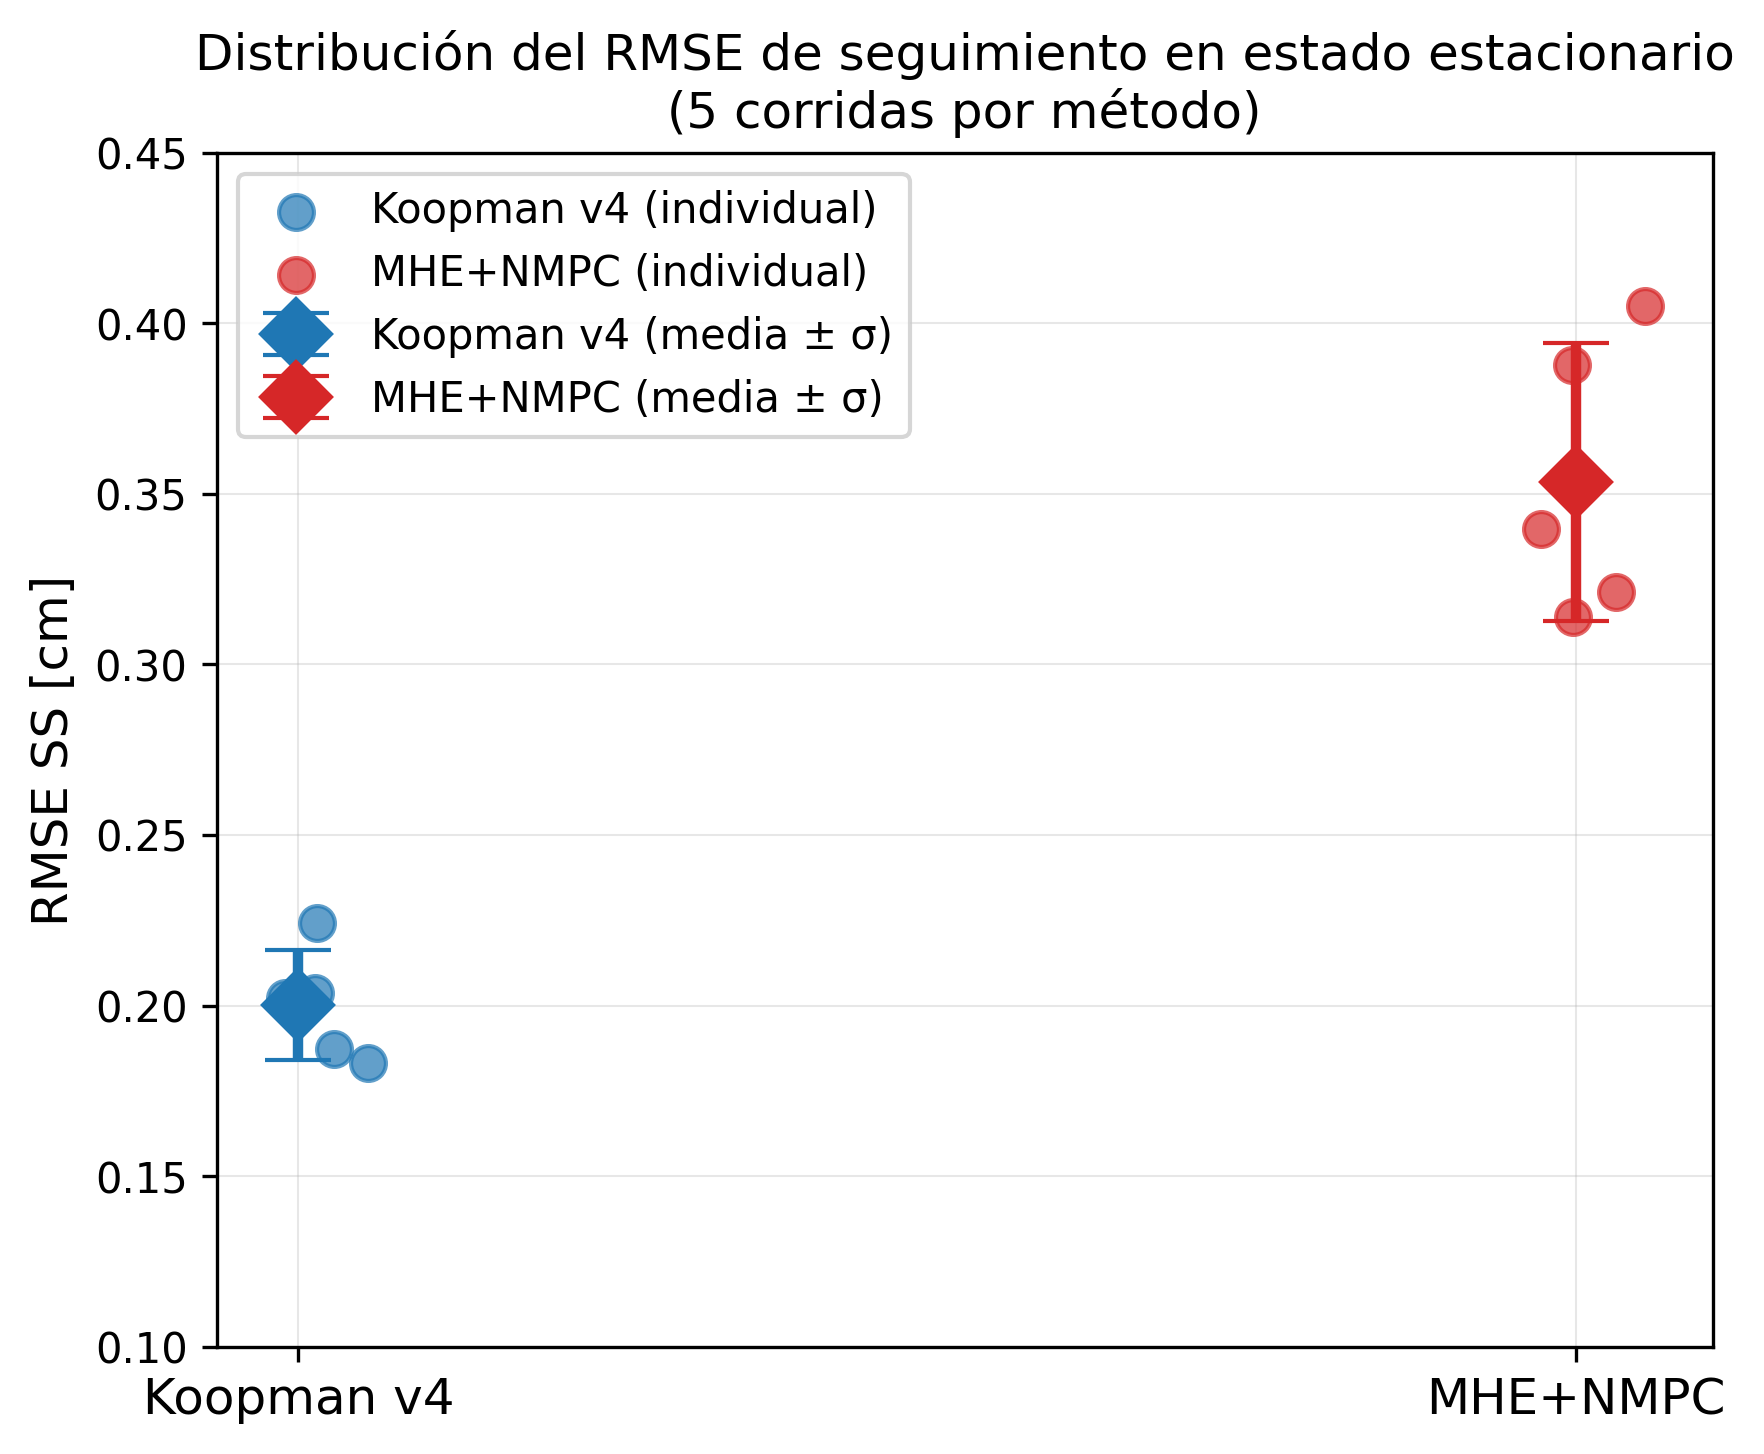
\includegraphics[width=\textwidth]{img/rmse_distribution.png}
    \caption{Distribución del $\mathrm{RMSE}_{\mathrm{SS}}$ 
    en las cinco corridas experimentales de cada método. Cada 
    punto representa una corrida individual; las líneas 
    horizontales indican el valor medio de cada método. Los 
    rangos de ambos métodos no se solapan: $[0.183, 0.224]$~cm 
    para el esquema Koopman y $[0.314, 0.405]$~cm para 
    MHE+NMPC, con una brecha mínima de $0.090$~cm entre la 
    peor corrida de Koopman y la mejor corrida del MHE+NMPC.}
    \label{fig:rmse_dist}
\end{figure}

La repetibilidad del desempeño se evalúa a través de la 
dispersión de las métricas entre las cinco corridas de cada 
método. La Figura~\ref{fig:rmse_dist} muestra la 
distribución del $\mathrm{RMSE}_{\mathrm{SS}}$ individual: 
la separación completa entre los dos conjuntos de valores, 
ahora confirmada sobre un total de diez corridas, refuerza la conclusión de que la ventaja del esquema 
Koopman es robusta a la variabilidad intrínseca de la planta 
entre corridas sucesivas. La desviación estándar del 
$\mathrm{RMSE}_{\mathrm{SS}}$ entre corridas es $0.016$~cm 
para el esquema Koopman y $0.041$~cm para el MHE+NMPC, lo 
que indica que, además de un RMSE medio menor, el esquema 
Koopman presenta una repetibilidad superior, con una 
dispersión relativa aproximadamente $2.6$ veces menor. La 
estabilidad del sesgo del esquema Koopman es particularmente 
notable: su desviación estándar entre corridas es 
$\pm 0.005$~cm, frente a $\pm 0.037$~cm del MHE+NMPC, una 
diferencia de un factor superior a $7$ que refleja que el 
integrador con \textit{deadband} converge a un sesgo cercano 
a nulo independientemente de las condiciones iniciales y de 
las pequeñas variaciones paramétricas entre corridas 
sucesivas.

\subsubsection{Análisis de la respuesta transitoria}
\label{sec:transitorios}

La Tabla~\ref{tab:transient} resume los tiempos de 
asentamiento al $\pm 5\%$ de la amplitud del escalón 
($T_s^{5\%}$) y el sobreimpulso máximo para cada segmento 
de referencia y cada corrida.

\begin{table}[H]
\centering
\caption{Tiempos de asentamiento al $\pm 5\%$ 
($T_s^{5\%}$, en segundos) y sobreimpulso máximo (OS, en 
cm) por segmento de referencia y por corrida.}
\label{tab:transient}
\footnotesize
\setlength{\tabcolsep}{3pt}
\begin{tabular}{llcccccc}
\toprule
\textbf{Método} & \textbf{Corrida} & 
\multicolumn{3}{c}{\textbf{$T_s^{5\%}$ [s]}} & 
\multicolumn{3}{c}{\textbf{OS [cm]}} \\
\cmidrule(lr){3-5}\cmidrule(lr){6-8}
& & Seg.~1 & Seg.~2 & Seg.~3 & 
  Seg.~1 & Seg.~2 & Seg.~3 \\
\midrule
Koopman 
  & Run 1 & 216 & 38 & 48 & 0.85 & 0.82 & 5.31 \\
  & Run 2 & 260 & 36 & 46 & 0.86 & 0.79 & 4.76 \\
  & Run 3 & 160 & 38 & 48 & 1.00 & 0.63 & 5.34 \\
  & Run 4 & 60  & 36 & 48 & 1.25 & 0.74 & 5.22 \\
  & Run 5 & 174 & 36 & 46 & 0.83 & 0.68 & 5.12 \\
  & \textbf{Media} & 174 & 37 & 47 & 0.96 & 0.73 & 5.15 \\
\midrule
MHE+NMPC
  & Run 1 & 262 & 28 & 90 & 0.09 & 0.48 & 4.92 \\
  & Run 2 & 262 & 30 & 34 & 0.00 & 0.46 & 4.65 \\
  & Run 3 & 254 & 34 & 36 & 0.00 & 0.41 & 4.62 \\
  & Run 4 & 262 & 30 & 78 & 0.00 & 0.34 & 4.44 \\
  & Run 5 & 262 & 32 & 36 & 0.03 & 0.27 & 4.64 \\
  & \textbf{Media} & \textbf{260} & \textbf{31} & 55 & 
    \textbf{0.02} & \textbf{0.39} & 4.65 \\
\bottomrule
\end{tabular}
\end{table}

El análisis transitorio revela un cuadro complementario 
al de régimen permanente. En el primer segmento 
($h_2^{\mathrm{ref}} = 0.10$~m), el esquema Koopman 
presenta un tiempo de asentamiento medio menor ($174$~s 
frente a $260$~s del MHE+NMPC), aunque con mayor 
variabilidad entre corridas (rango $[60, 260]$~s frente a 
$[254, 262]$~s del benchmark), y un sobreimpulso 
sustancialmente mayor ($0.96$~cm en media frente a 
$0.02$~cm). Este sobreimpulso es consecuencia de que el integrador puede 
acumular una pequeña carga durante el periodo inicial de 
acondicionamiento antes de que la \textit{deadband} lo 
congele. En el segundo segmento 
($h_2^{\mathrm{ref}} = 0.20$~m, transición ascendente 
de $+10$~cm), el MHE+NMPC muestra un tiempo de 
asentamiento sistemáticamente menor y de notable 
repetibilidad: entre $28$ y $34$~s en las cinco corridas, 
frente a $36$--$38$~s del esquema Koopman. En este
segmento la diferencia entre métodos es pequeña en 
términos absolutos ($6$--$9$~s). Esta diferencia refleja 
que el MHE, con su ventana de $20$ pasos de memoria 
temporal, proporciona una estimación del estado al inicio 
del nuevo segmento más informada que el observador de 
Luenberger de un solo paso. En el tercer segmento 
($h_2^{\mathrm{ref}} = 0.15$~m, transición descendente 
de $-5$~cm), el esquema Koopman mantiene tiempos de 
asentamiento consistentes entre corridas ($46$--$48$~s), 
mientras que el MHE+NMPC presenta una variabilidad 
considerablemente mayor ($34$ a $90$~s según la corrida, 
con media de $55$~s), de modo que en este segmento el 
esquema Koopman resulta en promedio más rápido y, sobre 
todo, más repetible. El sobreimpulso en el tercer segmento 
es similar en ambos métodos ($5.15$~cm para Koopman frente 
a $4.65$~cm para MHE+NMPC), confirmando que en las 
transiciones descendentes la dinámica dominante es el 
vaciado por gravedad y no la estrategia de control. La 
interpretación conjunta de los resultados transitorio y de 
régimen permanente muestra que la ventaja del MHE+NMPC en 
transitorio se concentra específicamente en el segmento de 
mayor amplitud de escalón ($+10$~cm), mientras que el 
esquema Koopman iguala o supera al benchmark en los
segmentos restantes. Además, lo supera de forma consistente en
régimen permanente gracias a la eliminación del sesgo por
el integrador.

\subsubsection{Presupuesto computacional}
\label{sec:computo}

\begin{table}[H]
\centering
\caption{Presupuesto computacional por paso para las diez 
corridas experimentales. Para el esquema Koopman el cuello 
de botella es el solver QP de CasADi; el observador de 
Luenberger contribuye menos de $1$~ms por ser una operación 
puramente algebraica. Para el MHE+NMPC, tanto el MHE como 
el NMPC resuelven programas no lineales con IPOPT. 
Tiempos en ms.}
\label{tab:timing_exp}
\begin{tabular}{llcc}
\toprule
\textbf{Método} & \textbf{Corrida} & 
\textbf{Media [ms]} & \textbf{P99 [ms]} \\
\midrule
Koopman
  & Run 1--5 (media) & $\approx$ 2\,100 & $\approx$ 2\,140 \\
\midrule
MHE+NMPC
  & Run 1--5 (media) & $\approx$ 2\,096 & $\approx$ 2\,543 \\
\bottomrule
\end{tabular}
\end{table}

En la implementación actual sobre la planta física, los 
tiempos totales medios de ambos métodos son similares 
($\approx 2\,100$~ms para Koopman frente a $\approx 2\,096$~ms 
para MHE+NMPC), enmascarados por la espera activa hasta 
completar el período de muestreo $T_s = 2$~s. La diferencia 
relevante aparece en el percentil $99$: el MHE+NMPC presenta 
picos ocasionales de hasta $2\,543$~ms, superando el período 
de muestreo, mientras que el esquema Koopman se mantiene 
acotado en $2\,140$~ms. Estos picos del MHE+NMPC son 
consistentes con la naturaleza no determinista de la 
convergencia de IPOPT en los dos NLPs (MHE y NMPC) que deben 
resolverse en cada paso, frente al QP convexo y de 
convergencia más predecible que resuelve el KoopmanMPC. Esta 
diferencia en la cola de la distribución del tiempo de 
cómputo es relevante para el despliegue embebido, donde una 
violación ocasional del período de muestreo puede 
comprometer la estabilidad del lazo cerrado si no se gestiona 
adecuadamente, como se hizo en este trabajo mediante el 
mecanismo de \textit{buffer} de última medición en el ESP32 
descrito en la Sección~\ref{sec:validacion}.


























\section{Análisis de Resultados}
\label{sec:analisis}

Los resultados presentados en la Sección~\ref{sec:resultados} 
permiten realizar una caracterización cuantitativa y física del 
desempeño relativo de los esquemas evaluados en tres niveles de 
complejidad progresiva: control puro con estado completo disponible, 
estimación pura en lazo abierto, y lazo cerrado completo tanto en 
simulación como en la planta física. Esta estructura permite 
desacoplar las contribuciones individuales del modelo de predicción 
y del estimador de estados al desempeño global del lazo, y 
proporciona una interpretación coherente de los resultados 
experimentales a la luz de los obtenidos en simulación.

%% ================================================================
\subsection{Control puro: NMPC frente a KoopmanMPC}
\label{sec:analisis_ctrl}
%% ================================================================

El primer experimento de simulación aisló el efecto del modelo de 
predicción al asumir acceso completo al vector de estado en cada 
instante de muestreo, eliminando así la contribución del estimador 
al error total del lazo. Bajo esta condición, el KoopmanMPC alcanzó 
un $\mathrm{RMSE}_{\mathrm{SS}}$ de $0.009$~cm frente a $0.015$~cm 
del NMPC, lo que representa una mejora del $40\%$ en precisión de 
seguimiento en estado estacionario. Incluso en el RMSE transitorio, 
que penaliza el comportamiento durante los cambios de referencia, el 
KoopmanMPC logra $\mathrm{RMSE}_{\mathrm{SS}} = 0.026$~cm en lazo
cerrado con estimador (comparable al MHE+NMPC en simulación ideal,
véase Sección~\ref{sec:lc_sim}), evidenciando que la representación
lineal global del espacio de Koopman captura la dinámica no lineal
del sistema con una fidelidad 
que no solo no es inferior al modelo de primer principios empleado 
por el NMPC, sino que en la práctica resulta superior en el rango 
de operación cubierto por los datos de entrenamiento.

La ventaja más relevante desde el punto de vista de la 
implementación en tiempo real es, sin embargo, la computacional. 
El KoopmanMPC resolvió el problema de optimización en un tiempo 
medio de $1.1$~ms por paso frente a $8.7$~ms del NMPC, un factor
de aceleración de $7.9$ veces en tiempo promedio y de $4.6$ veces
en el percentil~99 ($4.5$~ms frente a $20.5$~ms). Esta aceleración 
no es casual: obedece a una razón estructural precisa. El NMPC 
resuelve en cada paso un Programa No Lineal (NLP) mediante el solver 
IPOPT, que emplea métodos de punto interior con convergencia 
iterativa cuyo número de iteraciones depende de la no linealidad 
del problema y de la calidad del punto inicial. El KoopmanMPC, en 
cambio, resuelve un Programa Cuadrático (QP) convexo mediante 
\texttt{sqpmethod}/\texttt{qrqp} de CasADi, cuya convergencia está 
garantizada en un número finito y acotado de iteraciones. La 
reducción del NLP a un QP convexo es, por tanto, la fuente directa 
de la ventaja computacional, y este beneficio se preserva intacto 
en el esquema v4 porque la incorporación del estado integrador solo 
añade una variable escalar al problema sin alterar su naturaleza 
cuadrática.

Estos resultados validan la premisa central de Korda y 
Mezić~\cite{korda2018}: la representación lineal en el espacio de 
Koopman, identificada a partir de datos mediante EDMD, permite 
recuperar la precisión de un controlador no lineal a una fracción 
de su costo computacional, sin depender de linealizaciones locales 
que solo son válidas en un entorno reducido del punto de equilibrio.

%% ================================================================
\subsection{Estimación pura: MHE frente al observador de Koopman}
\label{sec:analisis_est}
%% ================================================================

El segundo experimento de simulación evaluó los estimadores de forma 
aislada en lazo abierto, eliminando la realimentación del controlador 
para caracterizar exclusivamente la calidad de la estimación del 
estado no medido $h_2$. Bajo esta condición, el observador de 
Luenberger en el espacio de Koopman superó ligeramente al MHE en 
las tres variables de estado, con un $\mathrm{RMSE}_{h_2}$ de 
$0.027$~cm frente a $0.029$~cm, una mejora del $7\%$ sobre la 
variable no medida de mayor interés. Este resultado tiene una 
interpretación precisa en términos de la arquitectura de cada 
estimador.

Cuando el modelo de predicción coincide exactamente con la planta,
condición que se cumple en simulación al usar el mismo modelo
calibrado para generar los datos y para el estimador, el observador
de Luenberger opera sin error de modelo acumulado: la única fuente
de error es el ruido de medición gaussiano de $\sigma = 1$~mm 
añadido a $h_1$ y $h_3$. En este escenario, la ganancia $L$ obtenida 
de la DARE es óptima en sentido cuadrático y el observador propaga 
la información de los estados medidos hacia $h_2$ a través de las 
correlaciones codificadas en la matriz $\mathbf{A}$ del modelo EDMD 
con una eficiencia comparable a la del MHE. El costo computacional, 
sin embargo, es cualitativamente diferente: el observador de 
Luenberger es una operación matricial de dimensión $8 \times 4$ con 
un costo por paso inferior a $1$~ms, mientras que el MHE requiere 
resolver un NLP sobre una ventana de $N_{\mathrm{MHE}} = 20$ pasos 
en cada instante de muestreo.

La equivalencia en precisión obtenida en simulación establece un 
resultado metodológico fundamental: cualquier degradación que se 
observe en los experimentos sobre la planta física no puede 
atribuirse a una inferioridad inherente del observador lineal de 
Luenberger respecto al MHE, sino exclusivamente a las discrepancias 
entre el modelo EDMD y la planta real. Este punto es central para 
la interpretación de los resultados experimentales que se presentan 
en la Sección~\ref{sec:analisis_exp}.

%% ================================================================
\subsection{Lazo cerrado en simulación: Koopman frente a MHE+NMPC}
\label{sec:analisis_sim_cl}
%% ================================================================
La integración de observador y controlador en un único lazo cerrado 
en simulación revela un comportamiento que no es la simple suma de 
las ventajas individuales de cada componente, sino el resultado de 
su interacción. En simulación, el MHE+NMPC alcanzó $\mathrm{RMSE}_{\mathrm{SS}} =
0.019$~cm frente a $0.026$~cm del esquema Koopman~v4. El benchmark
es un $27\%$ mejor cuando modelo y planta coinciden. Sin embargo, en
la planta real esta ventaja se invierte completamente, como demuestran
los resultados experimentales. El análisis de este resultado,
aparentemente sorprendente dado que el observador de Koopman superó
ligeramente al MHE en lazo abierto de simulación, requiere una explicación
física precisa.

La ventaja del esquema Koopman v4 en lazo cerrado en simulación 
proviene de la combinación de dos factores que actúan de forma 
sinérgica. En primer lugar, el KoopmanMPC opera sobre un modelo de 
predicción global que no requiere linealización local: dado que la 
simulación usa el mismo modelo calibrado con el que se entrenó el 
EDMD, el modelo de predicción es de alta fidelidad en todo el rango 
de operación. En segundo lugar, el integrador con \textit{deadband} 
elimina eficazmente el error sistemático residual en estado 
estacionario, que incluso en simulación puede generarse por 
pequeñas discrepancias numéricas entre la integración RK4 del 
sistema y la predicción a un paso del modelo EDMD. La combinación 
de ambos factores produce un sesgo en estado estacionario 
prácticamente nulo ($\approx 0$~cm), frente a $-0.009$~cm del 
MHE+NMPC incluso en simulación, lo que explica la mayor parte de 
la diferencia en $\mathrm{RMSE}_{\mathrm{SS}}$.

La ventaja computacional es moderada pero estructuralmente
garantizada: el esquema Koopman v4 es $1.5$ veces más rápido
en tiempo medio por paso ($8.4$~ms frente a $13$~ms) y $1.8$
veces más rápido en el percentil~99 ($12.2$~ms frente a
$22$~ms). Esta ventaja, aunque menor que la proyectada 
teóricamente para el QP convexo frente al NLP, refleja que 
el costo del observador algebraico y el overhead de comunicación 
Python/CasADi representan una fracción no despreciable del tiempo 
total por paso en la implementación actual. Estos resultados en 
simulación establecen la cota superior de desempeño del esquema: 
cuando modelo y planta coinciden, el enfoque Koopman presenta 
ventajas tanto en precisión como en eficiencia. La pregunta que 
los experimentos físicos responden es si esta ventaja se preserva 
cuando las discrepancias inevitables entre el modelo EDMD y la 
planta real introducen errores de modelo acumulados en el 
observador de un solo paso.

%% ================================================================
\subsection{Resultados experimentales: Koopman frente a MHE+NMPC}
\label{sec:analisis_exp}
%% ================================================================

La validación experimental sobre la planta física constituye el 
núcleo de este trabajo y el aporte más significativo al estado del 
arte. A diferencia de los experimentos en simulación, la planta 
introduce discrepancias inevitables entre el modelo de predicción 
y la dinámica real: variaciones en los coeficientes de descarga 
debidas a la apertura parcial de las válvulas de aguja, asimetrías 
en las curvas de caudal de las bombas R385, ruido de medición real 
de los sensores HC-SR04 y dinámicas de acoplamiento hidráulico que 
ningún modelo matemático puede capturar con exactitud absoluta. 
Estas condiciones afectan de manera diferenciada a los dos esquemas
comparados, y los resultados, obtenidos sobre cinco corridas
independientes por método, diez en total, permiten cuantificar
esa diferencia con precisión.

\subsubsection{Desempeño en estado estacionario}
\label{sec:analisis_exp_ss}

El indicador más directo de la calidad de seguimiento en régimen 
permanente es el $\mathrm{RMSE}_{\mathrm{SS}}$, calculado sobre 
las muestras con $t > 400$~s y excluyendo las ventanas de $60$~s 
posteriores a cada cambio de referencia. El esquema Koopman 
obtuvo un $\mathrm{RMSE}_{\mathrm{SS}}$ medio de $0.200 \pm 
0.016$~cm sobre las cinco corridas experimentales, frente a 
$0.354 \pm 0.041$~cm del benchmark MHE+NMPC. La mejora media del 
$43.4\%$ no es marginal ni atribuible a variabilidad entre 
corridas: los rangos individuales $[0.183, 0.224]$~cm para 
Koopman y $[0.314, 0.405]$~cm para MHE+NMPC no se solapan en 
ningún punto, con una brecha mínima de $0.090$~cm entre la peor 
corrida de Koopman y la mejor corrida del MHE+NMPC. Esta 
separación completa, verificada ahora sobre un conjunto de diez 
experimentos independientes, confirma que la diferencia de 
desempeño es sistemática y estadísticamente robusta.

La métrica que revela con mayor claridad el mecanismo subyacente 
es el sesgo en estado estacionario. El esquema Koopman mantiene 
un bias medio de $-0.008 \pm 0.005$~cm, prácticamente nulo y 
extraordinariamente estable entre corridas. El MHE+NMPC, en 
cambio, presenta un bias negativo sistemático de $-0.317 \pm 
0.037$~cm, un valor que supera en cerca de dos órdenes de 
magnitud al del esquema Koopman y cuya variabilidad entre 
corridas es más de siete veces mayor. Este contraste pone de 
manifiesto que la causa principal de la ventaja del esquema 
Koopman no reside en una mejor dinámica transitoria, sino en la 
eliminación del error sistemático en estado estacionario que el 
integrador con \textit{deadband} logra conseguir de forma 
robusta e independiente de las condiciones iniciales de cada 
corrida. El MHE, a pesar de incorporar una ventana de memoria de 
$20$ pasos, no logra compensar el error sistemático de modelo que 
se acumula en la estimación de $h_2$: la linealización local que 
emplea en cada paso del horizonte introduce un error dependiente 
del punto de operación que, integrado a lo largo del tiempo, 
produce el bias persistente observado.

La única métrica de régimen permanente en la que el MHE+NMPC 
presenta ventaja consistente es la desviación estándar 
intra-corrida del error ($\sigma_{\mathrm{err}} = 0.157$~cm 
frente a $0.200$~cm del esquema Koopman). Este resultado indica 
que, una vez aceptado el bias, las fluctuaciones del error del 
MHE+NMPC alrededor de su valor medio son de menor amplitud que 
las del esquema Koopman. La explicación física es directa: el 
integrador del esquema Koopman, al acumular el error de 
seguimiento y forzar correcciones periódicas de la señal de 
control, introduce variaciones más frecuentes en $u_1$ que se 
traducen en oscilaciones de mayor amplitud del nivel estimado 
alrededor de la referencia. Esta es la contrapartida inevitable 
de la acción integradora: eliminación del bias a costa de mayor 
varianza residual en estado estacionario. No obstante, el error 
máximo instantáneo en régimen permanente es notablemente menor 
para el esquema Koopman ($0.451$~cm frente a $0.770$~cm), lo que 
indica que la mayor varianza del esquema Koopman no se traduce en 
excursiones aisladas de gran magnitud, mientras que el MHE+NMPC, 
al desplazar su distribución de error en torno a un bias negativo 
considerable, sí presenta picos individuales superiores a 
$0.9$~cm en al menos una de las corridas.

\subsubsection{Análisis por segmentos de referencia}
\label{sec:analisis_exp_seg}

El desglose del $\mathrm{RMSE}_{\mathrm{SS}}$ por tramos de 
referencia, presentado en la Tabla~\ref{tab:seg_rmse}, revela un 
patrón físicamente coherente que enriquece la interpretación de 
los resultados globales. La mejora del esquema Koopman respecto al 
MHE+NMPC no es uniforme en el rango de operación: es del $48.6\%$ 
en el segmento de $0.10$~m, del $52.3\%$ en el de $0.15$~m, y se 
reduce al $19.4\%$ en el segmento de $0.20$~m. Este patrón, con 
una mejora menor en el nivel intermedio-alto que en los extremos, 
es consistente con la geometría de la no linealidad de Torricelli.

La función $q_{oi} = \alpha_{oi} A_{oi} \sqrt{2g\,h_i}$ presenta 
una curvatura $d^2q_{oi}/dh_i^2 = -\alpha_{oi} A_{oi} \sqrt{2g} 
/ (4 h_i^{3/2})$ que es inversamente proporcional a $h_i^{3/2}$: 
a niveles bajos, la curvatura es pronunciada y cualquier 
linealización local introduce un error de modelado significativo 
que se acumula en la estimación recursiva del MHE. El modelo EDMD, 
al haber sido entrenado con datos que cubren homogéneamente el 
rango $[0.10, 0.22]$~m, captura esta curvatura de forma global y 
no sufre la degradación local que afecta al MHE en los extremos 
del rango. A $0.20$~m, la curvatura es menor y la linealización 
local del MHE es suficientemente precisa como para que la ventaja 
del modelo EDMD global se reduzca al $19.4\%$, aunque sigue siendo 
sustancial.

El análisis del sesgo por segmento (Tabla~\ref{tab:seg_bias}) 
confirma este argumento con particular claridad. El bias del 
esquema Koopman se mantiene en una banda estrecha en los tres 
segmentos ($0.037$, $0.001$ y $-0.011$~cm respectivamente), lo 
que es consistente con un integrador cuya \textit{deadband} 
tolera un remanente pequeño de error sin corregirlo por completo, 
de forma prácticamente independiente del punto de operación. El 
bias del MHE+NMPC, en cambio, exhibe una dependencia fuerte y 
unidireccional con el nivel de referencia: $-0.431$~cm en el 
segmento de $0.10$~m, $-0.367$~cm en el de $0.15$~m y $-0.227$~cm 
en el de $0.20$~m. Esta variación sistemática, cuya magnitud 
aumenta conforme disminuye el nivel de operación, es la huella 
experimental de la curvatura de Torricelli actuando sobre la 
linealización local del MHE: a niveles bajos, el MHE sobreestima 
la velocidad de vaciado porque su linealización local de 
$\sqrt{h}$ sobreestima la pendiente real, produciendo una 
estimación de $h_2$ sistemáticamente inferior al valor verdadero 
en los tres segmentos, con mayor severidad en el de menor nivel.

\subsubsection{Esfuerzo de control y actividad actuadora}
\label{sec:analisis_exp_ctrl}

La comparación del esfuerzo de control (Tabla~\ref{tab:ctrl_effort}) 
revela que el esquema Koopman genera una variación total de $u_1$ 
de $53.31$ frente a $14.70$ del MHE+NMPC, un factor de $3.6$ veces 
mayor, y una variación total de $u_3$ de $4.51$ frente a $2.98$, 
un factor de $1.5$ veces mayor. Esta diferencia refleja la 
naturaleza de la acción integradora: para mantener el error 
centrado en cero, el KoopmanMPC realiza ajustes más frecuentes y 
de menor amplitud sobre la señal de control, en lugar de permitir 
que el error se establezca en un valor de bias constante como hace 
el MHE+NMPC. 

Es notable que los valores medios de control son en realidad 
menores para el esquema Koopman que para el MHE+NMPC 
($\bar{u}_1 = 0.364$ frente a $0.456$; $\bar{u}_3 = 0.032$ frente 
a $0.050$), lo que indica que el mayor esfuerzo de control del 
esquema Koopman, medido como variación total, no se traduce en un 
mayor consumo energético neto, sino en una regulación más activa 
alrededor de un punto de operación medio menos exigente. Desde el 
punto de vista de los actuadores, la mayor variación total de $u_1$ 
implica un mayor número de ciclos de conmutación de la bomba~1, lo 
que podría incrementar el desgaste mecánico en aplicaciones 
industriales con bombas de alta potencia. Para la planta de bajo 
costo construida en este trabajo, con bombas de diafragma R385 
diseñadas para operación continua en ciclos PWM, este efecto no 
representa una limitación práctica.

\subsubsection{Desempeño transitorio y ventana de memoria}
\label{sec:analisis_exp_trans}

El análisis de la respuesta transitoria (Tabla~\ref{tab:transient}) 
revela el dominio en el que el MHE+NMPC presenta una ventaja 
puntual sobre el esquema Koopman. En el segmento de $0.20$~m, 
correspondiente a la transición ascendente de $+10$~cm desde 
$0.10$~m, el MHE+NMPC logra tiempos de asentamiento al $\pm 5\%$ 
de $28$ a $34$~s según la corrida, con un sobreimpulso medio de 
$0.39$~cm. El esquema Koopman, en el mismo segmento, exhibe 
tiempos de asentamiento más uniformes de $36$ a $38$~s, con 
sobreimpulsos medios de $0.73$~cm. Si bien el MHE+NMPC es más 
rápido en este segmento específico, la diferencia es de solo 
$6$ a $9$~s en términos absolutos, sustancialmente menor que la 
brecha de régimen permanente. Esta ventaja puntual del MHE+NMPC 
constituye la manifestación transitoria de la limitación 
estructural del observador de Luenberger discutida en la 
Sección~\ref{sec:discusion}.

La explicación física es la siguiente. En el instante del cambio de 
referencia de $0.10$~m a $0.20$~m, el MHE dispone de una ventana 
de $20$ pasos de memoria histórica, equivalente a $40$~s de
observaciones anteriores, que le permite entregar al NMPC una
estimación de $h_2$ ya informada por la evolución reciente del 
sistema. El NMPC puede así planificar, desde el primer instante del 
nuevo segmento, una trayectoria óptima hacia la nueva referencia. 
El observador de Luenberger del esquema Koopman, al ser un estimador 
recursivo de un solo paso, inicia el nuevo segmento con la misma 
información que tenía al final del anterior, lo que produce un 
transitorio ligeramente más prolongado en este segmento específico.

En el primer segmento ($h_2^{\mathrm{ref}} = 0.10$~m, arranque desde 
el nivel inicial de la planta), el esquema Koopman presenta en 
realidad un tiempo de asentamiento medio menor ($174$~s frente a 
$260$~s del MHE+NMPC), aunque con mayor dispersión entre corridas 
(rango $[60, 260]$~s frente a $[254, 262]$~s, notablemente 
consistente, del MHE+NMPC). En el tercer segmento 
($h_2^{\mathrm{ref}} = 0.15$~m, transición descendente de 
$-5$~cm), el esquema Koopman mantiene tiempos de asentamiento muy 
consistentes entre corridas ($46$ a $48$~s), mientras que el 
MHE+NMPC presenta una dispersión considerablemente mayor ($34$ a 
$90$~s, con media de $55$~s), de modo que en este segmento el 
esquema Koopman resulta en promedio más rápido y más repetible 
que el benchmark. El sobreimpulso en este segmento es similar en 
ambos métodos ($5.15$~cm para Koopman frente a $4.65$~cm para 
MHE+NMPC), confirmando que en las transiciones descendentes la 
dinámica dominante es el vaciado por gravedad, cuya velocidad está 
determinada por los coeficientes de descarga de la planta y no por 
la estrategia de control. Ninguno de los dos esquemas puede 
acortar significativamente el tiempo de vaciado más allá de lo 
que la física del sistema permite, dado que las bombas solo actúan 
como fuentes de caudal positivo y no pueden succionar agua de los 
tanques para acelerar el descenso.

En conjunto, la ventaja transitoria del MHE+NMPC se concentra de 
forma específica en el segmento de mayor amplitud de escalón 
ascendente ($+10$~cm), mientras que en los otros dos segmentos el 
esquema Koopman iguala o supera al benchmark tanto en velocidad 
de asentamiento como en repetibilidad entre corridas.

\subsubsection{Presupuesto computacional en la planta física}
\label{sec:analisis_exp_comp}

En la implementación actual sobre la planta física, los tiempos 
medios de cómputo por paso son prácticamente idénticos para ambos 
métodos: aproximadamente $2\,100$~ms para el esquema Koopman y 
$2\,096$~ms para el MHE+NMPC. Esta convergencia de los tiempos 
medios, aparentemente contradictoria con la ventaja estructural 
del QP convexo frente al NLP, tiene una explicación precisa y no 
invalida la ventaja computacional del enfoque Koopman: en la 
implementación en Python sobre la plataforma de escritorio 
utilizada para la comunicación en tiempo real con el ESP32, ambos 
métodos están limitados por el período de muestreo de $T_s = 2$~s, 
de modo que la diferencia real de cómputo, del orden de decenas
de milisegundos, queda enmascarada por el tiempo de espera
activa hasta completar el siguiente paso.

La diferencia relevante, y la que sí resulta decisiva para la 
viabilidad del despliegue embebido, aparece en la cola de la 
distribución del tiempo de cómputo: el percentil $99$ del esquema 
Koopman se mantiene en $\approx 2\,140$~ms, mientras que el del 
MHE+NMPC alcanza $\approx 2\,543$~ms, superando el período de 
muestreo en más de $500$~ms. Esta diferencia es consistente con la 
naturaleza no determinista de la convergencia de IPOPT sobre los 
dos NLPs que el MHE+NMPC debe resolver en cada paso, el problema
de estimación y el de control, frente al QP convexo y de
convergencia acotada que resuelve el KoopmanMPC. Para el esquema 
Koopman, el cuello de botella es el solver de CasADi resolviendo 
un QP convexo, cuya complejidad computacional es polinómica y cuyo 
tiempo de resolución puede reducirse drásticamente mediante la 
migración a un solver QP compilado como OSQP~\cite{stellato2020}; 
el observador de Luenberger contribuye menos de $1$~ms por ser el 
producto de una única operación matricial. Para el MHE+NMPC, la 
aceleración de los dos NLPs requiere implementaciones 
considerablemente más complejas, como la generación de código con 
\texttt{acados} o ACADO~\cite{houska2011}. La ventaja del enfoque 
Koopman no radica, por tanto, únicamente en los tiempos medios 
medidos en la implementación actual en Python, sino en la 
naturaleza del problema de optimización que resuelve y en la 
consistencia de su tiempo de ejecución, evidenciada por la cola 
de percentil $99$ sustancialmente más acotada.

\subsubsection{Interpretación conjunta: régimen permanente versus transitorio}
\label{sec:analisis_exp_interp}

La interpretación conjunta de los resultados de régimen permanente 
y transitorio configura un cuadro en el que la ventaja del 
MHE+NMPC se concentra en una fase específica del experimento, el
transitorio del segmento de mayor escalón ascendente, mientras
que el esquema Koopman domina de forma consistente en régimen 
permanente, en dos de los tres transitorios, y en repetibilidad 
entre corridas.

La superioridad global del esquema Koopman en el 
$\mathrm{RMSE}_{\mathrm{SS}}$ medio ($0.200$~cm frente a 
$0.354$~cm, mejora del $43.4\%$) se explica por la proporción de 
tiempo que cada experimento pasa en cada fase: en una corrida de 
$800$~s con tres escalones de referencia y períodos de 
asentamiento de $60$~s excluidos del cómputo del RMSE, el tiempo 
efectivo en régimen permanente supera ampliamente al tiempo en 
transitorio. Esta proporción favorece al esquema cuyo desempeño en 
régimen permanente es superior, que en este caso es el esquema 
Koopman, de forma sistemática a lo largo de las diez corridas 
realizadas. En aplicaciones donde los cambios de referencia son 
muy frecuentes respecto a la constante de tiempo dominante del 
sistema, la ventaja puntual del MHE+NMPC en el transitorio de 
mayor amplitud podría ser más relevante; en los procesos 
hidráulicos de nivel típicos en la industria, donde los cambios de 
referencia son esporádicos y el sistema permanece en régimen 
permanente durante periodos prolongados, el desempeño en estado 
estacionario es el indicador de mayor relevancia práctica, y el 
esquema Koopman lo optimiza de forma más efectiva y con mayor 
repetibilidad.

%% ================================================================
\subsection{Comparación con el estado del arte}
\label{sec:analisis_arte}
%% ================================================================

Los resultados obtenidos en este trabajo se inscriben en y 
contribuyen de manera directa a la línea de investigación en control 
basado en el operador de Koopman para sistemas no lineales con 
medición parcial. El trabajo seminal de Korda y 
Mezić~\cite{korda2018} estableció la viabilidad teórica del 
KoopmanMPC como sustituto del NMPC en términos de precisión y 
costo computacional, pero limitó su validación al ámbito de la 
simulación. Aponte y Téllez-Castro~\cite{aponte2024} dieron el 
primer paso hacia la validación experimental al comparar el 
KoopmanMPC con el NMPC en un sistema de cuatro tanques sobre una 
planta física, demostrando una reducción del tiempo de cómputo de 
un factor de $2$ a $3$ con precisión equivalente. El presente 
trabajo extiende esa validación en dos dimensiones que no habían 
sido abordadas conjuntamente en ninguna publicación previa: la 
incorporación del problema de estimación de estados con medición 
parcial, que requiere el diseño de un observador integrado en el
lazo cerrado, y la comparación cuantitativa del esquema completo,
que integra observador y controlador, frente al benchmark MHE+NMPC,
sobre un conjunto de diez corridas experimentales independientes.

En el ámbito de la estimación basada en Koopman, Surana y 
Banaszuk~\cite{surana2016} establecieron el marco teórico para el 
diseño de observadores de Luenberger en el espacio de observables 
elevado y demostraron su viabilidad en simulación. El trabajo de 
Hernández, Torres-Pinzón y Téllez-Castro~\cite{hernandez2025sensors}, 
antecedente directo de esta tesis, validó experimentalmente el 
observador de Koopman frente al EKF en la misma planta física. 
El presente trabajo completa ese resultado al comparar el mismo
esquema Koopman con el par MHE+NMPC, el estándar de referencia
más exigente en control predictivo no lineal con estimación de
estados. Además, documenta mediante evidencia experimental sobre
diez corridas independientes la limitación estructural del
observador de Luenberger en el transitorio de mayor amplitud,
junto con la solución práctica que la incorporación del
integrador con \textit{deadband} proporciona para el régimen
permanente.

La principal novedad de los resultados aquí presentados respecto al 
estado del arte es, por tanto, doble. En primer lugar, se demuestra 
experimentalmente, sobre un conjunto robusto de diez corridas, que
un esquema Koopman completo, que integra observador de Luenberger y
KoopmanMPC con integrador, puede superar al par MHE+NMPC en
precisión de seguimiento en estado estacionario sobre una planta 
física real con medición parcial, con una mejora del $43.4\%$ en 
$\mathrm{RMSE}_{\mathrm{SS}}$ y un bias medio de $-0.008$~cm 
frente a $-0.317$~cm del benchmark. En segundo lugar, se 
identifica y caracteriza experimentalmente el mecanismo por el 
cual el esquema Koopman logra esta ventaja: no a través de una 
estimación más precisa del estado no medido en sentido
instantáneo, dominio en el que el MHE mantiene una ventaja
puntual durante el transitorio de mayor amplitud, sino mediante
la eliminación del error sistemático de modelo en estado
estacionario a través de un mecanismo de acción integral
computacionalmente ligero. Este mecanismo preserva la naturaleza
convexa del problema de optimización del controlador y es
transferible a cualquier sistema con dinámicas lentas y medición
parcial donde el modelo de predicción presente errores
sistemáticos en estado estacionario.




































\section{Discusión}
\label{sec:discusion}

Los resultados experimentales presentados en la 
Sección~\ref{sec:resultados} y analizados en la 
Sección~\ref{sec:analisis} configuran un cuadro de desempeño que 
va más allá de la comparación numérica entre dos esquemas de 
control: revelan la interacción entre la física del sistema, la 
arquitectura del estimador y la estrategia de compensación del 
error de modelo, y permiten extraer conclusiones metodológicas 
de alcance más general que el sistema de tres tanques sobre el 
que se validaron. Esta sección desarrolla esa interpretación en 
profundidad, comenzando por la causa raíz de la limitación 
estructural observada, continuando con el análisis del mecanismo 
de corrección propuesto y sus implicaciones para el diseño de 
esquemas Koopman, y concluyendo con las lecciones metodológicas 
extraídas del proceso iterativo de desarrollo.

%% ================================================================
\subsection{Causa raíz de la limitación estructural del observador 
de Luenberger en el espacio de Koopman}
\label{sec:discusion_limitacion}
%% ================================================================

La limitación más importante identificada en este trabajo no es 
una deficiencia del marco de Koopman en sí mismo, sino una 
consecuencia inevitable de la interacción entre tres factores 
físicos que, tomados individualmente, son bien conocidos, pero 
cuya combinación en un observador recursivo de un solo paso no 
había sido caracterizada experimentalmente antes de este trabajo.

El primer factor es la constante de tiempo dominante del sistema. 
Como se mostró en la Sección~\ref{sec:linealizacion}, el 
autovalor discreto dominante del sistema linealizado en cualquiera 
de los tres puntos de operación evaluados satisface 
$|\lambda_d|_{\max} \in [0.990, 0.993]$ para $T_s = 2$~s, lo que 
corresponde a constantes de tiempo de entre $200$ y $284$~s. El 
modelo EDMD reproduce fielmente esta dinámica: su radio espectral 
es $\rho(\mathbf{A}) = 0.9999$, equivalente a una constante de 
tiempo dominante de aproximadamente $\tau = -T_s / \ln(0.9999) 
\approx 20\,000$~s. Esta discrepancia entre la constante de tiempo 
de la linealización ($\approx 200$~s) y la del modelo EDMD 
($\approx 20\,000$~s) merece una explicación. El radio espectral 
del modelo EDMD es el de la matriz $\mathbf{A}$ en el espacio de 
observables elevado de dimensión ocho, que incluye términos no 
lineales como $\sqrt{h_i}$ y $h_i h_j$. La dinámica de estos 
observables no lineales en el espacio elevado es más lenta que la 
del estado lineal, porque los productos y raíces cuadradas de 
variables que evolucionan lentamente evolucionan aún más 
lentamente. El resultado es que la matriz $\mathbf{A}$ del modelo 
EDMD tiene un autovalor dominante extremadamente cercano a la 
unidad, lo que es a la vez una fortaleza del modelo, porque
captura la dinámica de largo plazo del sistema con alta
fidelidad, y la fuente directa de la limitación del observador.

El segundo factor es la observabilidad débil de $h_2$ a través 
de las salidas disponibles $h_1$ y $h_3$. Formalmente, el par 
$(\mathbf{A}, C)$ es observable: el rango de la matriz de 
observabilidad es ocho, igual a la dimensión del espacio elevado, 
y la información de $h_2$ puede reconstruirse en principio a partir 
de una secuencia suficientemente larga de mediciones de $h_1$ y 
$h_3$. Sin embargo, la observabilidad formal no implica 
observabilidad numérica útil: lo que importa en la práctica es 
la velocidad a la que la información de $h_2$ se propaga hacia las 
salidas medibles. En el sistema de tres tanques, esta propagación 
ocurre a través de los flujos de acoplamiento $q_{12}$ y $q_{23}$, 
cuyas constantes de tiempo son precisamente las más lentas del 
sistema. La información de una perturbación en $h_2$ tarda del 
orden de $\tau \approx 200$~s en manifestarse con amplitud 
apreciable en $h_1$ y $h_3$, lo que significa que en cada paso 
de muestreo de $T_s = 2$~s el contenido de información de las 
mediciones $y_k$ sobre el estado $h_2$ es extremadamente reducido.

El tercer factor es la consecuencia de los dos anteriores sobre 
la ganancia óptima del observador calculada por la DARE. La 
ecuación algebraica de Riccati discreta minimiza la traza de la 
covarianza del error de estimación en estado estacionario bajo el 
supuesto de que el modelo de predicción es exacto. Cuando el 
autovalor dominante de $\mathbf{A}$ está muy cerca de la unidad 
y la información de las salidas sobre el estado no medido es 
débil, la solución óptima de la DARE converge a una ganancia $L$ 
de magnitud muy pequeña: el estimador óptimo, en sentido cuadrático, 
es uno que confía casi completamente en la predicción del modelo 
y apenas corrige con las mediciones. Esto es racional cuando el 
modelo es perfecto, porque una ganancia pequeña minimiza la 
amplificación del ruido de medición. En la planta real, sin 
embargo, el modelo nunca es perfecto: los errores de modelo 
sistemáticos se acumulan paso a paso sin corrección, produciendo 
el bias persistente observado experimentalmente.

La interacción entre estos tres factores define una trampa de 
diseño específica para sistemas con dinámicas dominantes lentas 
y medición parcial: cuanto más lenta es la dinámica dominante, 
más débil es la observabilidad numérica del estado no medido, y
más pequeña es la ganancia óptima que produce la DARE. Esto, a
su vez, hace al estimador más vulnerable a los errores de modelo
sistemáticos que inevitablemente están presentes en cualquier
planta real. Esta trampa no puede evitarse modificando el período
de muestreo, el diccionario de observables o los parámetros de 
la DARE dentro de márgenes razonables, como demuestran las 
versiones intermedias del proceso de desarrollo documentadas en 
la Tabla~\ref{tab:versiones_koopman}. La solución requiere 
introducir memoria en el lazo de control, ya sea explícitamente,
como hace el MHE mediante optimización sobre una ventana
temporal, o implícitamente, como hace el integrador propuesto
mediante la acumulación del error de seguimiento.

%% ================================================================
\subsection{Por qué el MHE tampoco elimina el bias: límites de 
la memoria temporal con errores de modelo}
\label{sec:discusion_mhe_bias}
%% ================================================================

Un resultado experimental que merece una discusión específica es 
el bias negativo sistemático de $-0.317$~cm que el MHE+NMPC 
mantiene en estado estacionario. Este valor, mayor en 
magnitud absoluta que el de $-0.288$~cm observado en las primeras 
versiones del esquema Koopman sin integrador, es cualitativamente 
significativo: representa que incluso un estimador con $20$ pasos 
de memoria y acceso al modelo no lineal de primer principios no 
logra eliminar el error sistemático de estimación de $h_2$ sobre 
la planta real.

La interpretación de este resultado requiere distinguir entre dos 
tipos de error de modelo. El primero es el error aleatorio, 
producido por el ruido de medición y por variaciones no repetibles 
en la dinámica de la planta entre pasos de muestreo; este tipo 
de error es manejable por cualquier estimador con suficiente 
memoria, porque su valor esperado es cero y su efecto sobre el 
estado estimado promedia hacia cero a lo largo del tiempo. El 
segundo es el error sistemático, producido por discrepancias 
constantes o de variación lenta entre el modelo de predicción y 
la planta real; este tipo de error tiene valor esperado distinto 
de cero y no puede ser eliminado por ningún estimador que dependa 
del modelo para predecir la evolución del estado, independientemente 
de la longitud de la ventana de memoria.

En el sistema de tres tanques construido para esta investigación, 
los errores sistemáticos de modelo más relevantes son los 
siguientes. Los coeficientes de descarga $\alpha_{o1}$, 
$\alpha_{o2}$ y $\alpha_{o3}$ se calibraron mediante el ensayo de 
vaciado libre descrito en la Sección~\ref{sec:calibracion}, que 
arrojó un valor de $\alpha_o = 0.0271$ para los tres orificios. 
Sin embargo, la posición exacta de las válvulas de aguja no puede 
garantizarse con precisión milimétrica entre corridas 
experimentales: una variación de décimas de milímetro en la 
apertura de la válvula modifica el área efectiva del orificio y, 
por tanto, el coeficiente de descarga efectivo de forma que ni 
el modelo EDMD ni el modelo de primer principios del MHE pueden 
anticipar. Las curvas de caudal de las bombas R385, calibradas 
mediante el ensayo volumétrico descrito en la 
Sección~\ref{sec:calibracion}, exhiben una no linealidad débil 
a bajos ciclos de trabajo, la relación entre el ciclo PWM y el
caudal entregado no es perfectamente lineal, que el modelo
aproxima como lineal. Las no linealidades de los flujos de 
acoplamiento en el régimen de transición laminar-turbulenta, 
modeladas mediante la función $\tanh$, dependen de los coeficientes 
$\alpha_{120}$ y $\alpha_{230}$ tomados de la literatura para 
geometrías análogas, pero que en la planta construida pueden 
diferir por razones de acabado superficial de las tuberías y de 
las condiciones de instalación de las válvulas de bola.

Todos estos errores sistemáticos se traducen en una discrepancia 
permanente entre el caudal predicho por el modelo y el caudal real 
que fluye hacia y desde el tanque~2. En el MHE, esta discrepancia 
se manifiesta como un residuo de ajuste no nulo en cada paso del 
horizonte: el estimador no puede encontrar una trayectoria de 
estado que sea simultáneamente consistente con el modelo y con las 
mediciones de $h_1$ y $h_3$. La solución de compromiso que 
minimiza la función de costo del MHE produce una estimación de 
$h_2$ que es sistemáticamente baja, porque el modelo sobreestima 
levemente el vaciado del tanque~2 a través de los orificios de 
acoplamiento cuando el nivel está por debajo del nominal. Este 
mecanismo es el mismo que produce el bias dependiente del nivel 
de operación documentado en la Tabla~\ref{tab:seg_bias}: a niveles 
más bajos, donde la curvatura de la función de Torricelli es mayor, 
el error de linealización del MHE es más pronunciado y el bias 
resultante es mayor.

%% ================================================================
\subsection{Mecanismo del integrador con \textit{deadband}: 
por qué funciona y cuándo podría no funcionar}
\label{sec:discusion_integrador}
%% ================================================================

El integrador con \textit{deadband} propuesto en el esquema 
Koopman v4 aborda el problema del bias sistemático desde una 
perspectiva radicalmente diferente a la del MHE: en lugar de 
intentar estimar el estado no medido con mayor precisión, acepta 
que la estimación tiene un error sistemático y corrige ese error 
a nivel del controlador, acumulando el error de seguimiento 
integrado y forzando al MPC a producir una acción correctiva 
adicional. Este mecanismo puede entenderse como una extensión 
del principio del modelo interno al espacio de Koopman: para 
rechazar una perturbación constante, el bias de estimación,
es necesario que el lazo de control contenga un modelo de esa
perturbación, que en el caso de una perturbación constante es 
precisamente un integrador.

La eficacia del integrador queda demostrada por la comparación 
entre las versiones del esquema documentadas en la 
Tabla~\ref{tab:versiones_koopman}. La versión v1 (real), que 
incorpora el integrador sin \textit{deadband}, reduce el 
$\mathrm{RMSE}_{\mathrm{SS}}$ de $0.288$~cm a $0.211$~cm, una 
mejora del $26.7\%$, pero introduce sobreimpulsos de varios 
centímetros en los transitorios de referencia. La causa es 
precisa: durante la transición de $0.10$~m a $0.20$~m, el error 
de seguimiento $h_2^{\mathrm{ref}} - \hat{h}_2$ alcanza valores 
de hasta $10$~cm; sin \textit{deadband}, el integrador acumula 
este error grande durante varios pasos y llega al inicio del 
régimen permanente ya ``cargado'' con un valor de $z_{\mathrm{int}}$ 
de varios centímetros por segundo, lo que produce una 
sobrecorrección inmediata que se manifiesta como sobreimpulso. 
La versión v4 (real), con \textit{deadband} de $3$~cm y 
\textit{anti-windup} de $\pm 0.03$~m$\cdot$s, elimina este 
problema al congelar la integración durante los transitorios y 
limitar la autoridad máxima del integrador en cualquier condición. 
El resultado, consolidado sobre las cinco corridas experimentales 
finales, es una reducción adicional del $\mathrm{RMSE}_{\mathrm{SS}}$ 
medio a $0.200$~cm con un bias medio de $-0.008$~cm y sin 
sobreimpulsos sistemáticos en régimen permanente.

Es importante reconocer, sin embargo, las condiciones bajo las 
cuales el integrador podría dejar de funcionar eficazmente. La 
primera condición limitante es la presencia de errores de modelo 
dependientes del tiempo que varíen más rápido de lo que el 
integrador puede rastrear: si el bias de estimación cambia de 
signo o de magnitud de forma rápida, la acumulación del integrador 
puede producir una corrección en la dirección equivocada. En el 
sistema de tres tanques, donde los errores de modelo son 
principalmente debidos a imprecisiones en los coeficientes de
descarga, parámetros que varían muy lentamente con el desgaste
de las válvulas, este riesgo es bajo. La segunda condición
limitante es un rango de operación muy amplio con errores de 
modelo fuertemente dependientes del punto de operación: si el 
bias de estimación cambia de signo entre distintos niveles de 
referencia, el integrador podría corregir en exceso en un segmento 
y en defecto en otro. Los resultados de la 
Tabla~\ref{tab:seg_bias} muestran que, en el rango evaluado, el 
bias del esquema Koopman se mantiene en una banda estrecha en 
torno a cero en los tres segmentos ($0.037$, $0.001$ y 
$-0.011$~cm), lo que hace al integrador especialmente eficaz 
en este sistema. La tercera condición limitante es la estabilidad 
del lazo con integrador: la incorporación de un estado integrador 
en el MPC reduce el margen de fase del lazo cerrado, y en sistemas 
con dinámicas rápidas o con alta incertidumbre paramétrica podría 
comprometer la estabilidad. En el sistema de tres tanques, con 
constantes de tiempo de $200$--$284$~s y pesos de control 
moderados, este riesgo no se materializó en ninguna de las diez 
corridas experimentales.

%% ================================================================
\subsection{Implicaciones para el diseño de esquemas Koopman 
en sistemas con medición parcial}
\label{sec:discusion_implicaciones}
%% ================================================================

Los resultados de este trabajo tienen implicaciones de diseño que 
trascienden el sistema de tres tanques y son aplicables a cualquier 
esquema Koopman que enfrente medición parcial con estados no 
medidos de dinámica lenta. La primera implicación es que la 
observabilidad formal del par $(\mathbf{A}, C)$ es una condición 
necesaria pero no suficiente para un observador de Luenberger 
eficaz en presencia de errores de modelo: es necesario verificar 
adicionalmente que la ganancia óptima de la DARE produce una 
dinámica del error de estimación lo suficientemente rápida para 
rechazar los errores de modelo sistemáticos dentro del horizonte 
de tiempo relevante para la aplicación. Una métrica práctica para 
este propósito es el tiempo de decaimiento del error de estimación 
$\tau_{\mathrm{obs}} = -T_s / \ln(|\lambda_{\max}(\mathbf{A} - 
LC)|)$: si $\tau_{\mathrm{obs}}$ es comparable o superior a la 
duración del experimento, el observador operará esencialmente como 
un predictor abierto y será vulnerable a cualquier error de modelo 
sistemático. En el esquema final de este trabajo, con $q = 0.1$ 
en la DARE, se obtuvo $|\lambda_{\max}(\mathbf{A} - LC)| = 0.9402$ 
y $\tau_{\mathrm{obs}} = -2/\ln(0.9402) \approx 32$~s, un valor 
razonable que explica la capacidad del observador para rastrear 
los cambios de referencia aunque no para eliminar el bias de 
modelo.

La segunda implicación es que el integrador con \textit{deadband} 
en el espacio de Koopman constituye una solución metodológicamente 
más económica que el MHE para el rechazo de perturbaciones 
constantes de modelo, siempre que se cumplan las condiciones de 
validez discutidas en la Sección~\ref{sec:discusion_integrador}. 
La ventaja del integrador no reside únicamente en su menor costo 
computacional, una variable escalar adicional en el MPC frente
a un NLP de $N_{\mathrm{MHE}} \times n_x$ variables, sino en
su compatibilidad con la naturaleza convexa del problema de 
optimización del KoopmanMPC: a diferencia de estrategias 
adaptativas que modifican los parámetros del modelo en línea, el 
integrador no altera ni la matriz $\mathbf{A}$ ni la matriz 
$\mathbf{B}$ del modelo EDMD, preservando así las garantías de 
convergencia del QP convexo en cada paso.

La tercera implicación concierne a la selección del diccionario 
de observables. Los resultados de la 
Tabla~\ref{tab:versiones_koopman} muestran que la expansión del 
diccionario más allá de las ocho funciones base físicamente 
motivadas no mejora el desempeño del observador, e incluso lo 
degrada cuando introduce colinealidad. Esto sugiere que, para 
sistemas con no linealidades de tipo Torricelli, la inclusión de 
los términos $\sqrt{h_i}$ y $h_i h_j$ en el diccionario captura 
la estructura no lineal relevante con mayor eficiencia que 
diccionarios genéricos de mayor dimensión. La colinealidad entre 
$h_i$ y $(\sqrt{h_i})^2$ es un caso particular de un problema 
general en EDMD: la inclusión de funciones que son combinaciones 
algebraicas de otras ya presentes en el diccionario no aumenta 
la expresividad del espacio de observables sino que introduce 
redundancia numérica que degrada la calidad de la regresión. 
El análisis del número de condición de la matriz de datos, 
realizado antes de la regresión EDMD, es una herramienta 
diagnóstica indispensable para detectar y corregir este problema.

%% ================================================================
\subsection{Viabilidad del enfoque Koopman para implementación 
en tiempo real embebido}
\label{sec:discusion_embebido}
%% ================================================================

La implementación actual del esquema Koopman v4 sobre la planta 
física opera con una computadora de escritorio que ejecuta el 
algoritmo de control en Python y se comunica con el ESP32 a través 
del puerto serie. En este escenario, el tiempo de cómputo está 
dominado por el solver \texttt{sqpmethod} de CasADi, que resuelve 
el QP de $9 \times 21 = 189$ variables en un tiempo medio de 
$\approx 2\,100$~ms por paso (p99 $\approx 2\,140$~ms, consolidado 
sobre las cinco corridas experimentales). Este valor supera el 
período de muestreo de $T_s = 2\,000$~ms, pero el experimento se 
completó sin interrupciones gracias a la estrategia de latencia 
descrita en la Sección~\ref{sec:validacion}: el ESP32 actúa como 
buffer de la medición más reciente cuando el tiempo de cómputo 
supera $0.9\,T_s$, garantizando que siempre se dispone de una 
medición válida al inicio de cada paso.

La viabilidad de la implementación en tiempo real estricto sobre 
hardware embebido depende de la reducción del tiempo de cómputo 
del QP a valores inferiores a $T_s$. Esta reducción no es 
especulativa sino demostrada en la literatura: implementaciones 
del solver OSQP~\cite{stellato2020} sobre problemas QP de 
dimensión comparable al de este trabajo (horizontes de $N = 20$ 
pasos con $9$ variables de estado) reportan tiempos de resolución 
inferiores a $5$~ms en procesadores de escritorio y de $20$--$50$~ms 
en microcontroladores ARM de 32 bits, ambos muy inferiores al 
período de muestreo de $2\,000$~ms de este sistema. La migración 
del solver desde CasADi/Python hacia OSQP en C++ requeriría la 
generación automática del código del QP, un proceso de pocas
horas de ingeniería mediante herramientas como \texttt{acados} o
el exportador de CasADi a C, y la implementación del observador
de Luenberger, cuyo costo computacional es una única multiplicación 
matricial de dimensión $8 \times 4$, es directamente transferible 
a cualquier microcontrolador con aritmética de punto flotante.

En contraste, la implementación en tiempo real del MHE+NMPC 
requiere resolver dos NLPs en cada paso de muestreo mediante IPOPT, 
cuyo tiempo de convergencia en la implementación actual presenta 
una cola de distribución considerablemente más larga, con un
percentil 99 de $\approx 2\,543$~ms, frente a $\approx 2\,140$~ms
del esquema Koopman, y cuya reducción requiere técnicas
considerablemente más complejas: generación de código con 
\texttt{acados}, parametrización explícita del MPC no lineal, o 
uso de aproximaciones de punto caliente con garantías de 
convergencia local. La ventaja del enfoque Koopman para la 
implementación embebida no reside, por tanto, únicamente en los 
tiempos medios medidos en la implementación actual en Python, sino 
en la naturaleza del problema de optimización que resuelve: un QP 
convexo cuya implementación eficiente en hardware embebido es un 
problema resuelto con herramientas de código abierto ampliamente 
disponibles, frente a un NLP cuya solución en tiempo real 
embebido sigue siendo un área activa de investigación.

%% ================================================================
\subsection{Proceso iterativo de desarrollo y lecciones 
metodológicas}
\label{sec:discusion_iterativo}
%% ================================================================

El proceso de desarrollo del esquema Koopman v4, documentado en 
la Tabla~\ref{tab:versiones_koopman}, no siguió una trayectoria 
lineal desde el diseño inicial hasta la arquitectura final, sino 
que atravesó múltiples iteraciones en las que cada versión 
fallida aportó información diagnóstica que orientó la siguiente. 
Este proceso iterativo es, en sí mismo, una contribución 
metodológica de este trabajo: documenta los caminos que no
conducen a una solución, y las razones físicas por las que no
lo hacen, con el mismo rigor con el que se reporta la solución
final.

\small
\setlength{\tabcolsep}{4pt}
\begin{longtable}{p{1.8cm} p{7.0cm} p{6.5cm}}
\caption{Proceso iterativo de desarrollo del esquema Koopman.
Las versiones v1--v7c corresponden a la fase de simulación;
Exp., Exp.~A, v1~(real) y v4~(real) corresponden a la fase
experimental sobre la planta física. Las métricas de la fila
v4~(real) corresponden a la media sobre las cinco corridas
experimentales finales reportadas en la
Sección~\ref{sec:resultados_exp}.}
\label{tab:versiones_koopman} \\
\toprule
\textbf{Versión} & \textbf{Cambios introducidos} &
\textbf{Resultado y lección extraída} \\
\midrule
\endfirsthead

\multicolumn{3}{l}{\small\textit{Tabla~\ref{tab:versiones_koopman} (continuación)}} \\
\toprule
\textbf{Versión} & \textbf{Cambios introducidos} &
\textbf{Resultado y lección extraída} \\
\midrule
\endhead

\midrule
\multicolumn{3}{r}{\small\textit{Continúa en la siguiente página}} \\
\endfoot

\bottomrule
\endlastfoot

v1 & Observador Luenberger con diccionario de 6 observables,
KoopmanMPC con $N=10$, peso bajo en $\Delta u$. &
Primera prueba funcional. Seguimiento aceptable en simulación
pero señal de control oscilatoria. El horizonte corto limita la
previsión del controlador. \\
v2 & Incremento de $w_{h_2}$ y $N=30$ para forzar seguimiento
del estado no medido. &
Control agresivo; el error del observador ($\sim 1$~cm) domina
el error total. Aumentar el peso del controlador no compensa
la imprecisión del estimador. \\
v3 & Balance: $N=20$, ajuste de pesos $Q$ y $R$. &
Mejora marginal. El cuello de botella es el observador,
no el controlador. \\
v4 (sim.) & DARE con $q$ elevado más filtro pasa-bajos sobre
la estimación de $\hat{h}_2$. &
El filtro introduce retardo de fase que degrada el seguimiento
en transitorio. El error en $h_2$ es de origen estructural
(baja ganancia de la DARE), no ruido de alta frecuencia. \\
v5 & Diccionario ampliado a 9 observables, añadiendo $h_1$,
$h_2$ y $h_3$ como términos lineales independientes. &
Colinealidad extrema: $h_i \equiv (\sqrt{h_i})^2$ produce un
número de condición superior a $10^{12}$; regresión numéricamente
inestable. La expresividad del diccionario no puede comprometer
su condicionamiento. \\
v6 & Retorno al diccionario de 8 observables con optimización
fina de los pesos del controlador. &
Mejor seguimiento en simulación, pero el error de estimación
de $h_2$ permanece alto. El límite de desempeño es el observador,
no el controlador. \\
v7a--c & Diccionarios extendidos con diferencias de nivel
$|h_i - h_j|$; colocación de polos del observador; barrido
exhaustivo de la ganancia $L$. &
La observabilidad débil es estructural: la DARE produce ganancias
insignificantes independientemente de la parametrización.
La solución no está en el observador sino en el lazo de control. \\
\midrule
Exp. & Primeras pruebas en planta física con la arquitectura
de simulación (sin integrador). &
Bias sistemático de hasta $-0.288$~cm en $\hat{h}_2$ en estado
estacionario. Se identifica la acumulación de error de modelo
como causa raíz: el observador de un solo paso no tiene memoria
para corregir discrepancias permanentes modelo--planta. \\
Exp.~A & Barrido sistemático de la ganancia $L$ con $Q = q\,I$,
$q \in \{0.01, 0.05, 0.1, 0.5, 1.0, 5.0, 10.0\}$, sobre la
planta real. &
$q = 0.1$ ofrece el mejor compromiso: polo dominante
$|\lambda_{\max}| = 0.9402$, $|L|_{\max} = 0.558$,
$\tau_{\mathrm{obs}} \approx 32$~s. Valores mayores de $q$
aumentan el ruido amplificado; menores reducen la corrección
útil. \\
v1 (real) & Integrador en el espacio de Koopman ($k_i = 50$)
sin \textit{deadband} ni \textit{anti-windup}. &
$\mathrm{RMSE}_{\mathrm{SS}}$ mejora a $0.211$~cm, pero aparecen
sobreimpulsos de varios centímetros en los transitorios de
referencia por acumulación del integrador durante el escalón. \\
v4 (real) & Integrador con \textit{deadband} de $3$~cm y
saturación \textit{anti-windup} de $\pm 0.03$~m$\cdot$s;
reset de $z_{\mathrm{int}}$ en cada cambio de referencia. &
$\mathrm{RMSE}_{\mathrm{SS}} = 0.200$~cm, bias $= -0.008$~cm
(media de cinco corridas). Supera al benchmark MHE+NMPC
en un $43.4\%$ en $\mathrm{RMSE}_{\mathrm{SS}}$, sin
sobreimpulsos sistemáticos en régimen permanente. \\

\end{longtable}

Cuatro lecciones metodológicas de carácter general se desprenden 
del proceso documentado en la Tabla~\ref{tab:versiones_koopman}.

La primera concierne a la selección del diccionario de observables. 
La tentación natural al enfrentar un error de estimación 
persistente es ampliar el diccionario con la esperanza de que 
más observables capturen mejor la dinámica del estado no medido. 
Los experimentos v5 y v7a--c demuestran que esta estrategia no 
funciona cuando el error no es de representación sino de 
observabilidad: un diccionario más rico no cambia la velocidad 
de propagación de la información de $h_2$ hacia las salidas 
medibles, que está determinada por la física del sistema y no 
por la dimensión del espacio de observables. El criterio correcto 
para la selección del diccionario es la coherencia física con la 
estructura de la no linealidad del sistema, los términos
$\sqrt{h_i}$ y $h_i h_j$ están motivados directamente por la
ley de Torricelli y los flujos de acoplamiento, y el
condicionamiento numérico de la matriz de datos de entrenamiento.

La segunda lección concierne a la interpretación de la ganancia 
de la DARE. Una ganancia pequeña no siempre es una ganancia 
incorrecta: en ausencia de errores de modelo, la DARE produce 
la ganancia óptima en sentido cuadrático, que puede ser pequeña 
si la dinámica dominante del sistema es lenta y la información 
de las mediciones sobre el estado no medido es débil. El problema 
surge cuando se introduce la planta real con sus errores de 
modelo: en ese caso, la ganancia óptima para el modelo perfecto 
no es óptima para el modelo imperfecto. La solución no es 
modificar la DARE para obtener una ganancia mayor, lo que
amplificaría el ruido de medición en exceso, sino complementar
el observador con un mecanismo de corrección del error sistemático 
a nivel del controlador.

La tercera lección es que el error de seguimiento en lazo cerrado 
es un observable de alta calidad del error de estimación cuando 
el controlador es suficientemente preciso. En el esquema Koopman 
v4, el KoopmanMPC opera sobre el estado estimado $\hat{z}_k$ y 
produce una acción de control que intenta llevar $\hat{h}_2$ a 
la referencia. Si el estimador tiene un bias de $-b$~cm, el 
controlador producirá una acción que lleva $\hat{h}_2$ a 
$h_2^{\mathrm{ref}}$, pero el nivel real $h_2$ estará a 
$h_2^{\mathrm{ref}} - b$~cm por encima de la estimación, lo que 
se manifestará como un error de seguimiento de $+b$~cm en el 
nivel real. El integrador usa exactamente esta señal, el error
de seguimiento medido indirectamente a través de la estimación,
para construir la corrección necesaria. Esta retroalimentación 
indirecta del error de estimación a través del lazo de control 
es lo que hace al integrador una solución eficaz sin necesidad 
de modificar el observador.

La cuarta y más general lección es que en sistemas con medición 
parcial, dinámicas lentas y errores de modelo inevitables, la 
arquitectura óptima no es necesariamente aquella que maximiza 
la precisión del estimador de forma aislada, sino aquella que 
distribuye la tarea de rechazo de perturbaciones entre el 
estimador y el controlador de la forma más eficiente. El MHE 
concentra todo el esfuerzo en el estimador mediante la 
optimización sobre una ventana temporal, con el costo 
computacional correspondiente. El esquema Koopman v4 divide 
el esfuerzo: el observador de Luenberger maneja las variaciones 
rápidas del estado, y el integrador en el controlador maneja 
el error sistemático lento. Esta división resulta más eficiente 
en el sistema estudiado porque el error sistemático es lento y 
de magnitud pequeña, condiciones bajo las cuales un integrador
es suficiente, mientras que las variaciones rápidas del estado
son las que determinan la calidad del seguimiento transitorio, 
que el observador de Luenberger maneja adecuadamente.





\section{Conclusiones y Trabajo Futuro}
\label{sec:conclusiones}

Este trabajo ha presentado el diseño, la implementación y la 
validación experimental de un esquema completo de control 
predictivo y observación de estados basado en el operador de 
Koopman para un sistema hidráulico no lineal de tres tanques 
acoplados con medición parcial. La investigación ha abarcado 
desde la construcción física de la planta de laboratorio y la 
calibración experimental de sus parámetros, hasta la 
identificación del modelo EDMD, el diseño del observador de 
Luenberger en el espacio de observables elevado, la formulación 
del KoopmanMPC con estado integrador, y la comparación 
cuantitativa del esquema resultante frente al benchmark MHE+NMPC 
mediante diez experimentos independientes sobre la planta 
real. Los resultados obtenidos permiten formular las siguientes 
conclusiones.

La primera conclusión concierne a la viabilidad computacional 
del enfoque Koopman para control en tiempo real. Se ha 
demostrado en simulación que el KoopmanMPC, operando con estado 
completo disponible, ofrece una precisión de seguimiento en 
estado estacionario superior a la del NMPC de referencia, con 
una reducción sustancial del tiempo de cómputo por paso al 
sustituir el Programa No Lineal que resuelve el NMPC por un
Programa Cuadrático convexo. El KoopmanMPC hereda las
garantías de convergencia del QP y elimina la dependencia de un
solver iterativo cuyo tiempo de ejecución es variable e
impredecible. Esta propiedad, verificada en simulación, constituye 
el fundamento sobre el que descansa la viabilidad del enfoque 
para implementación en hardware embebido con recursos limitados.

La segunda conclusión es la contribución experimental central
del trabajo: se ha demostrado, sobre un conjunto de diez
experimentos independientes en la planta física (cinco corridas
por método), que el esquema Koopman completo, que integra el
observador de Luenberger con el KoopmanMPC y un estado integrador,
supera al benchmark MHE+NMPC en precisión de seguimiento en estado
estacionario. El $\mathrm{RMSE}_{\mathrm{SS}}$ medio es de
$0.200 \pm 0.016$~cm frente a $0.354 \pm 0.041$~cm, una mejora
del $43.4\%$ que es estadísticamente robusta: los rangos
individuales de las cinco corridas de cada método no se solapan
en ningún punto, con una brecha mínima de $0.090$~cm. El sesgo
en estado estacionario, reducido mediante la incorporación del 
integrador con \textit{deadband} y \textit{anti-windup} a un 
valor medio de $-0.008$~cm con dispersión de solo 
$\pm 0.005$~cm entre corridas, contrasta con un bias residual 
de $-0.317 \pm 0.037$~cm que el MHE+NMPC no logra eliminar, una 
diferencia tanto en magnitud como en repetibilidad. Esta es la 
primera demostración experimental, de la que los autores tienen 
conocimiento, de que un esquema Koopman completo en lazo cerrado 
puede superar cuantitativamente al par MHE+NMPC en un sistema 
hidráulico real con medición parcial, sobre un conjunto de 
corridas suficientemente amplio como para descartar que la 
diferencia se deba a variabilidad experimental.

La tercera conclusión concierne a la identificación y 
caracterización de la limitación estructural del observador de 
Luenberger en el espacio de Koopman, específicamente en la 
fase transitoria de mayor amplitud de escalón. Se ha demostrado 
que la combinación de la constante de tiempo dominante del 
sistema, el período de muestreo de $2$~s, y la observabilidad 
débil de $h_2$ a través de los flujos de acoplamiento lentos 
produce una ganancia óptima de la DARE de magnitud limitada, lo 
que se traduce en un transitorio más prolongado del observador 
de Luenberger frente al MHE en el segmento de transición 
ascendente de mayor amplitud ($+10$~cm), donde el MHE+NMPC 
exhibió tiempos de asentamiento de $28$ a $34$~s frente a 
$36$ a $38$~s del esquema Koopman. Esta limitación, de magnitud 
moderada y concentrada en un único segmento del protocolo 
experimental, no compromete la ventaja global del esquema 
Koopman en régimen permanente, pero señala una dirección de 
mejora futura para el diseño del observador.

La cuarta conclusión es la propuesta y validación experimental 
del integrador con \textit{deadband} en el espacio de Koopman 
como solución eficaz y computacionalmente ligera para garantizar 
precisión en régimen permanente. A diferencia del MHE, que 
incorpora memoria temporal mediante la optimización sobre una 
ventana de $N$ pasos con un NLP completo, el integrador introduce 
memoria en el lazo de control mediante la acumulación del error 
de seguimiento en una única variable escalar adicional, sin 
alterar la naturaleza convexa del problema de optimización del 
KoopmanMPC. Los tres mecanismos de gestión del integrador,
la \textit{deadband} que congela la acumulación durante los
transitorios, la saturación \textit{anti-windup} que limita su
autoridad máxima, y el reinicio de $z_{\mathrm{int}}$ en cada
cambio de referencia, son indispensables para que el integrador
elimine el bias en estado estacionario sin introducir
sobreimpulsos excesivos en los transitorios. Esto lo confirma la
consistencia del bias residual ($\pm 0.005$~cm de desviación
estándar) a lo largo de las cinco corridas y los tres segmentos
de referencia evaluados.

La quinta conclusión es metodológica: el proceso iterativo de
desarrollo documentado en este trabajo, desde las versiones
iniciales en simulación hasta la arquitectura final validada
experimentalmente sobre diez corridas independientes,
constituye una guía de diseño transferible a otros sistemas con
dinámicas lentas y medición parcial. La lección más general que
se extrae es que en este tipo de sistemas la arquitectura óptima
no es la que maximiza la precisión del estimador de forma
aislada, sino la que distribuye la tarea de rechazo de
perturbaciones de forma eficiente entre el estimador, que
maneja las variaciones rápidas del estado, y el controlador,
que maneja el error sistemático lento mediante el
integrador.

De cara al trabajo futuro, se identifican cuatro líneas de 
extensión de los resultados obtenidos. La primera y más 
inmediata es la migración del solver QP desde la implementación 
actual en Python con CasADi hacia una implementación compilada 
en C++ con OSQP o qpOASES, lo que permitiría reducir el tiempo 
de cómputo por paso y, en particular, acotar de forma más 
estricta el percentil $99$ observado experimentalmente 
($2\,140$~ms para Koopman frente a $2\,543$~ms para MHE+NMPC), 
habilitando la ejecución del lazo de control completo sin 
dependencia de una computadora externa. Esta migración no 
requiere cambios en la formulación del problema de optimización 
y puede realizarse mediante la exportación automática del código 
del QP desde CasADi.

La segunda línea es la incorporación de algoritmos de
identificación recursiva del modelo EDMD, variantes en línea
del algoritmo de mínimos cuadrados recursivos con factor de
olvido, para adaptar las matrices $\mathbf{A}$ y $\mathbf{B}$
a cambios lentos en los parámetros de la planta, como la
obstrucción progresiva de los orificios de drenaje o el desgaste 
de los diafragmas de las bombas. La combinación de un modelo 
EDMD adaptativo con el integrador propuesto en este trabajo 
podría proporcionar robustez tanto a errores de modelo 
sistemáticos constantes, manejados por el integrador, como
a derivas paramétricas lentas, manejadas por la adaptación
del modelo.

La tercera línea es la mejora específica del transitorio en el 
segmento de mayor amplitud de escalón, donde se identificó la 
única ventaja sistemática del MHE+NMPC sobre el esquema Koopman. 
Una posible vía es la incorporación de un mecanismo de memoria 
corta en el observador de Luenberger, por ejemplo mediante un 
banco de observadores con distintas constantes de tiempo o una 
ganancia variable en función de la magnitud del error de 
predicción, que permita acelerar la convergencia inicial tras un 
cambio de referencia de gran amplitud sin comprometer la 
estabilidad ni la simplicidad computacional del esquema en 
régimen permanente. De manera complementaria, la formalización 
de las garantías de estabilidad del esquema propuesto mediante 
desigualdades matriciales lineales (LMI), en la dirección del 
trabajo de Ye y Tang~\cite{ye2025}, permitiría obtener garantías 
formales de estabilidad exponencial a una tasa predefinida frente 
a incertidumbre paramétrica acotada, superando el diseño 
heurístico por barrido de $q$ empleado en este trabajo.

Una quinta línea, de carácter metodológico, es la validación
experimental de los componentes del esquema de forma aislada,
control puro y estimación pura, tal como se realizó en
simulación en la Sección~\ref{sec:resultados_sim}. En
simulación se demostró que el KoopmanMPC supera al NMPC en
precisión de seguimiento con estado completo disponible
($\mathrm{RMSE}_{\mathrm{SS}} = 0.009$ frente a $0.015$~cm)
y que el observador de Koopman supera ligeramente al MHE en
estimación pura en lazo abierto ($\mathrm{RMSE}_{h_2} =
0.027$ frente a $0.029$~cm). Estos resultados constituyen
en sí mismos un aporte metodológico: evidencian que la
representación lineal global de Koopman es capaz de igualar
o superar a los métodos no lineales de referencia incluso en
condiciones ideales, cuando modelo y planta coinciden.
Su validación experimental individual, es decir, la
comparación de KoopmanMPC frente a NMPC con estado medido
completamente, y del observador de Koopman frente al MHE en
lazo abierto sobre la planta física, no fue abordada en
este trabajo por tratarse de condiciones que no reproducen
el escenario de medición parcial que lo motiva. Sin
embargo, representa una extensión natural de interés
académico que permitiría desacoplar experimentalmente las
contribuciones del controlador y del estimador al desempeño
global del lazo cerrado.

La cuarta línea es la extensión de la metodología a otros
sistemas de referencia no lineales con medición parcial y
dinámicas lentas, como reactores de temperatura con 
sensores distribuidos parciales, sistemas de climatización 
con zonas no instrumentadas, o redes hidráulicas de 
distribución con presión medible solo en nodos terminales. 
La transferibilidad de los resultados a dominios distintos 
del hidráulico permitiría evaluar la generalidad de las 
conclusiones sobre la limitación estructural del observador 
y la eficacia del integrador con \textit{deadband}, y 
constituiría una contribución de mayor alcance al campo 
del control basado en datos para sistemas con información 
de estado incompleta.
%% ================================================================
\section{Limitaciones}
\label{sec:limitaciones}
%% ================================================================

El reconocimiento explícito de las fronteras del presente 
trabajo es un requisito de rigor científico que permite 
contextualizar correctamente los resultados y orientar 
investigaciones futuras. Se identifican cinco limitaciones 
principales.

La primera limitación concierne al alcance de la validación 
experimental. Todos los experimentos se realizaron sobre un 
único prototipo de laboratorio construido con componentes 
comerciales de bajo costo. Si bien esta elección demuestra la 
accesibilidad económica de la metodología, con un costo total
de componentes físicos de \$423.000 COP (Sección~\ref{sec:presupuesto}), no
permite cuantificar la variabilidad entre plantas nominalmente
idénticas. Factores como las tolerancias de fabricación en los 
diámetros de los orificios de drenaje, la dispersión entre 
unidades de las bombas R385 y los sensores HC-SR04, y las 
diferencias en la posición exacta de las válvulas de aguja 
entre distintos prototipos podrían afectar los coeficientes 
calibrados y, por tanto, los parámetros del modelo EDMD y 
de los esquemas de referencia. La construcción y evaluación 
de una segunda réplica de la planta habría permitido 
cuantificar esta variabilidad inter-planta, pero no fue 
posible por restricciones de tiempo y presupuesto dentro 
del período académico.

La segunda limitación concierne al método de selección del 
diccionario de observables. El diccionario de ocho funciones 
adoptado en este trabajo fue construido a partir de 
conocimiento físico de la estructura de la ecuación de 
Torricelli y validado mediante análisis de condicionamiento 
numérico y barrido de error de predicción sobre el conjunto 
de validación. No se exploraron, sin embargo, métodos 
sistemáticos de selección del diccionario como el EDMD con 
núcleo (\textit{kernel EDMD}), los autoencoders variacionales 
para la identificación de subespacios de Koopman, o los 
métodos de compresión dispersa basados en SINDy. Estos 
enfoques podrían identificar diccionarios de mayor fidelidad 
en regiones del espacio de estados no bien cubiertas por los 
datos de entrenamiento, particularmente para niveles de 
referencia fuera del rango $[0.10, 0.22]$~m en el que se 
entrenó el modelo EDMD. La generalización del esquema a 
referencias fuera de este dominio no fue evaluada 
experimentalmente y constituye una incertidumbre no 
caracterizada del trabajo.

La tercera limitación concierne al alcance de la comparación
directa del error de estimación del estado no medido $h_2$
presentada en la Sección~\ref{sec:est_h2_exp}
(Tabla~\ref{tab:cmp_est_h2}). Si bien dicha comparación cuantifica
el $\mathrm{RMSE}_{\mathrm{est}}$ y el sesgo de estimación
consolidados sobre el régimen permanente de las diez corridas
experimentales, confirmando que el MHE+NMPC estima $h_2$ con mayor
precisión instantánea que el observador de Koopman, resultado
coherente con la ventaja estructural de un estimador con memoria
de $20$ pasos frente a un observador recursivo de un solo paso en
presencia de errores de modelo, no se realizó un desglose de
esta misma métrica por segmento de referencia. Este desglose sería
análogo al presentado para el error de control en las
Tablas~\ref{tab:seg_rmse} y~\ref{tab:seg_bias}. Tampoco se exploró
si la brecha de precisión de estimación entre ambos métodos se
mantiene constante o varía con el nivel de operación, lo que
habría permitido verificar si el mismo mecanismo de curvatura de
Torricelli identificado para el error de control
(Sección~\ref{sec:analisis_exp_seg}) también explica la diferencia
en $\mathrm{RMSE}_{\mathrm{est}}$. Esta caracterización adicional,
aunque no afecta las conclusiones centrales del trabajo, constituye
una extensión natural y de bajo costo para una versión revisada de
este documento.

La cuarta limitación concierne al tiempo de cómputo de la 
implementación actual. El solver \texttt{sqpmethod} de 
CasADi ejecutado en Python requiere un tiempo medio de 
$\approx 2\,100$~ms por paso (p99 $\approx 2\,140$~ms) para 
resolver el QP del KoopmanMPC v4, lo que supera el período 
de muestreo de $T_s = 2\,000$~ms y obliga a operar el lazo 
de control con una computadora de escritorio como 
intermediaria. Aunque se ha argumentado con base en 
resultados de la literatura que la migración a un solver 
compilado (OSQP en C++) reduciría este tiempo a valores 
inferiores a $50$~ms, esta migración no fue implementada ni 
verificada experimentalmente en el marco de este trabajo. Los 
tiempos de cómputo reportados corresponden exclusivamente a 
la implementación en Python con CasADi, y la afirmación sobre 
la viabilidad de la implementación embebida en tiempo real 
estricto tiene carácter proyectivo, no experimental.

La quinta limitación es la ausencia de garantías formales 
de estabilidad del lazo cerrado con el estado integrador 
aumentado. El esquema Koopman v4 fue estabilizado mediante 
la combinación de la \textit{deadband}, el \textit{anti-windup} 
y el reinicio de $z_{\mathrm{int}}$ en cada cambio de 
referencia, y su estabilidad fue verificada empíricamente 
en las diez corridas experimentales sin que se produjera 
ninguna divergencia. Sin embargo, no se demostró 
formalmente que el lazo cerrado sea estable para todas 
las condiciones iniciales dentro del dominio de operación, 
ni para todas las secuencias de referencia posibles dentro 
del rango $[0.10, 0.22]$~m. La obtención de estas 
garantías requeriría el análisis de disipatividad del 
sistema aumentado en el espacio de Koopman o la 
construcción de una función de Lyapunov para el lazo 
cerrado, tareas que quedan fuera del alcance de este 
trabajo pero que constituyen una extensión teórica 
relevante para la adopción del esquema en aplicaciones 
de seguridad crítica.

%% ================================================================
\section{Referencias Bibliográficas}
\label{sec:referencias}
%% ================================================================

\begin{thebibliography}{99}

\bibitem{koopman1931}
Koopman, B.O. (1931). Hamiltonian Systems and Transformation in 
Hilbert Space. \textit{Proceedings of the National Academy of 
Sciences of the USA}, 17(5), 315--318.

\bibitem{williams2015}
Williams, M.O., Kevrekidis, I.G., Rowley, C.W. (2015). A data-driven 
approximation of the Koopman operator: Extending dynamic mode 
decomposition. \textit{Journal of Nonlinear Science}, 25(6), 
1307--1346.

\bibitem{korda2018}
Korda, M., Mezić, I. (2018). Linear predictors for nonlinear dynamical 
systems: Koopman operator meets model predictive control. 
\textit{Automatica}, 93, 149--160.

\bibitem{tellez2022}
Tellez-Castro, D., Garcia-Tenorio, C., Mojica-Nava, E., Sofrony, J., 
Vande Wouwer, A. (2022). Data-driven predictive control of 
interconnected systems using the Koopman operator. \textit{Actuators}, 
11(6), 151.

\bibitem{surana2016}
Surana, A., Banaszuk, A. (2016). Linear observer synthesis for 
nonlinear systems using Koopman operator framework. 
\textit{IFAC-PapersOnLine}, 49(18), 716--723.

\bibitem{netto2020}
Netto, M., Mili, L. (2020). Koopman operator framework for constrained 
state estimation. \textit{IEEE Transactions on Automatic Control}, 
65(12), 5471--5477.

\bibitem{hernandez2026}
Hernández, W.S., Ramírez-Murillo, H., Tellez-Castro, D. (2026). 
Data-Driven Koopman-Based Model Predictive Control for a Three-Tank 
Hydraulic System. In \textit{Proceedings of the 10th International 
Conference on Control, Decision and Information Technologies 
(CoDIT 2026)}, 1--6. (Aceptado).

\bibitem{hernandez2025sensors}
Hernández, W.S., Torres-Pinzón, C.A., Téllez-Castro, D. (2025). 
Koopman-Based State Observer for a Coupled Three-Tank System: 
Experimental Comparison with Extended Kalman Filter. \textit{Sensors} 
(en revisión).

\bibitem{johansson2000}
Johansson, K.H. (2000). The quadruple-tank process: A multivariable 
laboratory process with an adjustable zero. \textit{IEEE Transactions 
on Control Systems Technology}, 8(3), 456--465.

\bibitem{danai2022}
Danai, K.H., Vrančić, D., Rotovnik, T. (2022). Model-Predictive 
Control for the Three-Tank System Utilizing an Industrial Automation 
System. \textit{ACS Omega}, 7(22), 18977--18986.

\bibitem{tuwien2025}
Automation and Control Institute, TU Wien. (2025). \textit{Three-Tank 
Model: Linearization, Discretization and Linear MPC}. Laboratory 
Course Material, Vienna University of Technology.

\bibitem{hamandawana2017}
Hamandawana, L., Taiwo, O., Bamimore, A. (2017). Comparison of two 
nonlinear model predictive control methods and implementation on a 
laboratory three-tank system. \textit{Transactions of the Institute 
of Measurement and Control}, 39(9), 1374--1387.

\bibitem{belkaid2023}
Belkaid, A., Haggège, J. (2023). MLD-MPC Approach for Three-Tank 
Hybrid Benchmark Problem. \textit{Computers, Materials \& Continua}, 
75(2), 3657--3675.

\bibitem{rawlings2009}
Rawlings, J.B., Mayne, D.Q. (2009). \textit{Model Predictive Control: 
Theory and Design}. Nob Hill Publishing.

\bibitem{mezic2005}
Mezić, I. (2005). Spectral properties of dynamical systems, model 
reduction and decompositions. \textit{Nonlinear Dynamics}, 
41(1--3), 309--325.

\bibitem{schmid2010}
Schmid, P.J. (2010). Dynamic mode decomposition of numerical and 
experimental data. \textit{Journal of Fluid Mechanics}, 656, 5--28.

\bibitem{rowley2009}
Rowley, C.W., Mezić, I., Bagheri, S., Schlatter, P., Henningson, D.S. 
(2009). Spectral analysis of nonlinear flows. \textit{Journal of 
Fluid Mechanics}, 641, 115--127.

\bibitem{brunton2016}
Brunton, S.L., Brunton, B.W., Proctor, J.L., Kutz, J.N. (2016). 
Koopman invariant subspaces and finite linear representations of 
nonlinear dynamical systems for control. \textit{PLOS ONE}, 11(2), 
e0150171.

\bibitem{mauroy2020}
Mauroy, A., Susuki, Y., Mezić, I. (Eds.). (2020). \textit{The Koopman 
Operator in Systems and Control: Concepts, Methodologies, and 
Applications}. Springer.

\bibitem{brunton2022}
Brunton, S.L., Budišić, M., Kaiser, E., Kutz, J.N. (2022). Modern 
Koopman theory for dynamical systems. \textit{SIAM Review}, 64(2), 
229--340.

\bibitem{narasingam2019}
Narasingam, A., Kwon, J.S.-I. (2019). Koopman Lyapunov-based model 
predictive control of nonlinear chemical process systems. 
\textit{AIChE Journal}, 65(11), e16752.

\bibitem{schaller2023}
Schaller, M., Worthmann, K., Philipp, F., Peitz, S., Nüske, F. (2023). 
Towards reliable data-based optimal and predictive control using 
extended DMD. \textit{IFAC-PapersOnLine}, 56(1), 169--174.

\bibitem{strasser2025}
Strässer, R., Schaller, M., Worthmann, K., Berberich, J., Allgöwer, F. 
(2025). Koopman-based feedback design with stability guarantees. 
\textit{IEEE Transactions on Automatic Control}, 70(2), 335--370.

\bibitem{garciarev2025}
García-Tenorio, C., Téllez-Castro, D., Vande Wouwer, A. (2025). 
Control based on the Koopman operator: A comprehensive review. 
\textit{Journal of the Franklin Institute} (in press). 
doi:10.1016/j.jfranklin.2025.107483.

\bibitem{aponte2024}
Aponte, D.S., Tellez-Castro, D. (2024). Koopman-Based MPC for the 
Quadruple Tank System: An Experimental Comparison. \textit{Proceedings 
of IEEE 7th Colombian Conference on Automatic Control (CCAC)}, 1--6.

\bibitem{yin2023}
Yin, X., Qin, Y., Liu, J., Huang, B. (2023). Data-driven moving 
horizon state estimation of nonlinear processes using Koopman operator. 
\textit{Chemical Engineering Research and Design}, 200, 481--492.

\bibitem{surana2020}
Surana, A. (2020). Koopman operator framework for nonlinear estimation. 
In: \textit{Proceedings of the 59th IEEE Conference on Decision and 
Control (CDC)}, 1--6.

\bibitem{ye2025}
Ye, X., Tang, W. (2025). EDMD-Based Robust Observer Synthesis for 
Nonlinear Systems. \textit{arXiv:2509.09812 [eess.SY]}.

\bibitem{kiloekf2026}
Guo, Z.C., Forbes, J.R., Barfoot, T.D. (2026). KILO-EKF: 
Koopman-Inspired Learned Observations Extended Kalman Filter. 
\textit{arXiv:2601.12463 [cs.RO]}.

\bibitem{wachter2006}
Wächter, A., Biegler, L.T. (2006). On the implementation of an 
interior-point filter line-search algorithm for large-scale nonlinear 
programming. \textit{Mathematical Programming}, 106(1), 25--57.

\bibitem{andersson2019}
Andersson, J.A.E., Gillis, J., Horn, G., Rawlings, J.B., Diehl, M. 
(2019). CasADi: A software framework for nonlinear optimization and 
optimal control. \textit{Mathematical Programming Computation}, 
11(1), 1--36.

\bibitem{stellato2020}
Stellato, B., Banjac, G., Goulart, P., Bemporad, A., Boyd, S. (2020). 
OSQP: An operator splitting solver for quadratic programs. 
\textit{Mathematical Programming Computation}, 12(4), 637--672.

\bibitem{houska2011}
Houska, B., Ferreau, H.J., Diehl, M. (2011). ACADO toolkit --- An 
open-source framework for automatic control and dynamic optimization. 
\textit{Optimal Control Applications and Methods}, 32(3), 298--312.

\bibitem{mehrez_mpc}
Mehrez, M.W. (2021). \textit{How to Use CasADi for MPC --- Step by 
Step}. YouTube. 
\url{https://www.youtube.com/watch?v=UCyZUCp1Bvs}

\bibitem{mehrez_mhe}
Mehrez, M.W. (2021). \textit{How to Use CasADi for MHE --- Moving 
Horizon Estimation}. YouTube. 
\url{https://www.youtube.com/watch?v=RrnkPrcpyEA}
\end{thebibliography}


\end{document}